
\chapter{Existir}

%\begin{figure}[!ht]
%\centering
%  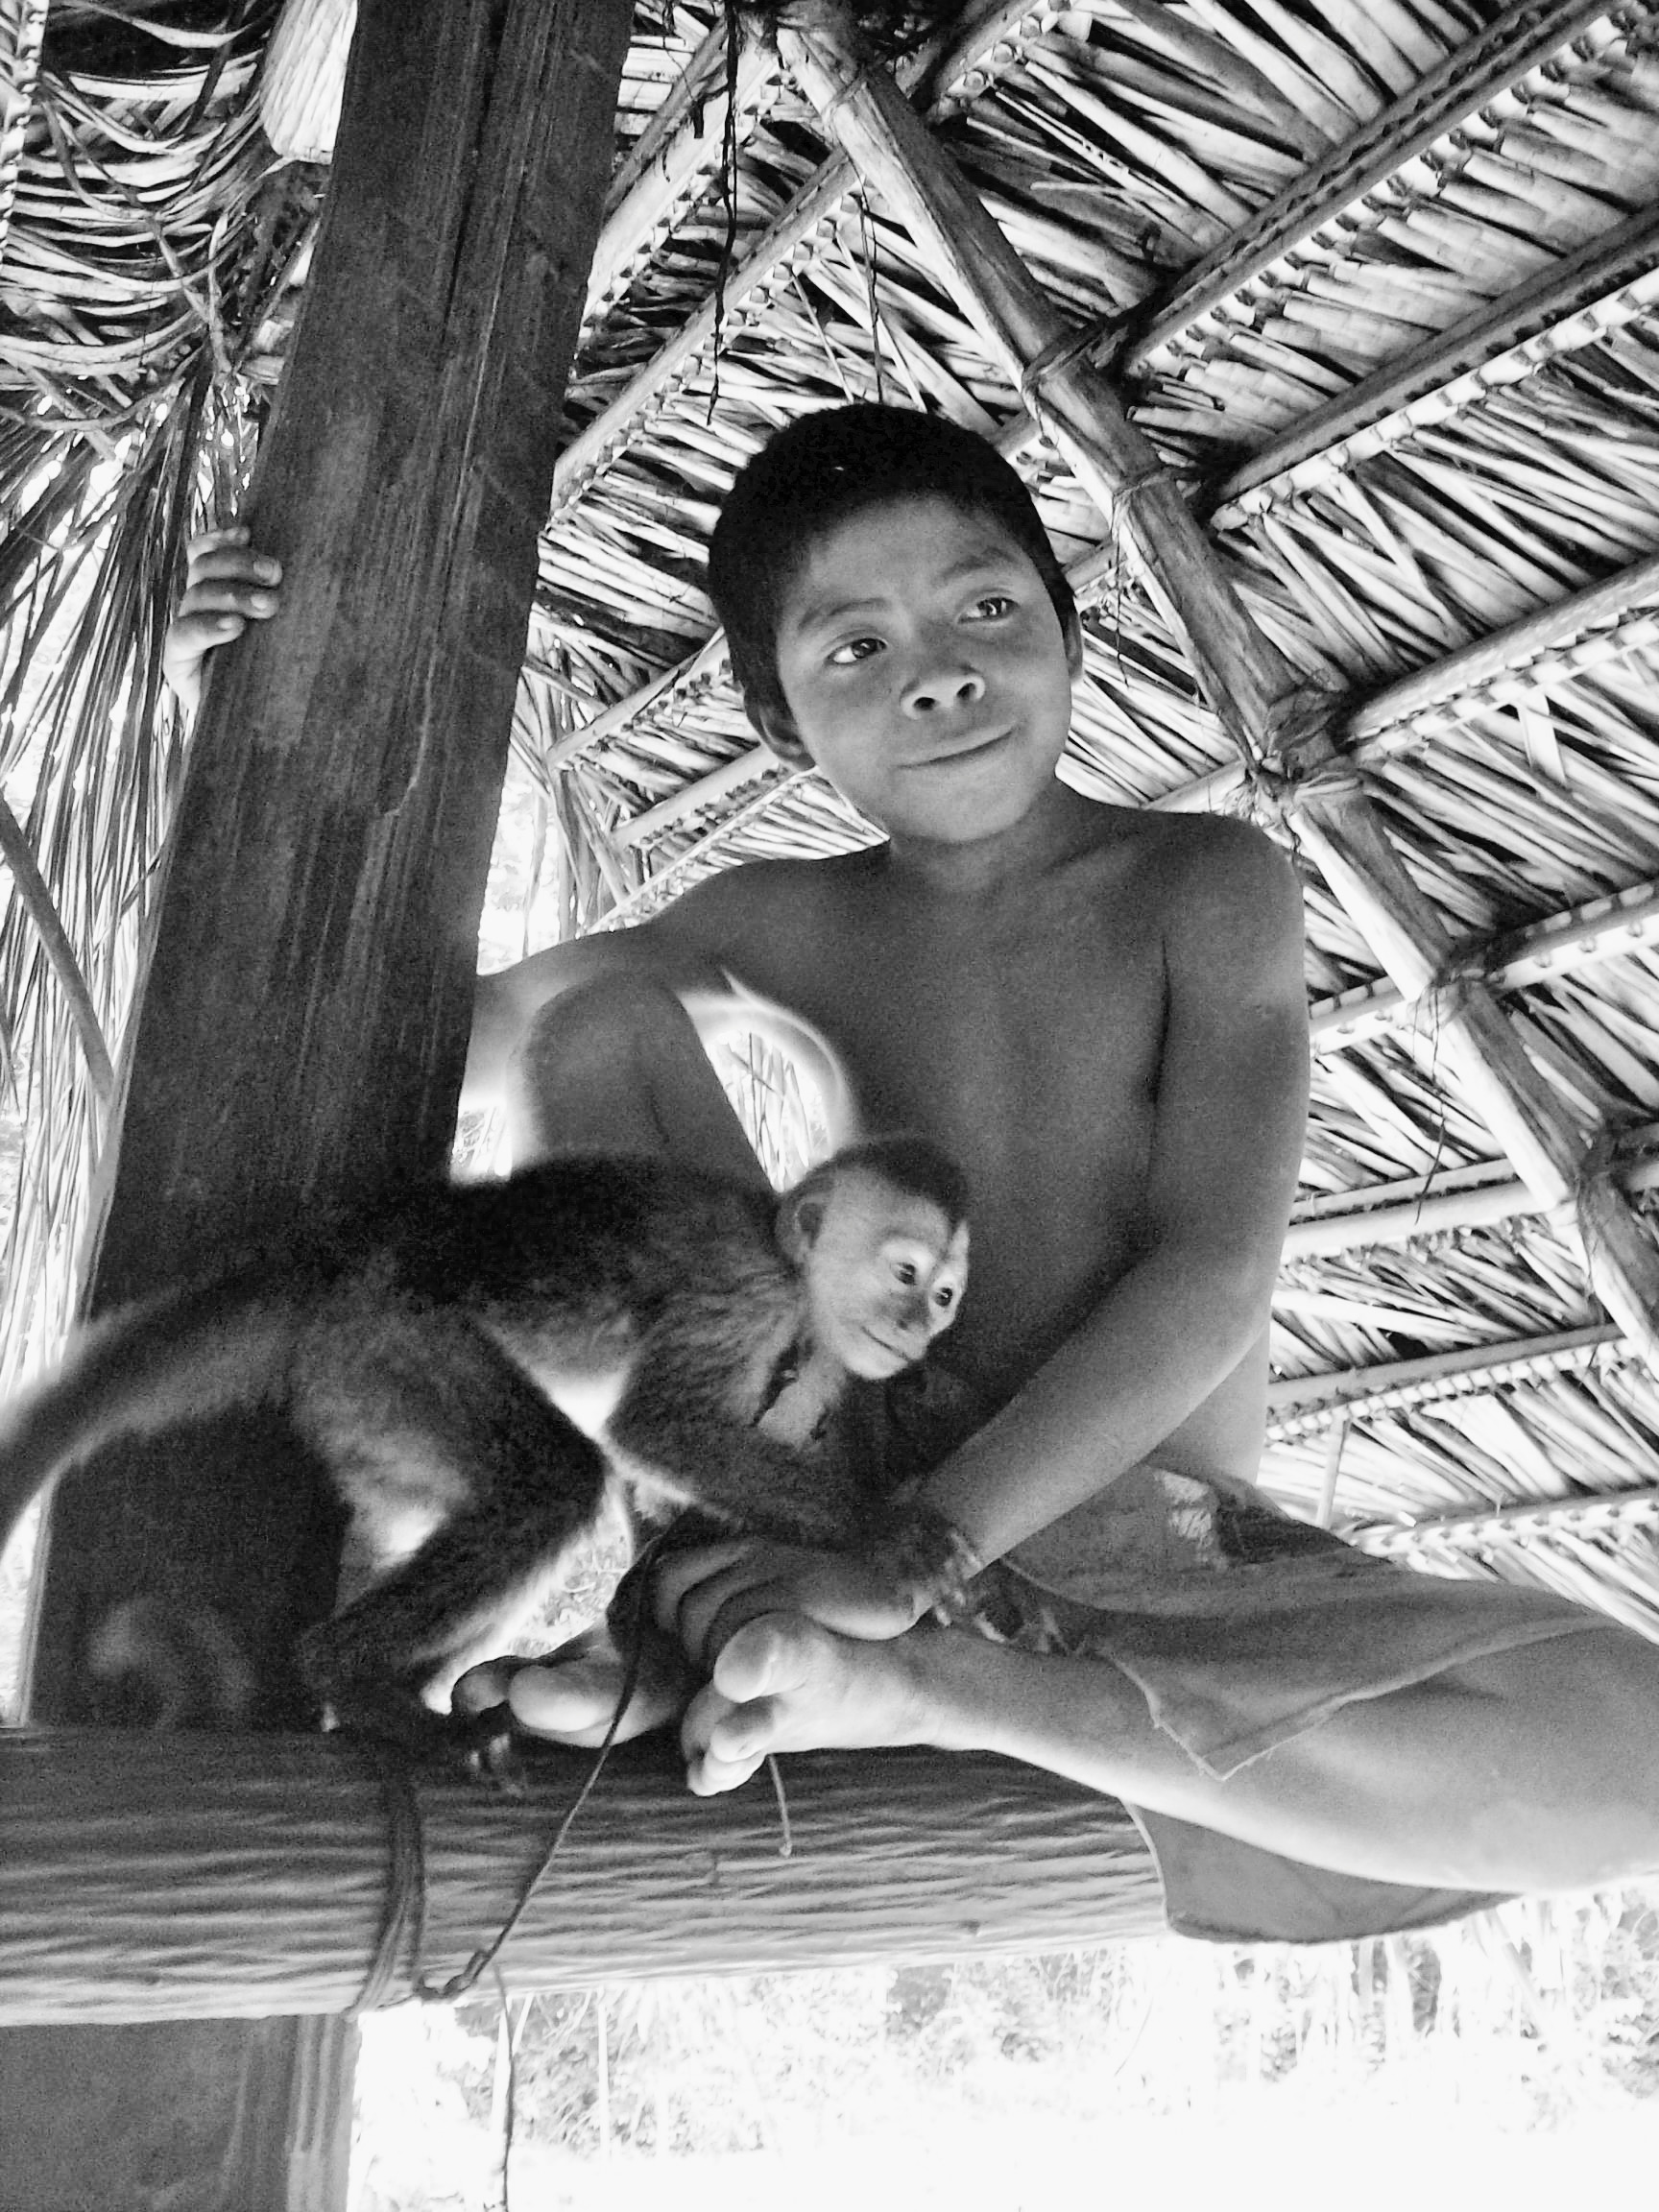
\includegraphics[width=97mm]{./imgs/100_4768}
%\caption{Takwari (ainda menino) sentado na viga do telhado de sua casa ao lado de um macaco cairara de criação (aldeia Juriti, 2007).}
%\end{figure}

\section{\emph{Awa mỹna}, a gente antiga}

Quando sozinho no mundo, o herói cultural \emph{Maira}\footnote{Quando
  utilizado na forma independente, o nome \emph{Mai(r)} ganha o sufixo
  nominal ``\emph{a}'' e sua consoante final r é recuperada, e aparece
  como \emph{Maira}. Se utilizado com outro substantivo, prevalece a
  forma original \emph{Mai}, como em \emph{Mai} \emph{nima,} ``animal de
      criação de Maíra''. Farei aqui uso das duas formas, a depender da
  situação.} fez a primeira mulher na Terra a partir de um tronco de
árvore (\emph{irakera,} ``aquilo que foi madeira''), e a criação de toda a
humanidade é atribuída a esse fato. A sequência inicial desse
acontecimento pode ser interpretada como uma variante do tema da Noiva
de Madeira (ou a Noiva Esculpida em Madeira), discutido por Lévi-Strauss
em \emph{Do Mel às Cinzas}, ``encontrado em regiões muito distantes do
continente, desde o Alasca, entre os Tlingit (\ldots{}) até a Bolívia, onde é
objeto de um mito tacana (\ldots{}) Entre os próprios Warrau, encontramos
este mito sob a forma da história de um rapaz solteiro que esculpe a
mulher num tronco de buriti'' (1967 {[}2004{]}, p. 201). Deste surgimento
da mulher esculpida na madeira pelo herói criador guajá e de sua
consequente gravidez, inicia"-se um ciclo com o nascimento de dois
meninos gêmeos, um chamado \emph{Maira} e o outro, ``Gambá''\footnote{Os
  nomes para o \emph{trickster} irmão de \emph{Maira}, Gambá
  (\emph{Didelphis marsupialis}, conhecido como ``mucura'' na Amazônia e
  sarigue em outras regiões do Brasil), podem ser \emph{Mukuxa'a}
  (``gambá'' com terminação final de nome próprio) ou mesmo \emph{Ajỹ},
  uma vez que o gambá é o principal avatar dos espectros \emph{Ajỹ}.
  Neste livro utilizo ``Gambá'' para me referir tanto ao irmão de
  \emph{Maira} quanto a mucura/sarigue em geral.} (Mucura ou Sarigue),
cujas aventuras deixam marcas visíveis na Terra até os dias atuais.
Combinando mitologia e sociologia, esse capítulo se interessa por um
tema clássico da etnologia sul"-americana --- e da antropologia --- definido
de maneira genérica como \emph{noção} \emph{de pessoa}. São discutidas
aqui as formas de \emph{subjetividade} \emph{awa}, a partir da descrição
dos componentes que marcam a humanidade (\emph{awatea} ``gente de
verdade''), as concepções sobre o corpo e a vitalidade, além de uma
antropologia interessada nas alegrias, tristezas, sonhos, onomástica,
comensalidade, enfim, elementos que compõem a própria existência.

À guisa de introdução, apresento uma sequência de acontecimentos míticos
cuja unidade das narrativas compõe um tema mais amplo, referente à
origem da primeira humanidade, pensados como \emph{awa mỹna}, a ``gente
de antigamente''.

Embora os Guajá narrem poucos mitos, penso que os transcritos adiante
são uma boa apresentação sobre os habitantes do mundo. Não é intenção
desta obra produzir análise mítica exaustiva; destaco"-os apenas por
serem ``histórias'' (\emph{mumu'ũ} --- ``ensinar/contar''; e
\emph{mumu'ũaena}, ``o que foi dito'', ``narrativa'') que os Guajá
relataram, muitas vezes para se referir a alguma situação ou explicar
determinadas coisas do mundo. Esses mitos aparecem transcritos com
repetições de frases e ideias, porém tais repetições são relativas à
forma como são contados (com pausas, anáforas e outros recursos que
marcam as narrativas). Assim, minha intenção é manter certo ritmo oral,
tal como alguns mitos parecem exigir. Ouvi essas narrações na aldeia
Juriti, Tiracambu e Awá e agradeço aos homens Wiraho, Takya, Pirama'ã,
Ka'awi'ia; na aldeia Tiracambu, Kamairu; e na aldeia Awá,
Hajkaramykỹa, Irakatakoa e Tatuxa'a. Também agradeço a Panapinuhũ (a
única mulher que o fez). Alguns foram relatados em português, e outros,
em Guajá.

\paragraph{A noiva de madeira}

\emph{Mairua} (``pai de Maira'', literalmente. \emph{Mai + t(r)ua} ``pai'')
não tinha esposa e passou muito tempo sozinho, até que um dia viu uma
árvore. A árvore tinha um tronco com formas que, ligeiramente, lembravam
um corpo humano. De seu tronco ramificavam galhos que, vagamente,
lembravam braços, e sua base se estendia pelo chão em raízes aéreas que
mais pareciam pernas. Após tanto procurar, o demiurgo escolheu essa
árvore para transformar em sua esposa. ``Eu não tenho esposa, vou fazer
deste pau a minha esposa'' disse \emph{Mairua}, que cortou um pedaço do
tronco e cantou, cantou, cantou; assim, fez aparecer as mãos, os braços,
seios, pés, pernas, cabeça, olhos, boca, nariz e vagina. E o tronco se
transformou em mulher. O herói também fez \emph{tapaja} --- a saia --- para
sua criação, e então ela se transformou em \emph{awa wahya}, mulher.
Quando essa primeira mulher surgiu, perguntou a \emph{Mairua}: ``Eu vi o
que você fez. Por que você me fez assim?'' ``É assim mesmo'', respondeu o
demiurgo, ``Eu não tinha esposa, e agora tenho''. Logo depois fizeram sexo
e ganharam filhos\footnote{Os mitos a seguir se relacionam diretamente
  com o ciclo mítico dos gêmeos Tupinambá trabalhados por Lévi"-Strauss
  em \emph{História de Lince} (ver Lévi"-Strauss, 1993).}.

\paragraph{A fuga de \emph{Mairua} (o pai de \emph{Maira})}

Houve uma época em que os pequizeiros só davam flores, e a fruta do
pequi (\emph{myky'á}) não existia. Assim, \emph{Mairua} falou para sua
esposa:

--- Vá pegar pequis para comermos!

Ela lhe responde que não e diz: --- dos pequizeiros só brotam florzinhas.

--- Então vá lá olhar!, disse \emph{Mairua}.

A ``mulher"-pau'' de \emph{Mairua} não quis ir e disse: --- Não vou, lá só
tem florzinhas e frutinhos bem pequenos, eu sei. Do pequizeiro não
nascem grandes frutos.

\emph{Mairua} ficou bravo com sua esposa.

--- Eu vou embora para longe de você. Você não é uma boa esposa para mim ---
disse o demiurgo.

\emph{Mairua} pegou suas flechas e foi embora. A esposa dele estava
grávida de gêmeos; um deles, muito sabido, por isso falou de dentro da
barriga para sua mãe:

--- \emph{Amỹ} (``mamãe''), vamos sair e procurar por meu pai!

Os meninos se chamavam \emph{Maira}\footnote{Tal como na mitologia
  Tupinambá, a mitologia Guajá narra as aventuras de \emph{Mairua}, que
  logo sairá de cena cedendo lugar a seu filho \emph{Maira} e seu irmão
  \emph{Gambá}, como veremos. Enquanto os Guajá destacam dois demiurgos,
  pai e filho respectivamente, na mitologia Tupinambá encontramos seis
  gerações do demiurgo: (1) Monam, o primeiro humano; (2) ``Maira"-Monam'';
  (3) seu filho ``Sumé'' que teve dois filhos; (4) ``Maira"-Pochy'', um dos
  netos de ``Maira"-Monam''; (5) o filho de ``Maira"-Pochy'', apenas chamado
  ``Maira''; (6) e ``Maira"-Ata, sexto e último demiurgo'' (Lévi"-Strauss,
  1993, p. 51 e 57). De acordo com Lévi"-Srauss: ``Ehrenreich, e Métraux em
      seguida, estima, provavelmente com razão, que as divindades que se
      sucedem e se substituem ao longo do relato constituem uma só; que são,
      como diz Métraux, desdobramentos umas das outras'' (Lévi"-Strauss, 1993,
  p. 56).} (tal como o pai) e \emph{Gambá}\footnote{Há uma versão desse
  mito que me foi narrada por meu amigo Hajkaramykỹa, que parece ser
  idêntica à de Thevet, trabalhada por Lévi"-Strauss em \emph{História de
  Lince}. De acordo com o relato de Hajkaramykỹa, a esposa de Maíra
  engravidou de \emph{Mairua} (pai de \emph{Maira}) e \emph{Mukuxa'a}
  (gambá) que seria o pai de Gambá, irmão de Maira. A mulher então seria
  mãe de gêmeos, porém com genitores diferentes. Na versão de Thevet
  para o mito Tupinambá, a mulher engravida de duas crianças a partir de
  pais diferentes: um dos gêmeos é filho de ``Maira"-Ata'', e o outro é
  fruto de um estupro cometido por ``Gambá'' (Lévi"-Strauss, 1993, p. 59).}
(\emph{Mukuxa'á}). A mulher, carregando os dois filhos no ventre, andou,
andou, andou, até encontrar as pegadas de \emph{Mairua}. Daí continuou
andando até encontrar folhas muito bonitas, e o bebê \emph{Maira} diz
para sua mãe:

--- \emph{Amỹ} (``mamãe''), pegue essas folhas para mim!

As folhas estavam repletas de marimbondos que picaram toda a mãe do
pequeno \emph{Maira}. Ela ficou muito machucada e brava por causa das
picadas que levou. Gritando, disse para o filho que carregava no ventre:

--- Por que você me pediu essas folhas? Eu estou toda machucada! Você quer
comer folhas? Por que você quer comer folhas? Agora, e por isso, eu vou
matar vocês dois.

A mulher começou a bater na própria barriga com muita força, ``pá, pá,
pá'', certa de matar os gêmeos. Surpreendentemente, apesar das diversas
pancadas, \emph{Maira} e \emph{Gambá} não morrem. Eles são muito fortes.
Depois das pancadas que a mãe desferiu na própria barriga, \emph{Maira}
cessa o diálogo com sua mãe.

Então, a mãe lhe pergunta:

--- Onde está o seu pai, que eu não o acho?

\emph{Maira}, de dentro da barriga, nada responde, pois está zangado com
sua mãe. A mulher continuou a caminhar pela floresta em busca de seu
marido, até que encontrou o rastro de alguém. Ela não sabia que se
tratava de pegadas de onças e imaginou ser o caminho aberto por seu
marido, \emph{Mairua}. E pensou:

--- Acho que meu marido está por aqui. Sim, ele foi por aqui mesmo.

E seguiu pela trilha.

\paragraph{A aldeia das onças}

A esposa de \emph{Mairua} seguiu pela trilha até encontrar uma mulher,
jovem e bela. Era uma ``mulher"-onça'' (\emph{jawa wahya}), esposa de um
homem"-onça (\emph{jawara}). Essa mulher estava cozinhando animais da
floresta como caititus e veados. Nessa época, as onças, que eram humanos
--- embora um pouco diferentes, pois também gostavam de carne crua ---,
dominavam o fogo. De dia eram gente e à noite viravam onça e saíam para
caçar. A mulher"-onça enxergou a esposa de \emph{Mairua} e a chamou:

--- Venha para cá! --- disse a onça.

--- Estou procurando meu marido, você o viu? Ele me largou --- disse a
esposa de \emph{Mairua}.

--- Não eu não o vi. A minha casa é aqui e eu não vi ninguém passar. Eu
sou uma onça, o meu marido também é uma onça, nós não somos \emph{awa}.
Fique aqui conosco, você será a minha neta (\emph{hamijarua}). Eu vou
criar você como uma neta --- falou"-lhe a mulher"-onça.

A mulher de \emph{Mairua} aceitou a proposta. Assim a mulher"-onça
retirou algumas palhas e prontamente construiu uma casa em forma de
tocaia, bem fechada, para que a mulher lá se instalasse sem que seu
marido"-onça (um devorador de carne humana) a visse.

--- A partir de agora você vai dormir nesta casa, disse a mulher"-onça. O
seu marido (\emph{Mairua}) foi para muito longe, e você não vai mais
encontrá"-lo.

No final da tarde, o marido da onça voltou de uma caçada. Por isso sua
esposa"-onça falou baixinho:

--- (sussurando) O meu marido está chegando, eu consigo ouvi"-lo, shhhhhh!

O marido"-onça traz consigo alguns pedaços de carne e cabeças de caititu
e veado. Os outros pedaços ele comeu crus, ainda na floresta. No caminho
para sua casa ele encontrou as pegadas da esposa de \emph{Mairua} e, ao
chegar em casa, jogou a carne no chão perguntando para a esposa:

--- Você viu algum humano (\emph{awa}) por aqui? Eu encontrei pegadas aqui
perto.

--- Não, eu não vi nenhum humano, estou sozinha em casa --- respondeu a
mulher"-onça.

--- Mas eu encontrei as pegadas de um humano no caminho, e as pegadas
vinham nesta direção --- insistiu o homem.

--- Não há ninguém aqui. Eu vi uma mulher, mas ela foi"-se embora por ali
(apontando para uma trilha) --- disse a mulher"-onça.

--- Não, ela não foi embora! --- disse o marido"-onça, convencido de que a
humana ainda estava em sua aldeia.

De repente um vento soprou, e a onça consegui sentir o cheiro da mulher
que vinha de dentro da sua casa"-tocaia, pois de todos os animais a onça
é o que melhor sente o cheiro dos humanos. Quando o marido"-onça viu a
tocaia, concluiu:

--- Ah, aqui está! Essa tocaia não estava aqui antes, alguém a construiu.

O homem"-onça invadiu o abrigo, mas sua esposa gritou em cima:

--- Não coma ela! Ela é nossa \emph{harapihianã} (parente por afinidade).
Você já comeu muito caititu, veado e outros bichos no mato, para que
comer essa humana?

Mas a onça, ``crau'', comeu"-lhe a cabeça. Depois comeu tudo: os braços, a
pele, comeu tudo. Tirou a tripa, tirou tudo e comeu; não tem mais a mãe
de \emph{Maira}. Só sobraram"-lhe os filhos na barriga, que a esposa"-onça
pediu para comer:

--- Você está comendo toda essa mulher, então me dê os filhos dela para
que eu também os devore. Deixe eu comer também!

--- Está bem --- disse o marido.

\paragraph{O nascimento dos gêmeos}

Com o auxílio de uma faca, o homem"-onça abriu a barriga da mulher morta,
tirou as duas crianças, e deu à sua esposa para que comesse. Ela,
bastante chateada, passou a maldizer o marido por ter feito tamanha
maldade àquela mulher. Mesmo assim, para agradar o marido, a mulher"-onça
colocou os dois bebês perto de pedaços de animais que seriam limpos por
ela antes de assados\footnote{Em outra versão, a mulher"-onça tem piedade
  das crianças e quem decide cozinhar os gêmeos é outra mulher (também
  onça) da mesma aldeia.}. Após limpar os animais caçados, ela pegou os
dois bebês \emph{Maira} e \emph{Gambá} e pensou:

--- Vou cozinhá"-los mesmo!

Pôs água dentro de uma panela e em seguida colocou os gêmeos, mas eles
pularam para fora da panela.

--- Que diabos é isso? --- pensou a mulher.

Colocou"-os novamente dentro da panela, e novamente eles pularam para
fora. Assim aconteceu seguidas vezes. Eles eram muito espertos. Ela os
botava para dentro da panela e eles pulavam para fora ao sentir a água
quente. A mulher"-onça então disse:

--- \emph{Ariku ta hanima neme}, ``vou criá"-los como (ficar com eles
como/transformá"-los em) meus seres de criação''. Eles são meus
\emph{harapihianã} (afins), eu vou criá"-los como se fossem meus netos.
Vou pô"-los no rio.

Por isso, aproveitou que seu marido fora caçar na floresta e colocou os
dois meninos, que ainda estavam na placenta, dentro do rio para acabar
de gestarem. O marido"-onça, embora possuísse arco e flecha, caçava
somente com suas garras e dentes. Passado algum tempo, os gêmeos
cresceram, cresceram e cresceram, a placenta rasgou e os dois meninos
nasceram. Assim que saíram da placenta procuraram pela mãe:

--- Cadê a nossa mãe? Onde está nossa mãe? --- procuravam os gêmeos.

A mulher onça respondeu:

--- A mãe de vocês foi embora. Agora eu sou a mãe de vocês. Podem
acreditar em mim, eu sou a mãe mesmo. Eu mesmo!

--- E cadê o nosso pai? --- perguntaram

--- O pai de vocês foi caçar. Foi caçar caititu, veados, queixadas ---
referindo"-se ao marido"-onça. Comam essa carne aqui --- ofereceu a mulher
aos meninos.

A mulher"-onça deu para eles comerem um pouco de uma carne bem macia,
pois eles já tinham dentes, e \emph{Gambá} comeu um pouco da carne.
Passado um tempo, o homem"-onça voltou de sua caçada trazendo caititus,
veados e queixadas. Quando viu os meninos, perguntou:

--- Quem são essas duas crianças?

--- São nossos netos --- disse a mulher"-onça. --- Eles apareceram aqui,
deixe eles aqui, não os coma! Eu vou criá"-los --- disse ela ao
marido.

--- Pode deixar, eu não vou comê"-los --- respondeu a onça.

Então eles cresceram, cresceram, cresceram. Fizeram suas próprias
flechinhas. E nessa época mataram muitos passarinhos. E chegaram em casa
falando:

--- Vovozinha, nós matamos passarinhos!

--- Quantos passarinhos vocês mataram?, perguntou a avó.

--- Estão aqui, olha quantos, vovozinha. Matamos dezenas de passarinhos,
vovozinha. Matamos tantos que parecem capelães, de tanto que matamos.
Caçamos chora"-chuva preto, juriti"-gemedeira, urus, nhambus, pariris,
rolinhas, pombos, tá tudo aqui, vovozinha!

A onça"-avó ficou feliz com a caçada de seus netinhos e se deliciou com
tantos pássaros. Ela cozinhou tudo em panelas, do jeito que a gente"-onça
gostava de comer. \emph{Maira} estava se tornando um grande caçador já em sua
primeira infância. Eles continuaram crescendo, crescendo, crescendo\ldots{}
Passado algum tempo, os gêmeos tornaram"-se adultos.

\asterisc

A partir de agora, \emph{Maira} e \emph{Ajỹ} inauguram um ciclo de
acontecimentos que dão origem a muitas das coisas do mundo, tal como os
Guajá conhecem hoje; além de explicar, em parte, o aparecimento dos
humanos. Vejamos o que nos interessa, por hora.

\paragraph{O surgimento dos inajás e das ariranhas}

\emph{Maira} pensou e disse para seu irmão, \emph{Gambá}:

--- Vamos fazer o inajá aqui.

--- Para quê? --- perguntou \emph{Gambá}

--- Para comer --- respondeu \emph{Maira}

\emph{Maira} e \emph{Gambá}, juntos, fizeram brotar cachos de inajá
instantaneamente. Os inajás feitos por \emph{Maira} eram os amarelos
dourados (\emph{pirỹma'a} ``avermelhado''), enquanto \emph{Gambá} fez
inajás brancos, que são muito ruins. Havia muitos inajás, e eles
resolveram levar para sua mãe"-onça. Fizeram dois \emph{marakũa}
(sacolas/mochilas confeccionadas com folhas frescas). \emph{Maira} levou
um \emph{marakũa}, e \emph{Gambá} levou o outro. A mulher"-onça estava em
casa, porém não conhecia inajás. Quando ela viu os gêmeos voltando,
falou:

--- Venham logo! Onde vocês estavam? O meu marido"-onça vai comê"-los se
ficarem sozinhos pela floresta.

Quando chegaram em casa, falaram:

--- Mãe, trouxemos inajás.

--- Vocês sabem produzir o inajá?

--- Sim, nós sabemos e fizemos, aqui está! --- disse \emph{Maira}.

A mãe"-onça colocou os inajás no fogo e os cozinhou. Depois de cozidos,
comeu e disse:

--- Nossa, mas esses inajás são bem grandes e muito gostosos\footnote{Vale
  lembrar que, no tempo dos mitos, os frutos eram maiores do que são nos
  tempos atuais.}. Onde vocês conseguiram? Eu quero ver esse inajazeiro,
vocês me levam até lá?

--- Vamos lá, é por aqui! --- disseram os gêmeos convidando a mãe para
coletar mais inajás\emph{.}

A mãe"-onça foi seguindo seus netos (ou ``filhos'') até chegar ao
inajazeiro. Era uma árvore magnífica que produzia inajás muito grandes,
maiores do que os encontrados atualmente. Ela coletou muito desses
frutos e voltou para casa com seus filhos para cozinhá"-los. Chegando à
aldeia, cozinhou"-os e enquanto comia jogava suas cascas perto de casa. O
\emph{Jaku Jara} (um jacu humano), que era muito sabido, então falou
para \emph{Maira}:

--- Meu \emph{harapihianã} (``afim''), você mora junto com a onça, mas você
não deve morar junto dela. Ela não é sua mãe como você pensa. Ela comeu
a sua mãe de verdade. Ela te pegou para criar e se tornou sua avó, mas
ela nunca foi sua mãe.

--- É mesmo? --- disse \emph{Maira}, atônito. --- Então espere, pois eu vou
fazê"-las (as onças) virarem ariranhas (\emph{jawatara}).

Nisso, o homem"-onça volta de sua caçada habitual trazendo porcos,
caititus, veados mateiros e veados fobocas. A onça não caçava antas,
pois este animal tem o couro muito duro. Quando a onça viu os inajás,
perguntou:

--- O que é isso? Quem fez esses frutos?

--- Os nossos netos sabem fazer inajá; foram eles que fizeram --- disse a
esposa"-onça. --- Eles fizeram muitos inajazeiros por aí, muitos, muitos.

--- Então vamos comer! --- disse o marido"-onça.

--- Vá lá, eu vou ficar aqui --- respondeu"-lhe a esposa.

O homem"-onça comeu muitos inajás, junto com as outras onças; e pegaram
outros para levar para casa. Na volta, enquanto a esposa"-onça estava
limpando os animais em casa para cozinhar, as onças que voltavam
passaram por uma ponte no caminho. Enquanto passavam pela ponte,
\emph{Maira} conseguiu derrubá"-la dentro d'água, fazendo com que as
onças caíssem. Ao cair, elas foram devoradas por piranhas
(\emph{ipinẽa}) muito grandes, e seus ossos viraram ariranhas. As
ariranhas, que eram os ossos das onças, foram embora nas águas. Logo
depois, outro grupo de onças voltava pela mesma ponte, e \emph{Maira}
conseguiu derrubar a ponte novamente, fazendo com que esse grupo de
onças também caísse n'água. As piranhas também as devoraram, e seus
ossos também viraram ariranhas.

Em seguida, mais onças vieram pelo caminho, e \emph{Maira}, junto com
seu irmão, \emph{Gambá,} conseguiu transformar as onças em veados,
fazendo com que os veados saíssem correndo pela mata. \emph{Maira} fez
isso várias vezes. Certa hora, o demiurgo sentiu vontade de defecar e
pediu para que seu irmão continuasse transformando as onças em
veados"-mateiros (\emph{arapaha}) e veados"-fobocas (\emph{arapaha'í}),
mas o alertou:

--- Eu vou cagar. Não faça nada de errado e continue o que estamos
fazendo!

Enquanto \emph{Maira} fazia suas necessidades, ficou observando o irmão.
Uma onça veio pela ponte e \emph{Gambá}, meio atrapalhado, não conseguiu
transformá"-la em veado, deixando"-a na forma de onça. \emph{Maira} voltou
rapidamente e esbravejou com \emph{Gambá}:

--- Você não está fazendo direito. Não faça desse jeito ruim, você deve
transformá"-las em veados.

---Tá bom --- respondeu \emph{Gambá}.

\emph{Maira} voltou para suas necessidades, e novamente \emph{Gambá}
deixou as onças passarem sem que fossem transformadas em veados. E
\emph{Maira} brigou novamente com seu irmão:

--- Você não fez direito! Deixou as onças irem embora, agora elas
vão nos comer para sempre. Vamos voltar para casa!

Quando retornaram para casa, a mãe"-onça lhes perguntou:

--- Onde está meu marido?

--- Não sei. Parece que ele está comendo inajás. Depois virá para casa ---
responderam os dois de maneira dissimulada.

\paragraph{O surgimento do gavião}

A mãe"-onça de \emph{Maira} pede que seu filho cate piolhos (\emph{ikya})
de sua cabeça. Enquanto ele o fazia, a mãe"-onça adormeceu.
Aproveitando"-se da situação e para vingar sua verdadeira mãe que fora
morta pelas onças, \emph{Maira} e \emph{Gambá} cortaram"-lhe a cabeça.
Depois pegaram a cabeça da onça, fizeram"-lhe nascer penas e ela se
transformou em gavião. A mãe"-onça ficou deitada sem cabeça em sua rede,
e \emph{Maira} foi embora procurar seu pai, \emph{Mairua}.

\paragraph{Coda}

A partir desse episódio, quando \emph{Maira} e \emph{Gambá} matam a
mãe"-onça e vão embora pelo mundo, um conjunto de mitos consolida os
gêmeos como precursores da humanidade, de quem todos os Guajá
descenderiam. É \emph{Maira} que traz a especiação dos seres e, após a
Terra (\emph{wya}) estar pronta, com sua paisagem atual concretizada,
outros humanos selvagens (\emph{mihua}) atentam contra a vida de
\emph{Maira} envenenando"-o. E ele, mesmo sobrevivendo, parte para o céu
junto com seu irmão gêmeo, e lá vivem até hoje.

\section{\emph{Awatea}, gente de verdade}

Utilizado por diversos grupos Tupi"-Guarani da Amazônia --- como os
Parakanã (Fausto, 2001), Asuriní do Xingu (Müller, 1993), Aikewara
(Calheiros, 2014, p. 7), Ka'apor (Balée, 1994) ---, o termo \emph{awa}
aparece aqui como a forma pela qual esse povo se identifica, encontrando
em ``humano'' ou ``gente'' as melhores traduções, em oposição a outros
termos como \emph{kamara} (outros indígenas), \emph{karaia} (não
indígena) e \emph{mihua} (gente selvagem), como veremos. \emph{Awa} são
homens e mulheres, \emph{wanihã} (♂) e \emph{wahya} (♀) de um
mesmo universo. Os Guajá se pensam como \emph{awatea} (``humano'' +
\emph{-te} ``real, verdadeiro''), idêntico inclusive ao termo na língua
Parakanã (Fausto, 2001, p. 39) que pode ser traduzido como ``gente de
verdade'' (ver também Cormier, 2003, p. 89). Muito mais do que ``a
humanidade como espécie natural'', a categoria \emph{awa} denota uma
``condição social da pessoa'' (Viveiros de Castro, 2002, p. 371), que
neste caso (bem como em tantos outros povos ameríndios) consiste em uma
composição própria do corpo, além de um gradiente social formado por uma
série de oposições que se inicia nos humanos próximos e se estende às
esferas de parentes mais distantes, até chegar aos grupos inimigos e
outros seres perigosos como os seres"-espectro \emph{Ajỹ}.

Fisiologicamente, os Guajá definem a pessoa humana como constituída por
três elementos característicos: \emph{ipirera}, \emph{hajtekera} e
\emph{ha'aera}, respectivamente. Ou, como traduzem para o português:
``meu couro'' (\emph{hapirera}), ``carne'' (\emph{hajtekera}) e ``raiva''
(\emph{ha'aera}). Em linhas gerais, e como gostam de ilustrar, quando
uma pessoa morre, seu ``couro'' permanece na Terra até apodrecer, e sua
``carne'' vai para o \emph{iwa} (um conjunto de patamares celestes);
enquanto a ``raiva'' segue para a floresta (\emph{ka'a}), para o
mato, de preferência para os locais recônditos, e se transforma em \emph{ajỹ}
(espectros necrófagos que vivem na floresta, atacam os humanos com
doenças e têm os gambás como animais de criação). Noções centrais para o
entendimento da sociocosmologia \emph{awa}, \emph{ipirera},
\emph{hajtekera} e \emph{ha'aera} são os princípios que promovem a vida
e possibilitam a separação da pessoa após a morte. Poderíamos traduzir
grosseiramente \emph{ipirera} por ``corpo"-pele''; \emph{hajtekera} por
``vitalidade'' (cujo correspondente ocidental, apenas como paralelo, seria
``alma''); e o \emph{ha'aera}, por ``raiva'' ou ``alma penada''. Tentarei
esboçar aqui como tais ideias tornam complexo o dualismo corpo e alma/ou
material e espiritual, e não são representações do que seria a pessoa
humana em seus aspectos material e imaterial. Pelo contrário, esses três
elementos embaralham de alguma forma noções fisiológicas centrais --- como
anatomia e sintomatologia ---, pois aqui, elementos do corpo físico
transcendem a ideia de ``físico''. Em outras palavras e de maneira bem
direta, o corpo aqui é muito mais (ou menos) do que o suporte do
\emph{hajtekera} --- alguns elementos do corpo também são o próprio
\emph{hajtekera}, e isso nos fornece uma terminologia apropriada para o
entendimento das relações humanas.

\section{Viver, morrer}

Antes do contato, quando a morte de alguém ocorria o mais comum era
abandonar a área onde viviam, deixando para trás o cadáver
(\emph{ipirera}). Durante as caminhadas, qualquer espaço servia para
deixar um corpo: no meio do mato longe do caminho (\emph{pea}), em um
buraco dentre tantos feitos pela erosão ou animais na floresta e mesmo
dentro de uma árvore oca e caída, apodrecida na paisagem. O morto era
deixado para trás. Se a morte ocorresse dentro de casa, deixavam o
cadáver em sua rede e derrubavam a casa (\emph{tapãja} ``tapiri'') sobre
o morto, partindo para longe, e montavam uma nova aldeia (que, como
vimos, muitas vezes consistia em uma única casa). Se a morte ocorresse
durante uma caminhada, simplesmente abandonavam o corpo e permaneciam
longe da área de morte por um longo período de tempo. A única exceção
são os recém"-nascidos, os natimortos. Quando ocorre de um bebê morrer no
parto, e só nesses casos, ele é enterrado dentro de casa, pois as
pessoas ainda não se ``acostumaram'' (\emph{amimakwa}) à criança. As
pessoas evitam locais onde ocorreram mortes recentes ou com sepulturas,
uma vez que os fantasmas \emph{ajỹ} costumam frequentar tais locais.
Desde o contato com a \textsc{funai}, foram criadas próximas às aldeias áreas
para ``enterro'', é prática dos funcionários do posto enterrar as pessoas
mortas. Quem faz esse trabalho desagradável são os \emph{karaia} da
\textsc{funai}, já que os Guajá pouco manuseiam ou enterram seus mortos em
sepulturas. Desde a fixação em aldeias a partir do contato, muitas
pessoas faleceram de gripe e malária, e os Guajá passaram a conviver com
o ``mal"-estar'' de viver próximos aos mortos. No ``tempo do mato''
(\emph{imỹna} ``antigamente''), os velhos e moribundos eram abandonados,
pois quando a morte se aproximava não era seguro permanecer ao lado de
alguém prestes a sucumbir. Até os dias de hoje, as pessoas muito velhas
podem (ou não) receber um tratamento de abandono. Uma das situações que
mais chamavam atenção dos funcionários da frente de atração na época do
contato (disse"-me certa vez um funcionário aposentado que conheci) era o
fato de muitas pessoas aparecerem para o contato afirmando terem deixado
para trás seus parentes mais velhos (pais e avós), uma vez que esses se
recusavam a se encontrar com os \emph{karaia}. Os Guajá que passaram a
viver nas imediações do \textsc{pin}, por outro lado, nunca mais voltariam a
viver com esses velhos que foram deixados para trás para morrer.
Kamairua, um amigo da aldeia Tiracambu, se lembra do pai --- nos anos de
fuga para evitar o contato --- que pedia para ficar para trás e exortava os
parentes a fugirem para longe, dizendo que estava velho, sem forças para
fugir e que iria morrer sozinho.

Como exemplo, \emph{Amirixa'a} é mãe de Muturuhũ, um homem importante na
aldeia Juriti. Ela é a mulher mais velha dessa aldeia, com idade
estimada em 89 anos (em 2008). Dentre todos, ela é a única que vive em
um tapiri, na periferia da aldeia; e dentre as mulheres, só ela veste
uma saia trançada com fibra de tucum, como era comum entre os
Guajá\footnote{Hoje as mulheres preferem saias tecidas com linha e panos
  que ganham ou retiram de outras peças de roupas.}. Amirixa'a produz a
própria comida: carrega pesadas cargas com macaxeira ou banana que
retira da roça; caça tatus e jabotis por conta própria. Ninguém a ajuda,
em nada. Se ela não procurar comida, não comerá. Devido a sua idade
avançada, sua dieta é livre de restrições, come qualquer coisa,
inclusive alimentos que causariam mal a outras mulheres: desde vísceras
variadas e fetos de inúmeros animais a carne de veados mateiros
(\emph{arapaha)} e foboca (\emph{arapaha'i}). Há também uma dieta de
``antigamente'' (\emph{imỹna}), composta por animais considerados
``repugnantes'' (\emph{manyhỹ}) aos olhos dos jovens, mas que os velhos
podem e até gostam de comer, como uma rã chamada \emph{iwea}, feita
assada na brasa, e diversas espécies de ratos (\emph{awijỹa}) que depois
de limpos são assados em espetinhos. Antes do contato comiam isso tudo,
algo como uma ``dieta do mato'' (\emph{ka'a nimi'ũa} ``comida da
floresta''), porém hoje em dia é comida de gente velha, pois essas
pessoas não passam mal com alimento quase nenhum.

Embora Amirixa'a receba esporadicamente pedaços de carne do grupo do seu
filho, ela possui seu próprio fogo e come separadamente das outras
pessoas. Pira'ima'ã, um de seus netos, explicou"-me que Amirixa'a está
velha (\emph{tamỹ}) e não adianta o quanto de comida que deem a ela,
pois não vai se fortalecer. Não consegue se relacionar, pois se ela está
\emph{velha} está \emph{surda}, e se está \emph{surda} vai
\emph{morrer}. A surdez é o sinal mais evidente da presença (ou chegada)
da morte. E se tornar velho e surdo (necessariamente nesta ordem) é o
destino a que todos os Guajá estão sujeitos. \emph{Japijakoa myty}
(``ouvido entupido'') é uma das imagens mais utilizadas para se referirem
à velhice. Uma pessoa muito velha é uma pessoa surda; e uma pessoa surda
é um quase"-morto.

Os velhos não conversam nem se relacionam porque não ouvem, a velhice
extrema como a de Amirixa'a é uma situação de não"-relação, porque ela
está muito velha para se casar novamente, conversar, cantar, ou qualquer
outra coisa. O fato de que, por consequência da velhice, as pessoas
dispensem menos cuidados a Amirixa'a não representa um descuido
deliberado, mas a aceitação de que o período de vida dela chegou ao fim
e que seu ``princípio vital'' (\emph{hajtekera}), responsável justamente
pela sua ``vitalidade'' (uma outra tradução para \emph{hajtekera}), não
mais lhe habita. A surdez, ela mesma, é associada à ausência do
\emph{haitekera}. Como Wiraho pontuou"-me certa vez: ``nós estamos tão
acostumados com Amirixa'a, de vê"-la todo dia, que quando ela morrer
vamos pensar --- Ah, ela não está mais conosco!, e vamos ficar muito
tristes''\footnote{A ideia de abandono, e até mesmo aniquilamento dos
  idosos, é comum a diversos povos ameríndios. Descola apresenta a
  situação de uma velha que estava morrendo de doença em uma das casas
  que vivia e as pessoas tristemente diziam a ela: ``você está morta
      vovozinha, está morta'', enquanto ela ainda falava e pedia o que comer.
  E, diferente de outras doenças, as pessoas não procuravam intervir com
  medicamentos e outros tipos de ajuda. A mulher velha já era um cadáver
  (Descola, 2006, pp. 407 e 409).}. Nas noites de cantoria, quando seu filho
adentrava a \emph{takaja} para ir ao \emph{iwa}, a velha cantava
baixinho, de dentro de sua pequenina casa, para auxiliar o filho durante
sua viagem celeste. Em tais momentos todos paravam para ouvi"-la,
alertando uns aos outros: ``\emph{Kwy!}\footnote{O ``\emph{kwy}'' é uma
  interjeição utilizada para exprimir surpresa, que pode ser comparado a
  ``Nossa Senhora!'', como falado em boa parte do Brasil.},
\emph{Amirixa'a jã}'' (``Olhem, Amirixa'á está cantando!''); a mulher
parecia querer lembrar a todos que, mesmo solitária, ainda estava viva.

A convivência de pessoas em velhice extrema com outras em idades menos
avançadas é um ``fenômeno'' que passou a ocorrer com mais frequência após
o contato com a \textsc{funai}. Desde a radical mudança na aparência e
funcionamento das aldeias, os velhos definham nas aldeias até morrer; e
quando morrem, os funcionários dos \textsc{pin} se encarregam de enterrá"-los em
local próximo e reservado como cemitério. Nesse meio tempo, os Guajá ---
praticamente todos eles --- abandonam a aldeia por muitos dias e se
refugiam na floresta; pois, tal como sabemos a partir de outros povos
Tupi, os Guajá também têm pavor de cadáveres. Mais adiante veremos
melhor esse ponto. O luto, portanto, é um processo de esquecimento
(\emph{imahare}) dos nomes, eventos e lugares relacionados à pessoa
morta que, aos poucos, é apagada da memória. Juriximatỹa certa vez me
contou ter ficado muito triste com a morte de seu cunhado To'oa; por
isso foi para a floresta logo que soube do fato e lá permaneceu durante
muitos dias, a fim de esquecer o falecido.

Da mesma maneira, por parte do morto, a morte é, da mesma forma,
``esquecer'' que foi vivo. Essa teoria é muito atuante entre os Guajá, que
dizem que ao chegarem no céu, após morrerem, se lembram pouco da vida na
Terra; e, à medida que se aproximam dos \emph{karawara}, vão perdendo a
memória, até o completo esquecimento de que foram vivos. Esse argumento,
a despeito de sua elegante simplicidade, é talvez o argumento mais
importante sobre o que seja ``morrer'' (\emph{manũ}) para os Guajá. Não é
possível explicar a subida definitiva do \emph{hajtekera} para o
\emph{iwa} (em outras palavras, \emph{morrer}) sem mencionar o
esquecimento natural da vida terrena que o \emph{hajtekera}
experimentará no céu (\emph{iwa}). Por isso, discordo da interpretação
de Cormier --- baseada em outros autores (Geertz, por exemplo) --- ao
sustentar que a falta de compreensão genealógica dos Guajá pode ser
considerada ``amnésia genealógica'' (Cormier, 2003, pp. 74--76). Os Guajá
simplesmente não querem falar dos mortos, e o ``esquecimento''
(\emph{imahare} --- ``esquecer'' ou ``não saber'') é um aspecto constituinte
do processo de luto e da morte. Eles esquecem o nome de pessoas das
gerações acima não porque sejam incapazes de lembrar, mas, ao contrário,
porque lutam para esquecer. Esse é um ``problema'' dos Guajá e de boa
parte da Amazônia indígena (ver Taylor, 1993).

Quando do falecimento de uma pessoa (\emph{manũ} --- ``morrer''), diz"-se
\emph{hajtekera} \emph{oho iwape} (``\emph{hajtekera} foi para o
\emph{iwa}''). E, depois de falecida, diz"-se \emph{hajtekera} \emph{ikwẽ
iwape} (``a pessoa, ou \emph{hajtekera}, permanece no \emph{iwa}''). A
mim, ao falarem sobre a morte, era comum mencionarem em português que
determinada pessoa ``morreu'' ou ``subiu'', tal como se fossem sinônimos
para as situações de morte\footnote{É bom lembrar que, assim como no
  português, os verbos ``subir'' e ``morrer'' são diferentes na língua
  Guajá. \emph{Ipii} seria o equivalente a ``subir'' em português,
  utilizado, por exemplo, ao se referir a alguém que tenha subido em uma
  árvore: \emph{ipi ira rehe} --- ``ele subiu na árvore''. Além desses,
  pode"-se dizer que algum indivíduo morreu utilizando"-se a expressão
  \emph{oho iwape}, nesse caso, ``foi para o céu''.}. Ao traduzir para o
português a ``morte'' por ``subida'', demonstram que o essencial da ideia de
morte (\emph{manũ}) é o deslocamento espacial da substância
\emph{hajtekera} --- que traduzo por ``princípio vital'' --- da Terra para o
céu. Porém, em diversas situações em que o \emph{hajtekera} abandona o
corpo, não obrigatoriamente implica morte. Nos dias de verão, quando
preparam a \emph{takaja} e homens de diferentes idades cantam com os
\emph{karawara} e com os mortos (o que discutiremos no último capítulo),
encontramos um desses casos. Também, se uma pessoa se expõe a perigos e
privações, a reação natural é perder o seu \emph{hajtekera}. Vejamos
três situações em que pessoas perderam esse componente vital.

\paragraph{1. Perdido na floresta}

Durante uma caçada solitária, Wiraho se viu perdido na mata, \emph{pea
imĩ} (``a trilha sumiu''). Longe de casa e sem saber como voltar, ele
ficou \emph{kije} (desesperado ou amedrontado), algo que, por si só, já
é motivo para a fuga do \emph{hajtekera} (\emph{hajtekera oho}
\emph{iwape}). Ele conta que subiu ao \emph{iwa} sem qualquer mediação
(do abrigo ritual da \emph{takaja}, sonho ou morte); de lá pôde ver o
caminho que havia perdido e quando desceu do \emph{iwa} já estava
próximo à sua casa.

\paragraph{2. Perdido na floresta}

Assim como Wiraho e tantos outros, Majhuxa'a (da aldeia Awá), que
é um grande caçador --- e como todo grande caçador, repleto de boas
histórias ---, também se perdeu na floresta. Muitos anos atrás, ``Majhu''
(como é chamado carinhosamente) teve um encontro infeliz com a gente
(\emph{awa}) que vive no mato, os chamados \emph{awa mihua}, os
``isolados'', e foi raptado por eles. Os \emph{mihua} são uma ``gente
braba'' (\emph{awa imahy}), sabem os Guajá, e quiseram matá"-lo a
flechadas\footnote{Ainda nesse capítulo voltarei ao tema dos chamados
  ``isolados''. Os Guajá narram muitas histórias de encontros esporádicos
  na floresta com as pessoas (\emph{awa}) que vivem em isolamento
  voluntário.}. Majhuxa'a, um sujeito calmo e calado, não me deu muitos
detalhes sobre o encontro, mas recordou que ficou na casa dos
\emph{mihua} amarrado, raptado, tal como um bicho. Em determinado
momento ele conseguiu escapar, mas se viu perdido na mata, com fome e
medo. O mais surpreendente dessa história é o fato de Majhuxa'a só
conseguir retornar para sua casa subindo, realmente, aos céus (\emph{oho
iwape} ``ir para o céu''). Uma vez no patamar celeste (\emph{iwa}) ele
andou cantando, e as pessoas da aldeia dizem ter comentado: ``Ouçam
(\emph{anũ}), Maihuxa'a está cantando no céu!'' \emph{Wata iwa ripi},
literalmente, ``caminhar pelo céu'', é algo que os Guajá dizem fazer.
Sobem ao céu em ``corpo e alma'', o que, de maneira definitiva,
inviabiliza esse dualismo substantivo para eles. Majhuxa'a explicou"-me
que os \emph{karawara} o ajudaram no céu perguntando onde o caçador
perdido morava, e o levaram de volta até a casa, tal o eterno
paralelismo entre caça e xamanismo que os Guajá experimentam todo o
tempo. Viagens celestes em vida fazem parte de toda empreitada xamânica
na Amazônia, como apresentado na reflexão de Davi Kopenawa (Kopenawa \&
Albert, 2013, pp. 36--38), que aqui ganha contornos particulares na
tecnologia de caça, como ainda veremos.

\paragraph{3. O ataque}

Certo dia o jovem Ka'awi'ia foi queimado por uma espécie de lagarta
peluda a que chamam \emph{arapaha rawaja} (conhecida em português como
taturana, ``rabo de veado'', ``piolho de preguiça'' dentre outros nomes;
do gênero \emph{Podalia} \emph{sp}.). Os Guajá dizem que a queimadura
desse bichinho produz uma dentre as piores dores que um ser humano pode
sentir. Ka'awi'ia foi até a enfermaria do \textsc{pin}, tremendo e febril, e,
muito exausto, tomou analgésicos; em seguida retornou à sua rede.
Naquela noite, uma mulher me apontou o céu mostrando os raios de uma
tempestade e disse tratar"-se do ``\emph{hajtekera} de Ka'awi'i'' que
estava cantando no céu, pois, devido ao mal que estava sofrendo
(calafrios, dores e medo) e especialmente pela mordida que levara, seu
\emph{hajtekera} \emph{oho iwape} ``fugiu para o céu'' e ainda não
voltara. Lá do céu, o \emph{hajtekera} cantava.

Vejamos melhor tais ideias.

\section{O \emph{hajtekera}}

A palavra \emph{hajtekera} (\emph{ha"-i"-te"-kera}) é composta pelo afixo
-\emph{ker}, que funciona como um sufixo de atualização nominal
retrospectiva, cuja ocorrência, exclusiva para nomes, serve ``para
distinguir a existência virtual retrospectiva da existência atual e
presente'' (Magalhães, 2007, p. 25). Tal sufixo, presente em todas as
línguas Tupi"-Guarani (Viveiros de Castro, 1986, p. 495), remetem à ideia
de algo passado, que tem uma existência viva, porém deixou de existir
como tal. Assim, os ovos de galinhas são chamados \emph{xamakaj pihia'a
-ker"-a}, ``ex"-irmãos de uma galinha''; ou uma casa (\emph{ipa}) abandonada
ou destruída é dita ser \emph{tipakeera} (\emph{t"-ipaa"-keer"-a}), uma
``ex"-casa''\footnote{O sufixo com função oposta ao -\emph{ker} é o ``sufixo
  de atualização nominal prospectiva'', \emph{rỹm}, que pode ser
  traduzido por ``algo que está por vir'', ou ``em construção'', por exemplo
  \emph{t"-ipaa"-rỹm"-a} (``casa'' + sufixo de a.n. prospectiva), ``casa em
      construção''. Curiosamente, Magalhães aponta que esse sufixo está em
  desuso na língua Guajá, ocorrendo somente na fala de pessoas mais
  velhas (\emph{op. cit.}, p. 163).}. Por isso mesmo, quase todos os elementos de
um corpo morto, seja de um animal ou humano, recebem o sufixo
-\emph{ker"-a} em suas referências. Em hipótese alguma é possível
construir uma sentença referente às partes de um animal abatido sem o
apoio desse sufixo\footnote{O sufixo -\emph{ker} tem cognatos em outras
  línguas da família Tupi"-Guarani, como no Waiãpi, cuja ``maioria dos
  termos que designariam partes da pessoa só são referidos como termos
  que integram o sufixo -\emph{wer} ou -\emph{kwer}, indicando pretérito''
  (Gallois, 1988, p. 176). Também Viveiros de Castro nota que ``todo o
      universo semântico da morte e da escatologia'' Araweté faz um abundante
  uso de marcadores nominais de tempo pretérito e futuro, sendo isso uma
  característica de todas as línguas Tupi"-Guarani, as quais ``apresentam
      um elevado desenvolvimento dessa forma de construção conceitual''. No
  caso Guajá, Waiãpi, Araweté, dentre outros, isso aparece com relação
  às partes do corpo que ``recebem estes sufixos quando são pensados fora
      do seu todo'' (Viveiros de Castro, \emph{op. cit.}, p. 495, nota 20).}, por
exemplo: \emph{hawykera} (sangue); \emph{ipia'ákera} (fígado e miúdos);
\emph{ha'okera} (carne comestível); \emph{itiakera} (vasos sanguíneos);
\emph{ja'aena} (coração)\footnote{O sufixo -\emph{ena} é uma variante do
  -\emph{kera}.} da mesma forma que o irmão de um morto é
\emph{harapihiakera}, ``ex"-irmão de''.

\emph{Hajtekera} é uma palavra que pode ser desmembrada em cinco
morfemas: \emph{ha} -\emph{i}-\emph{te}-\emph{ker"-a}: formada pelo
prefixo pessoal de terceira pessoa \emph{ha"-}; o substantivo \emph{i} ;
o sufixo derivacional -\emph{te}, que significa ``real, verdadeiro''; o
sufixo \emph{ke(r)}; e o sufixo -\emph{a}, que ocorre com raízes
nominais quando eles se tornam capazes de servir como referentes. Por
ser um prefixo pessoal, \emph{ha}- sempre aparecerá junto a um nome,
como em \emph{hamirikoa} (``esposa dele'') ou \emph{hajpa} (``casa dele'').
O termo \emph{i"-te"-ker"-a} (tal como outros) é um nome inalienável, isto
é, só ocorre associado a marcas de pessoa que indicam seu possuidor.
Dessa forma, ele pode aparecer com outras marcas de pessoa diferentes do
\emph{ha}- (p. ex: \emph{niritekera}, ``tua \emph{itekera}'', ``teu
princípio vital''). O morfema (no caso trata"-se de uma raiz) que indica a
ideia de princípio vital é \emph{i}, cuja forma completa associada a
sufixos derivacionais e flexionais é \emph{hajtekera}. Porém, tal como
ocorre em outras línguas Tupi"-Guarani, muitas das palavras na língua
Guajá já se encontram lexicalizadas (ver Magalhães, 2007). Esse é o caso
de \emph{hajtekera}. Os Guajá sempre a utilizavam, independentemente da
frase, como \emph{hajteke-} ou \emph{hajtekera}, ambas as formas
constituídas pelo sufixo -\emph{ker(a)}, e o substantivo \emph{i,} e
muito provavelmente esta palavra nunca aparecerá sem os sufixos, e sua
forma mais básica é \emph{ite}\footnote{Magalhães (comunicação pessoal)
  defende que o termo \emph{pirera} (``pele'') passou por esse processo, e
  desta forma podemos supor que a palavra \emph{hajtekera} também seja
  um termo deste universo de palavras (lexicalizadas), por isso,
  manterei o uso como \emph{hajtekera} em vez de somente utilizar a raiz
  \emph{i(-te)}.}.

O substantivo -\emph{i} é um termo etimologicamente (e etnologicamente)
cognato do -\emph{ĩ} Araweté. A diferença é que, no caso Guajá, aparece
o sufixo derivacional-\emph{te} associado ao nome \emph{i}, resultando
no radical lexicalizado \emph{ite}, sem que este possa ser destacado.
Isso também aproximaria o \emph{hajtekera} Guajá do \emph{re"-teker}
Waiãpi. E os Guajá da aldeia Juriti traduzem vulgarmente a palavra
\emph{hajtekera} por ``carne'', exatamente como fazem os Waiãpi pelo termo
\emph{re"-teker}, cuja tradução é ``corpo humano vivo'' (Gallois, \emph{op. cit.},
p. 176). Porém, se os Waiãpi designam a totalidade do corpo humano vivo
como \emph{re"-teke} (F. Grenand, 1984, \emph{apud} Gallois, 1988, p. 176), os
Guajá, mesmo associando a ideia de \emph{itekera} com ``carne'',
extrapolam o termo utilizando"-o como sinônimo de ``espírito'', ``princípio
vital'' ou ``alma''. De maneira direta, o \emph{hajtekera} é a parte que se
encaminha ao \emph{iwa} (o céu) após a morte. Ele só é percebido como
\emph{hajtekera} dissociada do seu suporte físico"-corpóreo, o
\emph{ipirera}, seja pela morte definitiva da pessoa, seja por uma fuga
ocasional do \emph{hajtekera}.

Da mesma forma, o \emph{hajtekera} pode ser glosado por ``carne'', seja de
um humano ou de um animal\footnote{Quanto a esse tema, as interpretações
  são múltiplas: alguns disseram que a \emph{hajtekera} de alguns
  animais se encaminhava a um \emph{iwa} (céus) determinado, específico
  do animal --- como os porcos; outros defendiam que após a morte algumas
  espécies animais se encaminhavam para o mesmo \emph{iwa} que os
  humanos; além dos que afirmavam nada acontecer, pois após a morte do
  animal a \emph{hajtekera} era a própria carne que consumiam, e não há
  qualquer destino \emph{post"-mortem} para animais de caça.}. Tal como
entre os Waiãpi, o \emph{hajtekera} parece próximo à ideia de
``vitalidade'', no sentido de ``princípio vital'', o ``corpo vivo'', ou
qualquer outro agenciamento positivo à vida, sugerindo que a vida em si
(\emph{ikwẽ}, ``permanecer vivo/em movimento'') está marcada na carne, no
corpo, em algo palpável, imanente. Existe também a forma \emph{hajtekera
pãj}, que pode ser traduzida por ``todo o corpo'' (``o conjunto do corpo
humano''); isto é, o nosso corpo enquanto estamos vivos (mas não só,
pois, como veremos, o \emph{hajtekera} é de certa maneira imaterial,
externo ao corpo --- é a própria pessoa)\footnote{Tal como diversas
  definições de ``alma'' na Amazônia, como o \emph{yuxin} Kaxinawá ou o
  \emph{karõ} dos Khraô, a \emph{hajtekera} pode também ser traduzida
  como ``imagem'', seja em uma fotografia ou espelho, embora os Guajá
  tenham uma palavra específica para imagem, \emph{ija'ỹma}.}.

É comum na literatura etnológica traduzirmos conceitos ameríndios
referentes às formas de como é percebido o destino da pessoa
\emph{post"-mortem}, a partir de ideias como ``alma'', ``sombra'', ``espírito'',
``espectro'', ``princípio vital'', dentre tantos outros. Fausto pontua o
fato de haver ``povos que postulam a existência de vários desses
princípios (como os Pano), outros que os reduzem a um ou dois (como os
Tupi"-Guarani)'' (\emph{op. cit.}, p. 390). Cesarino observa que ``noções
recorrentes nas culturas ameríndias, tais como o \emph{vaká} marubo, os
\emph{karon/garon} jê, a \emph{ï} e o \emph{ta'o we} dos Araweté, entre
outras tantas, parecem orbitar em um campo semântico distinto daquele
que caracteriza as noções de `alma' de nossa herança clássica, muito
embora a etnografia utilize frequentemente a mesma palavra'' (Cesarino,
2008, p. 34). Ou como mostra Lima, ao argumentar que a dicotomia entre
``corpo'' e ``alma'' não se aplicaria à realidade Yudjá, uma vez que a
``alma'' não é um princípio estabelecido em oposição a ``corpo'', como se
referisse exclusivamente à humanidade, mas, ao contrário, é algo que
relaciona muitas outras ideias do mundo Yudjá (como animais, duplos,
princípios vitais, fantasmas, dentre outros). Viveiros de Castro (1992,
p. 202) também se mostra reticente na utilização de termos como ``alma'',
``sombra'' e ``princípio vital'' como tradutores de ideias a respeito da
separação da pessoa Araweté, uma vez que tal população apresenta uma
multiplicidade de enunciações a respeito da morte, sendo difícil
reduzi"-las a uma única ideia. Soma"-se a isso o fato de a morte não ser
para os Araweté (tal como outros povos) um evento finalizador das
relações entre os seres, mas o contrário. A ideia de \emph{hajtekera},
defendo, propõe os mesmos questionamentos. Se por um lado o
\emph{hajtekera} pode ser superficialmente comparado às nossas ideias de
``espírito'' ou ``alma'', tal princípio não poderá ser devidamente
compreendido se o reduzirmos somente a isso. Dentre outras
particularidades, o \emph{hajtekera} englobaria elementos físicos, como
o coração (\emph{ja'aena}) e o fígado (\emph{ipia'a}) que, defendem os
Guajá, sobem para o \emph{iwa} junto com a ``carne'', o \emph{hajtekera}.

O corpo humano como um todo é dito \emph{hajtekera pãi} (``conjunto do
corpo vivo''), porém os Guajá parecem enfatizar muito mais a ideia de
``vivo'' do que ``corpo'', uma vez que após a morte o corpo nada mais é do
que o \emph{ipirera} (``couro''), e o \emph{hajtekera} que mantinha o
corpo com vida mantém"-se vivo. Defendo com isso que uma tradução para
\emph{hajtekera} pode ser ``princípio vital'' ou ``vitalidade''; por outro
lado, os elementos do corpo humano são partes integrantes desse
componente, e ``corpo vivo'' ou ``carne'' não seriam traduções incorretas ---
uma vez que o \emph{hajtekera}, a vitalidade, é o que mantém o corpo
vivo. Ao mesmo tempo \emph{hajtekera} não é apenas corpo, pois ele não
apodrece na terra como o \emph{ipirera} (``pele'', ``corpo'', ``casca'') nem é
descartado como o \emph{ha'aera} (o espectro que deve ser esquecido por
ser causador de doenças e mais mortes).

O \emph{hajtekera} sobe ao \emph{iwa} após a morte e lá permanece em uma
forma (super) humana, os \emph{karawara}, após passar por alguns
procedimentos (que ainda veremos). A cognata noção de \emph{ĩ},
encontrada entre os Araweté, muito próxima da ideia de ``vitalidade'' que
proponho aqui, fornece uma boa tradução para o conceito de \emph{ite}
(ou \emph{hajtekera}), no lugar das nossas traduções de ``alma'' ou
``espírito'', uma vez que nos ambientes da tecnonímia e da escatologia o
\emph{i} Araweté e o \emph{ite} Guajá se comportam da mesma
maneira\footnote{Antes de continuar, gostaria de enfatizar que a
  tradução de um termo como \emph{ite} (\emph{hajtekera}) nos coloca
  sérias limitações textuais, uma vez que, de certa maneira, ele é
  intraduzível. Uma solução seria traduzirmos tal ideia a partir de
  outras ideias etnográficas, não necessariamente ocidentais. Se os
  regimes sociais amazônicos podem ser pensados tal como o que Strathern
  propõe para os sistemas Melanésios, ``versões uns dos outros'' (2006 [1988], p. 488), utilizar a definição que fornece outro povo amazônico para uma ``versão'' deste termo é --- mais do que útil --- desejável.}. Segundo Viveiros de Castro:

\begin{quote}
\emph{O termo \emph{ĩ}, além de `sombra', `imagem', `reprodução', designa
também a pulsação sanguínea, os batimentos vitais do corpo. Nessa
acepção, eu o traduziria por ``princípio vital"-animado'', uma vez que os
movimentos pulsáteis do corpo vivo são ao mesmo tempo a presença e o
índice da presença da \emph{ĩ}. (\ldots{}) No contexto da escatologia ele é
designado como (\ldots{}) `aquilo que irá (para o céu)', ou (\ldots{}) `futuro
companheiro dos deuses', e finalmente por duas expressões decisivas:
\emph{Maï di}, `futuro Maï', e \emph{bïde rĩ}, `futura gente"-Pessoa'.}

\noindent\emph{(\ldots{}) Não se trata de homonímia: a noção de \emph{ĩ} designa tanto o
``princípio vital'' quanto a imagem"-sombra. Mas tal princípio não é uma
abstração; ele corresponde a uma imagem corporal, um \emph{hiro}, quando
se encontra separado do corpo próprio --- no sonho, na morte, nas perdas
de alma \emph{ĩ} por captura espiritual. A distinção que há a fazer é
entre uma \emph{ĩ} {ativa}, a `imagem vital', e uma \emph{ĩ} {passiva},
a `imagem"-sombra'. A primeira é da ordem das causas, é {interior} (o
corpo é o envelope dessa \emph{ĩ}), possui uma existência autônoma e
não"-condicionada; a segunda, a \emph{ĩ} geradora do \emph{ta'o we}
(espectro) terrestre, é da ordem dos efeitos, é exterior, marca bruta de
uma ausência, e sua ``autonomia'' é antes automatismo. (Viveiros de
Castro, 1986, pp. 514--515)}
\end{quote}

Ao afirmar que a \emph{ĩ} do xamã viaja ao céu, os Araweté defendem ser
o próprio xamã que o faz, da mesma maneira que um homem Guajá postula
que, durante as cantorias na \emph{takaja}, seu \emph{hajtekera} vai
para o \emph{iwa} (céu).

Em um rico relato colhido por Magalhães, Irakatakoa, um amigo da aldeia
Awá, propõe algo semelhante, ao afirmar que quando o
\emph{hajtekera} se encaminha para o céu é a própria pessoa que se
desloca. Se no caso Guajá, tal como entre os Waiãpi, \emph{hajtekera}
pode ser glosado como o corpo vivo, eles o fazem (também), tal como os
Araweté, informam que é --- mesmo --- este corpo (mais vivo do que corpo,
repito) que viaja até o \emph{iwa}\footnote{A ideia de ``corpogente''
  proposta por Cesarino (\emph{op. cit.}, p. 34) --- embora tenha uma aplicação
  diferente --- é um bom caminho para refletirmos sobre o termo, já que
  sem os elementos corpóreos não se pode pensar em \emph{hajtekera}
  (como veremos adiante).}. Vejamos o relato:

\begin{quote}
\emph{Se eu morrer, minha pele fica na Terra, as pegadas do meu pé ficam na
Terra.}

\noindent\emph{Minha pele torna"-se \emph{ajỹ}. Meu coração, minha alma e minha carne
vão para o céu.}

\noindent\emph{Ficam vivas. Ficam no céu, tornam"-se \emph{Karawara}.}

\noindent\emph{Ficam cantando, dançando, transformados em \emph{Karawara}.}

\noindent\emph{As penas brancas e as vermelhas (utilizadas na \emph{takaja}) ficam no
céu.}

\noindent\emph{E então alguém pergunta: --- Irakatakoa morreu?}

\noindent\emph{--- Morreu sim! \emph{Ajỹ} ficou na Terra, sua pele tornou"-se um
\emph{ajỹ}.}

\noindent\emph{Sua alma, seu coração, foram para o céu, foram para junto dos \emph{Karawara}.}

\noindent\emph{Fica dançando transformado em \emph{Karawara}, dançando. Fica cantando e
dançando como \emph{Karawara}.}

\noindent\emph{Fica junto dos \emph{Karawara}. Ele não sabe. Já morreu e fica com os
\emph{Karawara}.}

\noindent\emph{Não sabe mais voltar. E, passado algum tempo, diz, transformado em
\emph{Karawara}.}

\noindent\emph{Escuta alguém falando (e diz): --- por que eu estou assim?}

\noindent\emph{Um \emph{Karawara} diz para ele; Karamaxixi (nome próprio), cantando,
diz: --- você morreu!}

\noindent\emph{Você virou \emph{Karawara}, morreu cedo você!}

\noindent\emph{Seu \emph{hajtekera} morreu, seu fígado está aqui no céu.}

\noindent\emph{Sua \emph{ha'aera} ficou na Terra; sua \emph{ha'aera}, sua pele, eles
ficaram na Terra}\footnote{Original: Amanõ xi, ikwẽ ha pirera wype, ha
  pyporera wype.

  Ha pirera iko ajỹ neme. Ha ja'aena, ha ritekera, ha'okera oho iwape.

  Ikwẽ. Iku iwape, iku karawa neme.

  Jã ika, panỹ ika, oho karawa neme.

  Hawiju, japakwa iku iwape.

  A'e awa i'ĩ: --- Irakatakoa manũ?

  --- Manou xipé! Ajỹ ikwẽ wype, ipirera oho ajỹ neme.

  Hajtekera, ija'aena, oho iwape, iku karawa pyry.

  Panỹ ika karawa neme, panỹ. Jã ika, panỹ ika karawa neme.

  Iku karawa pyry. Nikwaj. Manũ kyry'y, iku karawa pyry.

  Nikwaj iwyraha. Amõ mehẽ, amõ mehẽ, 'i apo karawa neme.

  Nũ awa 'ĩha: --- ma'a ajpo ajku mijẽ ajpo ra'a?

  Karawa 'ĩ ipe; jã Karamaxixi, 'ĩ: --- nijã animanũ!

  Arijaho e karawa neme, manũma'akera nijã!

  Ni nitekwera manũ, ni napia'arera iku iwape.

  Ni na'aera iku wy rehe; ni na'aera, ni pirera, a'e iku wy rehe.

  (Traduzido por Marina Magalhães, 2010).}.
\end{quote}

O coração (\emph{ja'aena}) o fígado (\emph{ipia'a}) e a carne
(\emph{ha'okera})\footnote{-\emph{a'o} é traduzível por ``carne'' no
  sentido mais literal possível, de músculos e gordura (tal como a
  ``carne'' que se compra no açougue). Por exemplo, o que se consome
  durante as refeições é o \emph{ha'okera} dos animais.} são os
elementos que compõem o \emph{hajtekera}; eles vão para o céu após a
morte justamente por serem partes essenciais à vida de uma pessoa
(voltarei a esse ponto). Os Guajá, ao explicarem o destino do
\emph{hajtekera}, afirmam que ele é a própria pessoa, ou o mais próximo
que podemos apreender de uma ``noção de pessoa'' Guajá. Desta forma --- tal
como ocorre com o \emph{ĩ} do xamã Araweté ---, quando o \emph{hajtekera}
vai ao céu (seja na morte ou nas noites de \emph{takaja}) é a própria
pessoa que está indo, e não sua ``alma''. O \emph{hajtekera}, da forma
como é concebida, pode ser entendida como externa a cada ser humano, tal
como uma ``imagem'' cujo acesso ao \emph{iwa} se dá tanto em vida quanto
no \emph{post"-mortem}; ao mesmo tempo que, dada a essa
exterioridade ativa e constituinte, ela é a própria ``vida'' (\emph{ikwẽ},
``permanecer'') que foi posta no corpo (\emph{ipirera}) a partir do
nascimento e a condição para o funcionamento deste. Em linhas gerais, o
\emph{hajtekera} não é uma parte invisível de nosso corpo, tal como
prescreve a ideia de ``alma'', mas um elemento formado pela vitalidade de
alguns de nossos órgãos internos. Dado seus aspectos ``interior''
(constituinte da vida do corpo) e ``exterior'' (ao próprio corpo), o
\emph{hajtekera} está sujeito a abandonar o corpo (\emph{ipirera}) em
diversas situações, e a ausência prolongada implica a morte, que é
sinônimo da permanência definitiva do \emph{hajtekera} no \emph{iwa}, e
a sua consequente transmutação em \emph{karawara}. Isso embaralharia a
suposição baseada na ideia de figura e fundo, interior e exterior ao
corpo que tais análises muitas vezes nos obrigam a pensar. No caso
Guajá, a ``pessoa'' só existiria como algo diferente de si mesmo (Bastide,
1973, p. 38 \emph{apud} Sahlins, 2011, p. 10).

Lima ressalta que ``a mais surpreendente de todas as ideias'' que percebeu
entre os Yudjá ``foi a da não"-identificação relativa entre uma pessoa e
sua alma''; e a ``alma'' seria aquilo que é constituído para si enquanto um
``eu'' (2005, p. 336). Sob esta égide, o \emph{hajtekera} também pode ser
um ``duplo'', no sentido que lhe empresta Lima, isto é, como aquilo que é
ejetado da pessoa: ``Se viva (e sensata ou astuta, sábia) a pessoa contém
outra similar dentro de si, a alma que é um outro, o outro que se
tornará ao morrer''. Parece ser esse o problema do \emph{-ite} Guajá, que
na forma \emph{hajtekera} é aquilo que se tornará um \emph{karawara}
após a morte do ser.

Quando os Guajá encontram em nossa língua um termo como ``carne''
(sinônimo do conjunto de elementos internos que compõe um corpo),
possível de traduzir o \emph{hajtekera}, estão deslocando a nossa ideia
de ``carne'' para um outro campo semântico, tal como nós sempre fizemos
com a ideia de ``alma'', que arbitrariamente imputamos aos ameríndios, à
revelia do fato de, tal como os Guajá, eles não estarem se referindo à
``alma'' (uma noção invariavelmente judaico"-cristã), mas sim a outras
virtualidades como, por exemplo, à ``carne''. Os Guajá, particularmente,
atentam para o fato de que elementos internos ao corpo (eles mesmos)
compõem o \emph{hajtekera}, não sendo este um elemento imaterial, do
tipo ``alma'', tal como postula nossa tradição. De forma simétrica e
oposta ao que fazemos, a ideia de \emph{hajtekera} dos Guajá subverte
nossa própria (ou ao menos da biologia) noção de ``corpo humano'', que
inclui várias vitalidades expressas, sobretudo pela ideia de
\emph{órgãos} \emph{vitais}, que os Guajá defendem como vitais não por
serem imanentes (\emph{ipirera} ``couro'', ``corpo''), mas sim,
transcendentes (\emph{hajtekera}, ``princípio vital'').

\section{Donos de nome (1ª parte)}

Aspecto importante nesta discussão sobre a ``pessoa'', os nomes se
conectam tanto ao tema deste capítulo quanto à ideia de ``criação''
(\emph{riku}) apresentada no capítulo 6. Desta forma, trago aqui esboços
para a compreensão da onomástica Guajá, cujas implicações serão mais bem
compreendidas em uma 2ª parte, no capítulo 6.

O verbo -\emph{awiro(k)} pode ser traduzido tanto por ``nomear'' quanto
``ler'', sendo este último uso desenvolvido após o contato. O ``meu
nome'' é dito \emph{harawirokaha}: \emph{ha} - \emph{r} - \emph{awirok}
- \emph{aha} (eu/meu + prefixo relacional + ``nomear'' + sufixo
nominalizador); e \emph{hawirokaha} é ``o nome dele''. Em diversas
situações enquanto conversávamos, aconselhavam"-me (falando em português)
para que eu ``colocasse o nome'' de nossa conversa no papel: ``Não vai
botar o nome Uirá?''--- era a forma usual de me deixarem à vontade para
escrever e que muitos me propunham quando eu estava interessado no
assunto. Quando eu estava sozinho, escrevendo (\emph{piipiiriihũ}),
alguém sempre me perguntava (também em português): ``Está botando
nome?''

A ideia de nomes extraídos de animais, plantas, situações e objetos, tal
como observado por Cormier (2003, p. 91), é, de fato, a principal
característica da onomástica Guajá. Em linhas gerais, os nomes têm
significados no sentido de que estão em relação direta com a temática da
onomástica Tupi"-Guarani, ``que recorre, como fonte ou critério, ao
extra"-social: natureza, inimigos, deuses'' (Viveiros de Castro, 1986, p.
388). Além disso, muitos outros temas aparecem na onomástica Guajá, os
quais não poderei considerar aqui, como as mudanças de nome, ganhos de
apelidos e até mesmo os desmandos da \textsc{funai} nos registros, ao imputar a
pessoas nomes que até então não tinham, porém passaram a incorporar
(quase como apelidos), já que funcionários dos antigos postos se lhes
referiam por meio desses nomes ``inventados'', como ``Japonês'' (pelos
traços do rosto), ``Dedão'' (por uma deformação no pé), ``Pau Fininho''
(grosseiramente, por um detalhe da anatomia íntima) ou Kokokwa (a um
homem, pelo seu jeito de falar). No entanto, como veremos no capítulo 6,
a relação de criação entre um ``dono'', \emph{jara}, e um ``ser
criação'', \emph{nima}, é operadora da onomástica Guajá. O portador de
um nome (\emph{harawirokaha}) é tido como \emph{jara} do ser (planta,
animal ou outro ser) que dá origem ao nome. Por exemplo, meu amigo
chamado Wiraho, cujo nome se refere ao gavião"-real (harpia), animal
também chamado de \emph{wiraho}, é considerado \emph{jara} dessa espécie
de gavião. Como veremos neste livro, a ideia de \emph{jara}, vocábulo
Tupi"-Guarani usualmente traduzido por ``dono'' ou ``mestre'', logra uma
polissemia na língua Guajá e é acionado não apenas para ilustrar
``propriedade'' ou ``maestria'', mas para marcar proximidades e
contiguidades entre seres, sem propriamente estar configurada uma
relação de controle. No caso da onomástica, por exemplo, o fato de as
pessoas definirem o nominado como \emph{jara} do ser que o nomina
expressa a ideia de ``alguém que anda ou está junto'' ao ser de que se é
\emph{jara}. E no caso específico da onomástica Guajá expressa uma
relação de contiguidade.

Ajruhua, uma mulher cujo nome faz referência a uma espécie de papagaio,
é pensada como \emph{jara} dos mesmos \emph{ajruhua} (papagaios). Assim
também acontece com Pira'ima'ã (``peixinho gente''), Jahara (``palmeira
açaí''), Takya (faca), Panyxĩa (borboleta branca gente), dentre uma
infinidade de nomes por meio dos quais as pessoas são chamadas. Cada
portador mantém uma relação de contiguidade com esses seres, objetos e
fenômenos. Os humanos são \emph{jara} desses que consideram \emph{nima}
(seus seres de criação), não como xerimbabos de criação, mas, nesse
caso, ``duplos metafóricos'', seres relacionados. Portanto, uma tradução
para \emph{harawirokaha} (``meu nome'') poderia ser ``aquilo que me
nomeia''. Assim, a formulação \emph{Jahara harawirokaha}, ``meu nome é
palmeira de açaí'', pode ser mais bem entendida como ``eu sou nomeado
pelo açaí''; ou \emph{Jauxa'a} \emph{harawirokaha}, ``meu nome é
\emph{parente} do peixe \emph{jau} (jaú)'', pode ser recolocado na forma
``Eu sou nomeado como parente do peixe \emph{jau}''; ou \emph{Pira'ima'ã
harawirokaha}, ``eu sou nomeado como peixinho''; ou ainda \emph{Meruã},
``eu sou nomeado como zumbido das moscas''.

Esse sistema Guajá produz uma distinção terminológica entre nomes
masculinos e nomes femininos mediante sufixos específicos como
-\emph{ma'ã}, -\emph{xa'a}, -\emph{xika}, -\emph{wãj e -xĩ}. De maneira
esquemática, os sufixos -\emph{xa'a}, e \emph{-ma'ã}, como em Jauxa'a ou
Pira'ima'ã, marcam nomes masculinos, e os sufixos -\emph{xika}, e
-\emph{wãj}, como no nome Jauxika, ou Pakawãj, marcam os nomes
femininos. Assim, ambos os nomes Jauxa'a e Jauxika se referem ao peixe
de água doce \emph{jaú} (\emph{Zungaro zungaro}), porém são distribuídos
de acordo com o sexo --- o -\emph{xa'a} para os homens e o
-\emph{xika} para as mulheres ---, embora em pouquíssimos casos,
tal como sobras do nome de infância, pode existir um homem a quem o
sufixo -\emph{xika} nomina. Crianças de ambos os sexos também podem
ganhar o -\emph{xika}, mas caso a criança seja do sexo masculino irá
perdê"-lo na fase adulta ou mudará de nome. Por exemplo, um homem chamado
Hajmakoma'ã se chamava na infância Mariawaxika; ao chegar à
adolescência, outro nome foi surgindo para ele, quando as pessoas
passaram a chamá"-lo de Hajmakoma'ã. Muitas vezes, o próprio dono do nome
propõe um novo, outras vezes este novo aparece para ele dado por um
irmão, meio informalmente, tal um apelido que se fixa. Lembro que, além
de nomes, são utilizados muitos apelidos engraçados ou carinhosos,
principalmente para as crianças, como \emph{Imuukuujeema'ã} (``maracujá
bravo''), \emph{Wy'ya} (``flecha''), \emph{Pakwa'ĩa} (``rolinha''), dentre
outros.

O morfema \emph{xa'a}, sufixo que nomeia boa parte dos nomes masculinos
--- tal como Inajãxa'a (Inajá), Warixa'a (Capelão), Tatuxa'a (Tatu),
Majhuxa'a (Jibóia), Pinawãxa'a (Bacaba), Takwarixa'a (Taquarinha),
dentre dezenas de outros nomes ---, não é utilizado para nomes de
crianças, e talvez tenha origem no verbo \emph{ixa'a} (crescer ou ``seu
crescimento''). \emph{Xa'a} funciona como um sufixo superlativo aplicado
a velhos e homens adultos em geral, e nunca veremos uma criança ou
mulher com um nome terminando em \emph{xa'a}. Por exemplo, na aldeia
Awá há homens e mulheres com o nome ``Jibóia'', que na língua
Guajá é chamada \emph{Majhu}. A diferença é que a mulher se chama
Majhua, e o homem Majhuxa'a. É algo análogo aos nomes masculinos e
femininos no português, tal como Gabriel e Gabriela. Além disso, no
entanto, no dia a dia, a depender de como se chama, o sufixo \emph{xa'a}
pode ser negligenciado. Por exemplo, homens como Inajãxa'a ou Warixa'a,
em conversas cotidianas e mesmo quando são referidos por outros, são
chamados apenas de Inajã (Inajá) ou Wari (Capelão), tal como se os nomes
perdessem o \emph{xa'a} na intimidade. Porém, ainda, quando são chamados
de longe, para que saibam exatamente a quem se está evocando, são
referidos pelo \emph{xa'a}, como ``Inajãxa'aaaa!'' (Inajááááá!) ou
``Warixa'aaaa!'' (Capelãããão!). É muito comum os Guajá chamarem outras
pessoas gritando seus nomes na aldeia.

Como sempre há exceções, a única será com as mulheres velhas, tal como a
finada Mirakexa'a que, segundo consta em relatos e documentação, no ano
de sua morte, 2013, tinha por volta de 100 anos. Em uma conversa que
tive com Akari, que vive na aldeia ``Guajá'' (\textsc{ti} Alto Turiaçu), ao
mencionarmos o nome Mirakexa'a ela nos perguntou um tanto confusa sobre
quem estávamos falando: ``\emph{Wahya}?'', isto é, ``Ela é mulher?'',
por não ser comum um nome feminino terminar com \emph{xa'a}. Quando
dissemos se tratar de uma mulher idosa ela logo entendeu o porquê do
nome. Outras duas mulheres idosas hoje na aldeia Awá ganharam o
\emph{xa'a} em seus nomes, são elas Amirixa'a (de aproximadamente 76
anos) e Ina'axa'ã (cuja idade não se estima). Na aldeia Juriti, há outra
mulher chamada Amirixa'a que tem aproximadamente 90 anos. Os velhos, em
geral, mudam seus nomes para outros que só os idosos adotam, muitas
vezes adicionando"-se o termo Amỹxa'a, que pode ser traduzido por ``Mamãe
Velha'', ``Mamãe Crescida'', e que tem em ``Vovozinha'' uma boa
tradução, como nos exemplos: Amỹxa'apinuhũa, ``Vovozinha Escura'';
Amỹxa'atea, ``Vovozinha de Verdade''; e Amỹxa'amukua, ``Vovozinha
Comprida''. Os nomes relacionam a velhice com alguma característica da
pessoa de idade, como ``comprido'', ``preto'', ``crescido'', dentre
outros. Outro nominador masculino é o \emph{ma'ã}. Na aldeia Guajá, onde
só fiz duas visitas breves (a convite da Frente de Proteção Awá"-Guajá),
há um homem chamado \emph{Hajahakwarima'ã} (olho/buraco/chamado de),
cuja tradução pode ser ``Aquele de Olho Fundo''. Aquele de Olho Fundo
trata"-se de um nome estranho, mesmo para os Guajá, e pode ser
consequência de um apelido que ``pegou'', em todo caso é um ``nome''. Um
nome estranho, mas um nome (\emph{hawirokaha}).

No caso das mulheres, muitas meninas ganham nomes de flores e
borboletas, como Panyxĩa (Borboleta) e Panypinuhũa (Borboleta Preta);
embora um homem possa ganhar o nome de ``Borboleta'', ele virá
acompanhado do sufixo \emph{xa'a}, tal como Panyxa'a (``Homem chamado de
Borboleta). Há ainda o sufixo -\emph{xĩ}, que aparece em nomes como
Itaxĩ, Wa'amaxĩ, Panyxĩ, Tatuxĩ e pode ser utilizado na denominação de
homens ou mulheres.

\emph{Hawirokaha} (nome) é um termo bem amplo e engloba também o que
chamo aqui de apelidos. Os apelidos `pegam' com grande facilidade e são
a materialização de diversos afetos. Mesmo estrangeiros, como visitantes
ou funcionários do Estado (\textsc{funai}, \textsc{sesai}, etc.), podem ganhar
apelidos/nomes. Um jovem servidor da \textsc{funai}, por ter o cabelo bem liso e
a pele bastante escura, era chamado de \emph{Awatea} (gente de verdade,
que nesse caso é ``Índio do Mato''), pois as pessoas o achavam parecido
com ``Índio''. Em linhas gerais, nomes e apelidos podem se transformar.
Na aldeia Awá, Hajkaramykỹa, após assistir pela televisão a jogos
e eventos relacionados à Copa de 2010, na África do Sul, deu um segundo
nome para seu filho, que agora é chamando de ``África'' (na pronúncia
Guajá: \emph{Afríka}). Há também nomes como \emph{Maira} (masculinos e
femininos), embora eu tenha visto apenas uma Maira mulher, porém, o
maior número de nomes é oriundo de plantas e animais.

Os nomes podem mudar algumas vezes durante a vida (na verdade, quase
sempre mudam, e por motivos diferentes). As próprias pessoas escolhem
novos nomes para si, como ocorreu com Juriximatỹa, amigo da aldeia
Tiracambu, que mudou seu nome para Jakarea. Mesmo um filho pode passar a
chamar seu pai por outro nome, até que surta algum efeito e o nome
`pegue'. Não existe restrição alguma ao fato de duas pessoas manterem o
mesmo nome, como vemos entre os Araweté e Waiãpi (embora não seja uma
regra entre os Waiãpi --- alguns cuidados são tomados para que isso não
ocorra). Ainda assim, para os Guajá isso também é raro. Na aldeia
Juriti, por exemplo, havia duas mulheres de nome Panyxĩa, o que não era
comum ocorrer; porém, se tomarmos como referência as cinco aldeias, há
bastantes repetições. A escolha do nome costuma ser feita pelo pai ou
irmão mais velho e não há transmissão de nomes, como ocorre em diversos
grupos amazônicos. Não há ritual de nominação, e não tenho conhecimento
de qualquer outra prática de troca de nomes. O traço mais marcante
talvez seja o fato de os nomes serem ``pegos no céu'', como as pessoas
dizem. Todos os nomes na Terra são nomes de \emph{karawara}, da ``gente
do céu'' (\emph{awa iwapahara}); daí talvez o fato de os homens na
maioria dos casos os escolherem, pois são os homens que vão
constantemente ao patamar celeste encontrar os \emph{karawara}.

Os nomes ligam as pessoas e os fenômenos que as nominam, e era muito
comum meus amigos me dizerem que um homem chamado Wiraho (Gavião"-Real)
não podia matar esse animal, pois seria como se estivesse matando ele
mesmo. Ou que um rapaz chamado Ka'awi'ia, ``Marimbondinho'',
dificilmente seria atacado por marimbondos do tipo caba, inseto que o
nomina. Algo parecido também foi encontrado por Rosana Diniz,
Missionária do Cimi, que viveu mais de 10 anos entre os Guajá e fez uma
interessante monografia sobre educação escolar indígena. Eis o relato de um de seus diários de campo:

\begin{quote}
\emph{Irakatakoa matou um tatu gigante. Até aquele dia eu não sabia o que era
tatu canastra. Xipaxa'a foi chamado para falar mais sobre aquele animal
tão grande. Em seguida ele me chamou e me disse: Rosana, tatuhuxa'a,
agora tu já sabe (se referindo à minha busca para entender o \emph{xa'a}
no final de muitos nomes). Xipaxa'a continuou: o Tatuxa'a gente (um Awa
de mesmo nome) não vai comer dele não. Por quê? Perguntei. Xipaxa'a
respondeu: \emph{A'e aja te!} (que equivale a `é ele mesmo'). Além do
Tatu gente, quase todos os Awa podiam comer da carne moqueada do tatu
canastra (Diniz, 2015, p. 61).}
\end{quote}

Podemos dizer que o animal tatu é tido por Tatuxa'a como seu
\emph{hapihiara}, como já disse aqui, um ``cognato'' ou mesmo
``consanguíneo''. Quando perguntei a Wiraho (Gavião"-Real) por que só ele
não podia matar gaviões"-reais na aldeia Juriti, ele respondeu:
\emph{Harapihiara}!, ou, ``São meus consanguíneos!'' Tal relação pode
ser pensada, a partir de Descola, como ``animista'', e, de fato, segundo
os termos deste autor temos um modo de relação algo animista, ``dos
humanos imputarem aos não"-humanos uma interioridade idêntica à sua''
(Descola, 2005, p. 183) --- aqui no caso visto como uma conexão a partir de
categorias de parentesco entre seres humanos nominados e não"-humanos que
o nominam. Porém, para além disso, o que veremos no capítulo 6 é que tal
conexão, mesmo que possa se encaixar no modelo animista de Descola,
opera a partir de outras afecções, baseadas na ideia de ``criação'', que
é uma espécie de motor da socialidade Guajá.

No tratamento usual, os nomes, \emph{hawirokaha}, são menos utilizados
do que os termos vocativos de parentesco chamados \emph{harawirokaha
kĩja}, cuja tradução (quase) literal pode ser ``meu nome é
assim''\footnote{Não saberia traduzir com precisão o termo \emph{kĩja}.
  Formada pelo substantivo ``\emph{Kĩ}'' (Magalhães, 2007) é uma palavra
  muito utilizada no final de narrativas ou exclamações, cuja principal
  função seria atestar que algo (um evento, por exemplo) ocorreu da
  forma que está sendo narrado. Uma tradução que os Guajá sempre me
  davam era ``foi assim mesmo'' ou ``é assim mesmo''.}. Muitas vezes, na
forma vocativa, um \emph{hawirokaha} pode aparecer junto com um
\emph{harawirokahá kĩnhẽ} (os vocativos), como no exemplo: ``\emph{haxa'a
Jui'i, aju}!'' ``Meu filho Jui'i, venha cá!'' (Jui'i pode ser traduzido por
``pequeno marajazeiro''). Para finalizar, podemos pensar que a
onomástica Guajá é marcada por um processo replicante de produção e
recriação de nomes. Os nomes estão sempre em movimento, tal como se
tivessem uma existência própria, e, pelo que parece, não há nenhum
interesse ou processo particular que os faça serem guardados, tal como
marcas ou bens preciosos. A jovem chamada Ipokaxi'ĩa (``Cipó Cheiroso'')
já era chamada de ``\emph{Ipoa}'' (``Cipó'') --- tal como chamamos de ``Mi''
alguém cujo nome é Milena. A diferença é que defendemos que uma Milena
jamais será realmente ``Mi'' (embora toda a vida real dela --- família,
amigos, trabalho e lazer --- acabe sendo operada pela ideia de ``Mi'', e
não ``Milena'', esta última, representada em sua vida legal,
burocrática). Na onomástica Guajá, tudo se passa como se o nome
``Milena'' pudesse realmente ser deixado para trás e alguém passasse a
ser apenas ``Mi''. A depender de como o nome se comporta, um apelido
pode virar um ``nome de verdade'' \emph{harawirokaha kĩa} (``meu nome é
assim mesmo'') ou \emph{harawirokahatea} (``meu nome verdadeiro'').

\section{\emph{Ipirera}, seu corpo}

\emph{Ipirera} (``a pele dele'') é um termo amplo cuja tradução literal é
``pele''\footnote{Ou ainda \emph{pirera} (``pele''), ou \emph{i-pire}
  ({[}ele{]} tem pele), a depender da frase; \emph{hapirera} (``minha
      pele'') é a forma de primeira pessoa. Assim como na palavra
  \emph{hajtekera}, \emph{ipirera} também ganha o sufixo de atualização
  nominal retrospectivo, que no caso em questão aparece pela forma
  variante -\emph{era}. A raiz do nome é -\emph{pi}, porém este é um dos
  termos lexicalizados cujo sufixo -\emph{era} se fixou de forma
  definitiva à palavra, independentemente do contexto em que é
  enunciada; desta forma encontramos tanto o -\emph{pirera} ou
  -\emph{perera} como termos consagrados para ``pele''. A forma adotada
  aqui, \emph{ipirera}, seria ``a pele dele'' ou ``a pele de (alguma
      coisa)'', é a forma de terceira pessoa, a mais neutra, por isso fiz
  essa opção: \emph{ipirera} = ``pele de''.}. No entanto, em alguns
contextos de enunciação é utilizado para se referir aos restos mortais
de diversos animais, bem como às cascas de vegetais --- embora a palavra
\emph{jymỹkera} seja precisamente ``casca'', como no exemplo: \emph{ira
jymỹkera}, ``casca de árvore''. Os Guajá, eles próprios, costumam traduzir
\emph{ipirera} para o português por ``couro''\footnote{É importante
  lembrar que essa tradução não é aleatória, pois os Guajá traduzem
  diversas palavras para o português a partir das que conhecem
  utilizadas pelos funcionários da \textsc{funai} e pessoas da região. Portanto,
  tal como traduzem \emph{ipirera} (``pele'') por ``couro'', também traduzem
  o \emph{japijawỹ} (nariz) por ``venta'', e \emph{kaka'a} (defecar) por
  ``cagar'', e assim ocorre com outros termos.}, tal como o traduzem
também para os diversos tipos de cascas. Por exemplo, as cascas da
mandioca são chamadas \emph{makaxi} \emph{pirera}, ``couro da mandioca'';
por isso, o tubérculo é posto a pubar para que seu ``couro'' fique
\emph{meme}, ``mole'', e sua polpa se solte. Da mesma forma, são
\emph{ipirera} os restos mortais abandonados de um animal. O
\emph{ipirera} de um animal caçado é aquilo que os Guajá não consomem,
ou seja, o invólucro da carne consumível, as peles.

Como sabemos, os Guajá não enterravam seus mortos antes do contato ---
após a morte, o \emph{ipirera} é abandonado por completo para apodrecer
na terra. Tampouco mencionam explicitamente o fato de terem seus
cadáveres devorados por fantasmas, tal como ocorre com os Araweté, o que
me faz concluir que o \emph{ipirera} esteja fadado a um único destino: a
decomposição\footnote{Não estou certo desta afirmação, pois os
  \emph{Ajỹ} frequentam o túmulo atrás de cadáveres, embora os Guajá
  sustentem que eles apenas ``gostem'' (\emph{maparahỹ}) de estar perto
  dos cadáveres. Cormier sugere que os \emph{Ajỹ} são canibais que
  entram no corpo dos humanos (ainda em vida) e consomem sua
  \emph{hajtekera} (que a autora transcreve foneticamente como
  \emph{hatikwatya}), causando"-lhes doenças, versão próxima à Araweté.
  Para esta interpretação, não tive confirmação.}. Uma vez abandonado,
ele passa a ser de interesse dos \emph{ajỹ} que, tal como os ``Anhanga''
em toda a literatura Tupi"-Guarani, são seres"-espectros, necrófagos por
excelência, que frequentam locais onde existam cadáveres. Como
complemento, um dos elementos da pessoa Guajá, a sua \emph{ha'aera}, é
liberada após a morte e se mescla aos \emph{ajỹ}, transformando"-se em um
deles, embora --- como afirmei --- os Guajá não se refiram a qualquer
tendência necrófaga dos \emph{ajỹ}. Enquanto o \emph{ha'aera} se mescla
aos seres \emph{ajỹ}, o \emph{ipirera} (``pele'') apodrece na terra
(\emph{wya}) e o \emph{hajtekera} segue para o \emph{iwa} (céu) --- o
cadáver, uma vez lá e a partir de mudanças (é enfeitado com cocares e
penas de tucano; eventualmente curado de ferimentos; dentre outros),
renasce jovem, na forma \emph{karawara}. De forma breve, podemos
sustentar que os termos \emph{ipirera}, \emph{hajtekera} e
\emph{ha'aera} carregam as ideias referentes às porções visíveis e
invisíveis do ser (corpos, almas, sombras, espectros, etc.),
características de diversas sociedades amazônicas. O corpo físico
(\emph{ipirera}) é o somatório dos elementos internos a esse invólucro
que, com o abandono definitivo do \emph{hajtekera}, fenece na terra.

Anoto a ``coincidência'' no relato de Irakatakoa (algumas páginas acima)
em que ele afirma que o coração (\emph{ja'aena}) e o fígado
(\emph{ipia'a}) vão para o céu, como partes constituintes do
\emph{hajtekera}, uma vez que os Guajá definem o fígado e coração como
os órgãos que mantêm a vida. Quando não estão doentes por \emph{haku}
(``febre'', ``quentura''), são as dores em um desses dois órgãos que mais os
afligem, e frequentemente a própria febre é o sintoma de males que se
instalam no fígado ou no coração. As mortes quase sempre estão
relacionadas a um desses dois órgãos. Por exemplo, em momentos de
tristeza ou outra fraqueza, o coração (\emph{ja'aena}) pode simplesmente
parar de funcionar ou refrear seus batimentos. O mesmo pode acontecer
por um sonho ruim (\emph{ipujuhĩ}) ou ainda em casos de saudade extrema
(\emph{imarakwa}).

Após a triste e inesperada morte de Pinawaxa'a, em 2009, seus dois
irmãos declararam ter ficado muito tristes (\emph{imehe}), e dentre os
resultados produzidos pela tristeza pararam de caçar e perderam
praticamente todo o apetite. Hajmakoma'ã, um dos irmãos, permaneceu
sonhando com seu finado germano durante diversas noites e me disse que o
seu coração ficou muito fraco, fazendo com que ele ``morresse um pouco''
(\emph{manõ} \emph{mixika'i}̃). O outro irmão, Wiraho, comentou quase ter
morrido após o falecimento, dada a fraqueza em seu coração --- efeito da
tristeza; e se não fosse sua esposa lembrar"-lhe que ele tinha quatro
filhos para alimentar, provavelmente teria sucumbido à fraqueza
instalada em seu coração (\emph{ja'áena}). Isso parece sugerir que, para
os Guajá, parafraseando Descola (2006, p. 409), morrer é ``um ato
cumulativo e quase voluntário''.

Além da velhice extrema, uma sucessão de desgostos, como a perda de um
parente querido, ataques de fantasmas, alimentação inadequada, dentre
outros problemas podem levar alguém à morte. A palavra \emph{kije},
traduzida por ``ter medo'' como em outros cognatos Tupi"-Guarani, a
despeito de sua aparente simplicidade de tradução, é um termo de difícil
compreensão se for observado nosso léxico, pois, como já coloquei
anteriormente, envolve a ideia de ``medo'' e também de ``tristeza''
(\emph{imehe ``estar triste''}), que quase sempre acompanha o ``medo''. O
\emph{kije} é uma sensação que afeta diretamente o \emph{hajtekera}, e o
maior risco desta sensação é a fuga do \emph{hajtekera} (como veremos
ainda neste capítulo e no sétimo). Entrementes, a depender do grau de
intensidade, o \emph{kije} pode agenciar muito ou pouco perigo, que pode
resultar desde um (potencialmente arriscado) susto, (\emph{mapinihĩ},
``assustar"-se''), advindo de um encontro com uma cobra, até a mais
profunda melancolia (\emph{imehe}). É esse \emph{medo"-tristeza} que
produz a fuga da alma e leva uma pessoa à morte. Por exemplo, no ano de
2007, Ka'awi'ia (então com 11 anos) e a pequena Aparana'ia (de 8 anos)
ficaram órfãos. Seu pai, To'oa, morreu vitimado, inesperadamente, por um
ataque cardíaco. Desde então, os irmãos --- para desespero de seus
parentes --- queixavam"-se à mãe que também iriam morrer (isso era
inevitável), pois não aguentavam a saudade (\emph{imarakwa},
``lembrar"-se'') do pai. Lembro ter presenciado Amỹ Pirahỹ, a mãe dos dois,
em horas de conversas com ambos, dizendo que aquela tristeza era nociva,
pois, além de matá"-los por acúmulo, poderia causar mais tristeza a
outras pessoas. A pequena Aparana'ia, que já havia contraído matrimônio
com seu tio materno (\textsc{mb}), foi advertida por sua mãe, que lhe disse que,
caso ela permanecesse triste, seu marido não obteria sucesso em suas
caçadas.

Em outro relato colhido por Magalhães (2010), dois homens da aldeia
Awá, Irakatakoa e Manã, explicam a morte sem causa aparente de
outro homem, Xipaxa'a, que teria morrido por ter pressentido a morte de
seu filho e, devido à tristeza que não queria experimentar caso seu
filho morresse, preferiu morrer antes dele. Manã foi ao céu através da
\emph{takaja} e, uma vez lá, encontrou com (o \emph{hajtekera} de)
Xipaxa'a; em seguida, contou a Irakatakoa o que ocorrera. Eis o relato
deste último:

\begin{quote}
\emph{Há pouco tempo, Manã viu Xipaxa'a.}

\noindent\emph{Ele o viu no céu e foi para junto dele.}

\noindent\emph{--- Por que você está aqui, papai (classificatório)? Ele disse.}

\noindent\emph{--- Eu morri sem causa. Eu me ressenti por causa do meu filho, ele disse.}

\noindent\emph{O não"-indígena disse para mim: --- teu filho está morrendo! Ele disse.}

\noindent\emph{--- \emph{Hy}̃ (susto)! Eu não quero ver meu filho morrer!}

\noindent\emph{Eu vou morrer antes! Ele disse. Eu vou morrer sem causa.}

\noindent\emph{Eu não tinha doença, eu morri sem causa, eu vim deliberadamente.}

\noindent\emph{Meu ``espírito'' (\emph{ha'aera}, \emph{raiva}) está bem, transformado em
ajỹ!}

\noindent\emph{Não vai pegar vocês, ele disse!}

\noindent\emph{Eu vou ficar bem como \emph{karawara}. Não fiquem tristes por mim.}

\noindent\emph{Não contem para meus filhos.}

\noindent\emph{Eu vou ficar no céu}

\noindent\emph{Eu vim deliberadamente. Joguei fora minha pele. Ela vai se tornar um
\noindent\emph{ajỹ}. Ele disse.}

\noindent\emph{Foi assim que Manã me contou}\footnote{Tradução: Ape Manã Xipaxa'a xa
  anỹ.

  Xa, oho ipyry iwape.

  --- Ma'a ajpo ariku mijẽ, xipa? 'I.

  --- Amanũ e. Ha ra'yra axakyhy, 'i. Ha ra'yra axakyhy.

  Karai ma'i iha pe: --- ni ra'y manũ ta aha akwy! 'I karai iha pe anỹ.
  'I.

  --- Hỹ! Jaha ha ra'y naxatarihi manũ mehẽ!

  Jaha amanũ ta apajhy! 'I. Amanũ ta re!

  Na'axi ha rahyha, amanũ re, aju re!

  Iku katy ha ra'aera anỹ, ajỹ neme anỹ!

  Nipipyhytari, 'i.

  Ajku katy ta karawa neme jaha. Pimarakwa mẽ ha rehe.

  Pimumu'ũ kamẽ hamymy pe.

  Ajku ta iwape.

  Aju re. Ha pirera, aty, iku ta ajỹ neme. 'I.

  Manã mumu'ũ iha pe.

  (transcrito e traduzido por Magalhães, 2010).}.
\end{quote}

O relato acima traz elementos fundamentais à compreensão da noção de
pessoa Guajá, dentre eles: a transformação celeste do \emph{hajtekera}
em \emph{karawara} após a morte; a separação \emph{post"-mortem} do
espectro \emph{ha'aera} e sua nova vida como \emph{ajỹ}; a relação entre
o \emph{ipirera} (a pele, corpo) e os mesmos \emph{ajỹ}; a possibilidade
de os vivos encontrarem com os Guajá recém"-mortos quando ainda, no
\emph{iwa}, não são completamente \emph{karawara}, por ainda se
lembrarem da vida terrena; e, finalmente, o tema que nos interessa no
momento: a possibilidade de um ser humano dar fim à própria vida,
fazendo com que o ``corpo'' pare de funcionar em uma espécie de
``suicídio'', cujo atentado consiste em --- ficando triste e/ou com medo ---
liberar a alma do corpo, deixando o \emph{hajtekera} (``princípio vital'')
ir embora definitivamente. Xipaxa'a, o homem em questão, não suportava a
ideia de seu filho morrer ainda jovem, portanto, preferiu ele mesmo
morrer antes que visse isso acontecer.

\section{\emph{Ja'aena} e \emph{Ipia'a}, os órgãos vitais}

Muitos são os tipos de dores físicas extremas que podem atingir
diretamente o coração (\emph{ja'aena}). Por exemplo: a dor provocada
pela mordida de \emph{janũa}, a aranha caranguejeira, se instala no
coração, enfraquecendo"-o; a ferroada de \emph{arapaha rirokai­}
(taturana rabo de veado), uma espécie de lagarta; a mordida da formiga
tucandeira (\emph{takãj}), dentre outros ataques. As dores (\emph{hahy}
``sentir dor'') são interpretadas como um mal colocado no corpo da pessoa
por agência de diferentes seres. Assim, a mordida da tucandeira é o
\emph{ha'aera} (``raiva'', nesse caso, a ``vingança animal'') de um capelão
que tenha sido morto pela pessoa, uma vez que as tucandeiras
(\emph{takãj}) são bichos de criação dos capelães (\emph{wari}
\emph{nima}); ou o ataque de um \emph{arapaha rawaja} (taturana ``rabo
de veado'') pode ter sido causado deliberadamente pelos \emph{ajỹ}, pois
são esses que controlam tal lagarta. São vários os casos como estes
(voltarei a abordar as vinganças animais em outras sessões). O objetivo
desses ataques, cujas dores se instalam no coração, é atingir o
\emph{hajtekera}, e é por causa disso que a sanidade desse órgão é tão
importante para os Guajá\footnote{Gostaria de afirmar que o \emph{locus}
  (ou um dos \emph{locus}) do \emph{hajtekera} na pessoa, enquanto ser
  vivo, seria o coração. Porém não tenho elementos suficientes para
  desenvolver tal afirmativa, embora a considere sugestiva, tendo em
  vista outros casos, em parte semelhantes, como o dos Yudjá (Ver Lima,
  2005).}. Para tais males, a etnomedicina Guajá responde com uma série
de procedimentos que visam a expulsar as dores que um ataque ao
\emph{ja'aena} (coração) provoca. Estes procedimentos podem ser: (1)
colocar a perna dentro do rio para ``esfriar a dor'' de uma forte picada;
(2) utilização de emplastros e aplicações com cipós, folhas e cascas de
árvores, cujos fortes cheiros --- sempre muito agradáveis --- eliminam a
dor; (3) ingestão de analgésicos e anti"-inflamatórios solicitados na
enfermaria do posto indígena (\emph{karai} \emph{pohã}, ``remédio de
não"-indígenas''); (4) e até mesmo, como fazem hoje em dia, passar
gasolina nos locais doloridos resultantes de picadas, uma vez que o
cheiro forte (\emph{kaxỹ}) da gasolina é eficaz na extirpação dessas
dores. Tal como Overing (2006) discute para o caso Piaroa, também para
os Guajá a relação entre o odor e a saúde é imediata.

Assim como são sanadas, muitas dores e doenças também são transmitidas
pelo odor (\emph{kaxỹ}) (ou fedor, \emph{iramyhy}): uma mulher não pode
sentir o cheiro das vísceras (\emph{ipia'ákera}) e do sangue de um veado
(\emph{arapaha}), pois afeta sua saúde e, mais especificamente, seu
ciclo menstrual; crianças não podem sentir o cheiro de vísceras de
diversos animais recém"-abatidos; o fedor do gambá (\emph{ajỹ}) e das
vísceras do quati (\emph{kwaxia}) são chamados \emph{iramyhỹ}
(``fedorentos'', ou ``tem fedor'') pois esses animais têm \emph{mixahy},
``fedores patogênicos'', semelhantes ao cheiro da morte. Quaisquer
dejetos, restos ou seres considerados \emph{iramyhỹ} são prejudiciais à
saúde devido aos fedores nocivos (\emph{mixahy}), e o corpo manifesta
automaticamente o mal por meio de dores de cabeça. Ao sentir esses
odores, a melhor solução é cuspir (\emph{inamũ}) repetidamente para
eliminar as impurezas do corpo. Animais de grande porte, como uma anta,
por alojar muitos metros de vísceras, produzem um fétido, espantoso e
mórbido odor patogênico (\emph{mixahy}) que atinge principalmente as
crianças menores e, principalmente, os bebês. Devido a sua fragilidade
natural, os pequenos Guajá podem experimentar dores de cabeça e na
barriga; por isso, em um acampamento de caça os bebês devem passar longe
dos locais de limpeza (\emph{hape ``pelar''}) da caça, e se os pais
realizarem tal procedimento perto das crianças protegem o narizinho
delas\footnote{Isso não era entendido pelo pequeno Majakatỹ que, com
  menos de dois anos de idade, se apossava da faca que estivesse à mão
  e, nos acampamentos de caça, vivia procurando animais para destripar,
  como se fosse ajudar seu pai e outros homens, provocando risos em
  alguns e desespero a sua mãe, que tinha que afastá"-lo a todo momento
  do alcance desses odores patogênicos.}. Como escreve Overing para os
Piaroa: ``Ver, absorver, provar e ouvir inadvertidamente pode ser muito
perigoso para a saúde (\ldots{})'' (Overing, 2006, p. 45).

O fígado (\emph{ipia'á}), por sua vez, é o órgão responsável pelo
``equilíbrio emocional''; pode"-se fragilizar com oscilações de humor e
dilemas morais. A tristeza (\emph{imehe}) e o medo (\emph{kije}) são
males que obrigatoriamente prejudicam o fígado. Por isso, os diversos
tipos de mel doce (\emph{he'ẽ haira}) são, além de gostosos (\emph{he}),
terapêuticos, pois ``adoçam'' o fígado e proporcionam boa memória e saúde
mental. Quando doente do fígado, a pessoa deve ingerir, junto com
algumas ervas amargas (que veremos adiante), mel diluído em água,
\emph{haira} \emph{tekwera} (``hidromel''), para que aos poucos o fígado
(\emph{ipia'á}) se torne doce (\emph{he'ẽ}) e o mal seja amenizado. A
\emph{couvade}, procedida por homens e mulheres após o nascimento de
crianças, é adotada (como em diversos povos --- ver Taylor, 1996) tendo"-se
em vista proteger a saúde do bebê, porém a dieta que o homem deve seguir
neste resguardo tem por finalidade proteger também seu próprio fígado,
como veremos agora.

\paragraph{Nascer}

O verbo para o nascimento do bebê é \emph{wehẽ}, ``sair'', ao passo que,
para a mãe, dar à luz é pensado como ``largar'', ``soltar'' o bebê
(\emph{imymyra}), \emph{ty} ou \emph{ty manã}, literalmente, ``soltar pra
fora''. Se ``antigamente'' (\emph{imỹna}), no tempo do mato, o parto
(\emph{ty manã}) ocorria em uma área afastada na floresta, hoje em dia
as crianças têm nascido dentro de casa, e, como vi na aldeia Tiracambu,
algumas famílias pediram para inclusive ser em hospitais públicos da
região, como em Alto Alegre do Pindaré. Em geral, contudo, as mulheres
dão à luz dentro de suas casas, sempre cercadas de muitos parentes,
inclusive com a presença e ajuda do pai, quando os principais
procedimentos são realizados por uma mulher mais velha, seja a mãe, irmã
mais velha ou mesmo a sogra da mulher. Se o nascimento acontece à noite,
nos dias de hoje penduram duas ou mais lanternas no teto como pequenos
refletores para iluminar o ambiente. Uma vez nascido o bebê, a placenta
(\emph{harukera}) deverá ser enterrada na aldeia, bem pertinho da casa.

Os bebês recém"-nascidos não são deixados sossegados. São tocados pelas
crianças, apertados pelos pais e irmãos mais velhos; balançam"-nos com
força; passam"-no de colo em colo; no calor dão"-lhe diversos banhos por
dia, em que eles permanecem muitos minutos dentro de bacias ou embaixo
de torneiras para se refrescar; fala"-se alto perto dos bebês; e,
principalmente, os pais mais amorosos não param de cheirar (\emph{tũ}) a
criança, pois embora os Guajá não enxerguem no beijo uma forma de
declaração de carinho, têm no cheiro e no fungado a mais sublime
expressão de afeto entre duas pessoas. Muitas vezes os bebês estão nos
braços dos adultos e urinam --- quando menino, então --- um jato em todas as
direções, podendo molhar todos em volta. Cenas como essa são garantia de
gargalhadas e lembranças para um dia inteiro. Da mesma forma, quando um
recém"-nascido chora, como acontecia com o pequenino filho de Juwi'ia, os
pais seguem mexendo e remexendo no bebê dizendo: ``você está zangado?''
(\emph{animahy}?), de maneira carinhosa e bem"-humorada. O argumento da
criança zangada (\emph{imahy imymyra}), inclusive, é usado para definir
os bebês que sentam e dificultam o parto. Partos difíceis são
resultantes de ``bebês zangados'' (\emph{imahy imymyra}).

\paragraph{Bebês}

Alguns cuidados são tomados com os bebês. Por exemplo, a criança só toma
o ``leite da mãe'' (\emph{amỹ kamykỹ}), ele é o ``dono'' (\emph{jara})
daquele leite (\emph{kamykỹ}). Mesmo que muitas avós criem bebês de seus
próprios filhos, e ainda tendo elas filhos em idade de amamentação,
nunca amamentariam seus netos, tal ``amas de leite'' ou doadoras de leite.
A fim de garantir a saúde das crianças nesses primeiros meses, elas
podem ser protegidas com penas de tucano (\emph{takỹ naera}) contra
olhares maléficos e outras formas de feitiçaria, chamadas pelos Guajá de
\emph{ma'akwa} e traduzidas como ``macumba''. As penas de tucano
colocadas nos cabelos das crianças são capazes de tirar os \emph{hahyha}
(``dores'', literalmente), traduzido em um português regional como
``quebranto''. Outros ``amuletos'', como colares com unhas de queixada,
ajudarão a criança a ficar com as pernas firmes e ligeiras. Para que os
adultos parem de se preocupar intensamente com a saúde de uma criança,
ela deve ter ficado ``dura'' (\emph{hatỹ}). O maior sinal está no
``pescoço'' que não pode mais estar ``mole'', ou seja, a criança deve
conseguir ficar ereta. Essa dureza é algo que será valorizado por toda a
vida. É comum os Guajá falarem em tom de elogio para alguém, em
português, ``Você é duuuuro!'', seja para o trabalho, caminhadas ou
outra coisa. Observei certa vez que, ao caminhar pela floresta, o
pequeno Jawi'ia se esforçava para levar um saco bastante pesado. Ele
tomou vários tombos até que desistisse e o passasse para outra pessoa. O
que chama atenção é que o volume e o peso do que ele estava tentando
carregar superava volume e peso que eu mesmo estava carregando na
mochila!

Após o nascimento da criança, o fígado do marido e da esposa parturiente
estão deveras sensibilizados, suscetíveis a diversos males, por isso, o
consumo de diversos tipos de mel são evitados por pai e mãe durante
muitos meses, justamente por ser o mel um alimento absorvido pelo
fígado. Também nesse momento, a última coisa que um homem deve fazer é
se alimentar com fígado de outros animais, o que poderia lhe causar
variadas doenças, loucura e até mesmo a morte\footnote{Carecem ao
  trabalho informações elaboradas a respeito da concepção da pessoa,
  desde o desenvolvimento do feto até seu crescimento, principalmente as
  concepções relativas às mulheres.}. Como precaução, assim que uma
criança nasce, os pais (\textsc{f}) devem tomar uma infusão amaríssima da casca
de uma árvore, chamada \emph{mata'ya}, cuja finalidade é proteger o
fígado do pai nos meses seguintes\footnote{Me refiro a todos os pais
  biológicos (\textsc{f}) no sentido que os Guajá (e boa parte da Amazônia
  indígena) emprestam ao termo, isto é, homens que participaram da
  produção da criança, e não somente o marido da mãe. Portanto, se pelo
  cálculo da múltipla paternidade a criança possuir quatro pais, os
  quatro devem ingerir \emph{piray}, e a \emph{couvade} variará de
  acordo com a participação de cada pai na produção da criança, além da
  proximidade (e afetividade) que têm com a mãe desta.}. De imediato, ou
seja, enquanto o cordão umbilical (\emph{iporowã} ou \emph{iporowãena})
da criança não cair (\emph{iporo'õ} \emph{wa'a}), sua dieta não pode
conter diversos tipos de alimentos, como veremos abaixo, e toda comida
deverá ser ingerida fria.

Além disso, se forem à floresta caçar, podem ser acometidos por febre
(\emph{haku}) e mesmo enlouquecer (\emph{wakyhy} --- ``tornar"-se doido'').
Pai e mãe devem se manter acordados toda a noite, mesmo nos meses que
sucedem a queda do cordão umbilical, pois devem vigiar a criança durante
todo o tempo contra os \emph{ajỹ}, que desejam se aproximar das crianças
pequenas para matá"-las ou roubá"-las. Após a queda do cordão umbilical
(\emph{iporo'õ} \emph{wa'á}), o homem é liberado a comer carne de
filhotes de capelão (a carne do capelão adulto ingerida pelo pai pode
adoecer a criança). Devo lembrar que o fígado de porcos, macacos, antas,
e diversos outros animais (como o jabuti cujo fígado é tido como uma das
maiores iguarias) é bastante apreciado pelos Guajá. As pessoas fazem
distinção entre fígado e vísceras gostosos (\emph{hẽ}) e amargos
(\emph{irawahy}) e têm os miúdos em alta conta. Por exemplo, os
intestinos das pacas são bem amargos e consumidos como remédio para
dores de barriga. Tal amargor faria bem ao fígado. Intestinos em geral
(como de queixadas, caititus e tatus) são comida de velhos. Outros
intestinos, como o da cotia, por exemplo, não são considerados alimento
(\emph{timi'ũa}).

\section{Modos à mesa}

Os Guajá adoram carne (\emph{ha'okera}) e não concebem uma refeição que
não tenha pelo menos um naco de animal, ou um ``miúdo'' (como fígado) a
ser consumido com farinha. Carne é \emph{comida}, no sentido mais
literal de ``alimento'' (\emph{timi'ũa}) e, mais ainda, é uma ``comida
de verdade'' --- para citar a definição de comida dos Piro (Gow, 1991),
também utilizada pelos Guajá. Trata"-se de ``comida de gente'', \emph{awa
nimi'ũa}. Boa parte da vida gira em torno da ideia de se comer bem que,
assim como para uma parte considerável do nosso mundo, não significa
comer muito, mas comer \emph{sempre} e com qualidade. Além da ``fome''
(\emph{hakatãj}), a vontade (\emph{xaku'uhu}) é algo que move os desejos
por comida. Não muito diferente de nós também, há essa tal ``vontade''
por comidas específicas, uma espécie de ``fome de carne'' parafraseando
uma ideia Yanomami (Kopenawa \& Albert, 2015). É um desejo de comer
quati, jaboti, paca, queixadas, sempre gordurosas, volumosas e dispostas
em grandes pilhas moqueadas. Não apenas a carne, mas outras partes que
suscitam sensações --- como os, por muitas vezes, delicados sabores de
fígados, intestinos, miolos, línguas, bochechas e outras vísceras --- são
bastante apreciadas.

A caça é o primeiro alimento lembrado como \emph{timi'ũtea}, ``comida de
verdade'', além de frutos da floresta. Hoje em dia essa definição foi
ampliada para alimentos que lhes fazem bem, introduzidos após o contato
ou, como gostam de dizer, alimentos que ``sabem comer'', como farinha,
arroz e bolacha. No entanto, a primeira vez que ouvi a ideia de
\emph{hanimi'ũtea}, ``minha comida de verdade'', foi justamente quando
vivia em um acampamento com a família de \emph{Hajkaramykỹa}, comendo em
frente a uma pilha com cerca de 30 primatas (de espécies variadas)
moqueados que ele, seu filho e dois parceiros haviam caçado. Durante o
abundante festim, eu comentei, ``\emph{awa nimi'ũa}'' (``comida de
gente''), e ele me respondeu, ``\emph{hanimi'ũtea}'' (``minha comida de
verdade''). Hoje em dia todas as refeições são acompanhadas pela grossa
farinha de mandioca puba (\emph{taramỹ}), e ainda podem"-se somar arroz,
abóbora, macaxeira, batata"-doce, cará, feijões ou mesmo biscoitos
\emph{cream cracker}. O importante é que haja carne para compor o
cardápio. O tema da produção e partilha de alimentos, sobretudo em
coletivos que se dedicam à caça, remonta a trabalhos pioneiros na
antropologia amazônica, como os de Steward \& Faron (1959), e foi
amplamente discutido na antropologia social contemporânea em análises de
autores como Ingold (2000) e Bird-David (1990). Eu não teria muito a
acrescentar.

No caso Guajá, o destino da carne (\emph{ma'a} ``caça'') é obra do
caçador; muitas vezes aquele alimento já chega na aldeia destinado a ser
entregue a um sogro, irmão ou alguém próximo que tenha sugerido a caçada
e não tenha ido. É comum um veado ser limpo e dividido pelos filhos do
caçador e, espalhadas as peças de carne no chão, ele apontar para quem
irá cada uma antes mesmo de moquear. Distribuindo e recebendo carne, as
pessoas comentam como foi a caçada, a apreensão pelo tiro, o desespero
do animal, e tudo o que envolve a produção de alimento. Apesar de não
haver regras rígidas sobre qual parte do animal deve ser dada para quem
--- conforme status ou filiação (apesar de haver ``pagamentos'' constantes
por meio de caça para sogros e sogras) ---, a cada nova caçada o desejo
(\emph{xaku'uhu}) e a predileção das pessoas em comer determinada peça
do bicho são renovados de acordo com o entendimento entre o caçador,
seus parentes e amigos. Iguarias como línguas, cérebros, bochechas,
fígados, dentre outras, sempre são oferecidas de maneira carinhosa como
petiscos que nem todos conseguem comer. Mulheres, crianças e mesmo
sogros ``credores'' podem se beneficiar desses saborosos e raros pedaços
de caça. As formas de comer também vão variar de acordo com a quantidade
e tipos de carnes. Uma bem"-sucedida caçada de capelães, que podem
facilmente chegar a 20 animais abatidos, certamente será dividida por
todos de uma sessão residencial (em aldeias maiores) ou por toda a
aldeia, como no caso das pequenas aldeias. Se a carne é obtida durante
temporadas de caça na floresta, à medida que retornam ao acampamento as
pessoas defumam os animais deixando"-os armazenados sobre o moquém (ou
dentro de cestos de palhas frescas, de açaí, preferencialmente), para
depois de alguns dias voltarem para a aldeia e lá dividirem a carne
assada entre todos. Uma vez repartida a carne, mesmo que seja em muitos
pedaços (por exemplo, um queixada rende facilmente 10 pedaços grandes;
se forem seis, estamos falando em 60 peças de carne moqueada) dispostos
sobre moquéns de uma sessão familiar, todos saberão a quem pertence cada
um deles e irão comentar, por exemplo: essa é a cabeça (\emph{jakaera})
de fulano, ou, esse é o quarto traseiro (\emph{i'uera}) de cicrano.
Caçadas menores, quando os Guajá voltam com animais pequenos em
quantidades diminutas, podem resultar em cozidos de panela (\emph{mihĩ}
\emph{japupupe} ``cozinhar na panela'') que, após prontos e adicionada a
farinha, rendem generosas porções de um guisado saboroso. Os Guajá são
grandes conhecedores da anatomia animal, e seus cortes costumam ser
precisos. Em linhas gerais, tomando"-se um queixada ou uma anta como
exemplos, os principais cortes realizados são: cabeça (\emph{jakaera});
costela (\emph{irakaena}); quarto traseiro/``perna'' (\emph{i'uera});
quarto dianteiro/``braço'' (\emph{i'uakera}); barriga (\emph{haikera}/
\emph{ikaera}, quando gorduroso); coluna cervical (\emph{ipiakaena});
coxa (\emph{i'ua}); batata da perna (\emph{hatamakỹ}); patas
(\emph{ipya}); nádegas (\emph{haikoro'o}). Além desses, há diversas
iguarias como as orelhas (\emph{iramĩ}); unhas (\emph{ipypiãena});
bochechas (\emph{hatapioukera}); focinho (\emph{japiõu'a});
cérebro/miolos - \emph{jakỹmataena}; pescoço (\emph{iramykỹ}); e, para
o caso de capelões, gogó (\emph{já'aena}).

Como um paralelo entre os caçadores siberianos Yukaghirs, Willerslev
elabora uma análise sobre a partilha de alimentos, e dentre algumas
ideias interessantes está o fato de os caçadores não gostarem de estocar
carne, pois isso certamente trará azar em caçadas futuras (Willerslev,
2007, p. 40). O resultado é que toda a carne obtida é consumida em um ou
dois dias, quando os caçadores voltam à caça. Os Guajá concordariam com
essa ideia e tampouco estocam carne, não por trazer azar na caça --- ao
menos eu não saberia dizer isso ---, mas o fato é que saem periodicamente
para o mato. Se estiverem nas aldeias, podem sair para caçar diariamente
ou, quando não, de dois em dois dias. Isso não significa que descartem
completamente as vantagens em armazenar a carne defumada. Nos tetos de
palha das casas podem ser encontrados pedaços de carne que, bem secas,
servem como reserva para dias de ``fome'' (\emph{nahakatãj}, ``ter
fome'', ``não estar saciado''). Ao mesmo tempo, por vezes os caçadores
trazem muita carne para casa, deixando todos ``saciados''
(\emph{hakatỹ}), em outras ocasiões, sequer levantam da rede; só vão à
floresta em resposta ao apelo de suas mulheres ou ao choro de fome dos
filhos. Nesses momentos, a carne bem seca (e agora fibrosa) guardada nos
tetos das casas é muito bem"-vinda.

Caças grandes como antas, queixadas, caititus e veados sempre serão
assadas nos moquéns e, muitas vezes, sobretudo nos acampamentos de caça,
constrói"-se um moquém (\emph{makapa'ã}) específico para dar vazão aos
porcos e outras presas abatidas robustas que chegarem. No caso de
queixadas, que rendem muitas porções de comida, os moqueados
proporcionam uma fartura de proteína, gordura e alegria (``a barriga
ri'', dizem os Guajá quando comem muito), quando o acampamento, ou a
cozinha de uma casa, fica impregnado de um agradável aroma de churrasco.
Durante todo o tempo, adultos e crianças se servem com bocados dos
pedaços já moqueados (\emph{mike'ẽ}, ``moquear'', ``secar a carne'') ---
cortando"-os com as facas ou puxando com as mãos ---, e as refeições muitas
vezes são feitas assim, de maneira que poderíamos chamar informal. As
pessoas passam o dia perto do moquém e pegam a carne já assada para o
repasto. Depois de moqueada, a carne de queixada fica coberta por uma
crosta caramelizada e escura, e seu interior é bem suculento, o que
dispensa o uso de sal ou qualquer tempero que ocultaria seu agradável
sabor defumado. Embora os Guajá adorem sal (\emph{kykya}) e açúcar e
muitas vezes levem porções de sal (que sempre foi distribuído pelos
postos indígenas) para os retiros de caça, essas pequenas, carnosas e
gordurosas porções, arrancadas enquanto assam, dispensam qualquer
aditivo. No caso de carnes suculentas como a do capelão recém moqueado,
antes de comerem, as crianças avançam nos pedaços assados ainda quente,
esfregando a mão e chupando sem parar, estalando os lábios, passando a
língua por volta da boca e levando as mãos à carne e à boca
sucessivamente. \emph{Warê}, ``chupar'' (se lambuzar) é a maneira mais
prazerosa que adultos e crianças costumam comer carnes gordas, sucosas,
misturando gordura e saliva. Além de carnes, o mel também deve ser
consumido bem lambuzado.

Ainda tomando os porcos como uma caça \emph{boa para pensar} a comida,
as cabeças de queixadas, embora muitas vezes divididas, costumam ser
``oferecidas''. Sempre haverá um \emph{jakỹ jara}, ``dono da cabeça'', e
este nunca será o caçador que matou. Frequentemente, as esposas são
presenteadas ou, como também vi, um filho jovem que já tenha habilidades
de caça e costuma caçar com seu pai pode receber a iguaria, caso não
tenha sido ele quem tenha matado. Trata"-se de uma pequena honraria, já
que a carne, língua, cérebro, pele e mesmo cartilagens da cabeça são
muito saborosos. No fim, após o consumo rápido, e sempre compartilhado
pelo ``dono da cabeça'', resta apenas o crânio do animal no chão para
ser mordido pelos cães. Certa vez, Hajkaramykỹa, meu mais frequente
parceiro de caminhada na aldeia Awá, explicou"-me que, para ele,
as cabeças de porco são trocadas, como se a prazo. Uma vez recebida de
um companheiro de caça a cabeça de um queixada, em uma caçada futura o
brindado tende a retribuir diretamente para o mesmo parceiro. Trata"-se
de uma camaradagem entre amigos que passaram juntos pelo desgaste físico
e psicológico de uma caçada pelos gritos insuportáveis de animais
morrendo e correndo em desespero. Hajkaramykỹa disse que sempre oferece
a cabeça para seus companheiros de caça como Takamỹ, Piranẽ ou
Maihuxa'á.

\section{Comida}

%\begin{figure}[!hb]
%\centering
 % 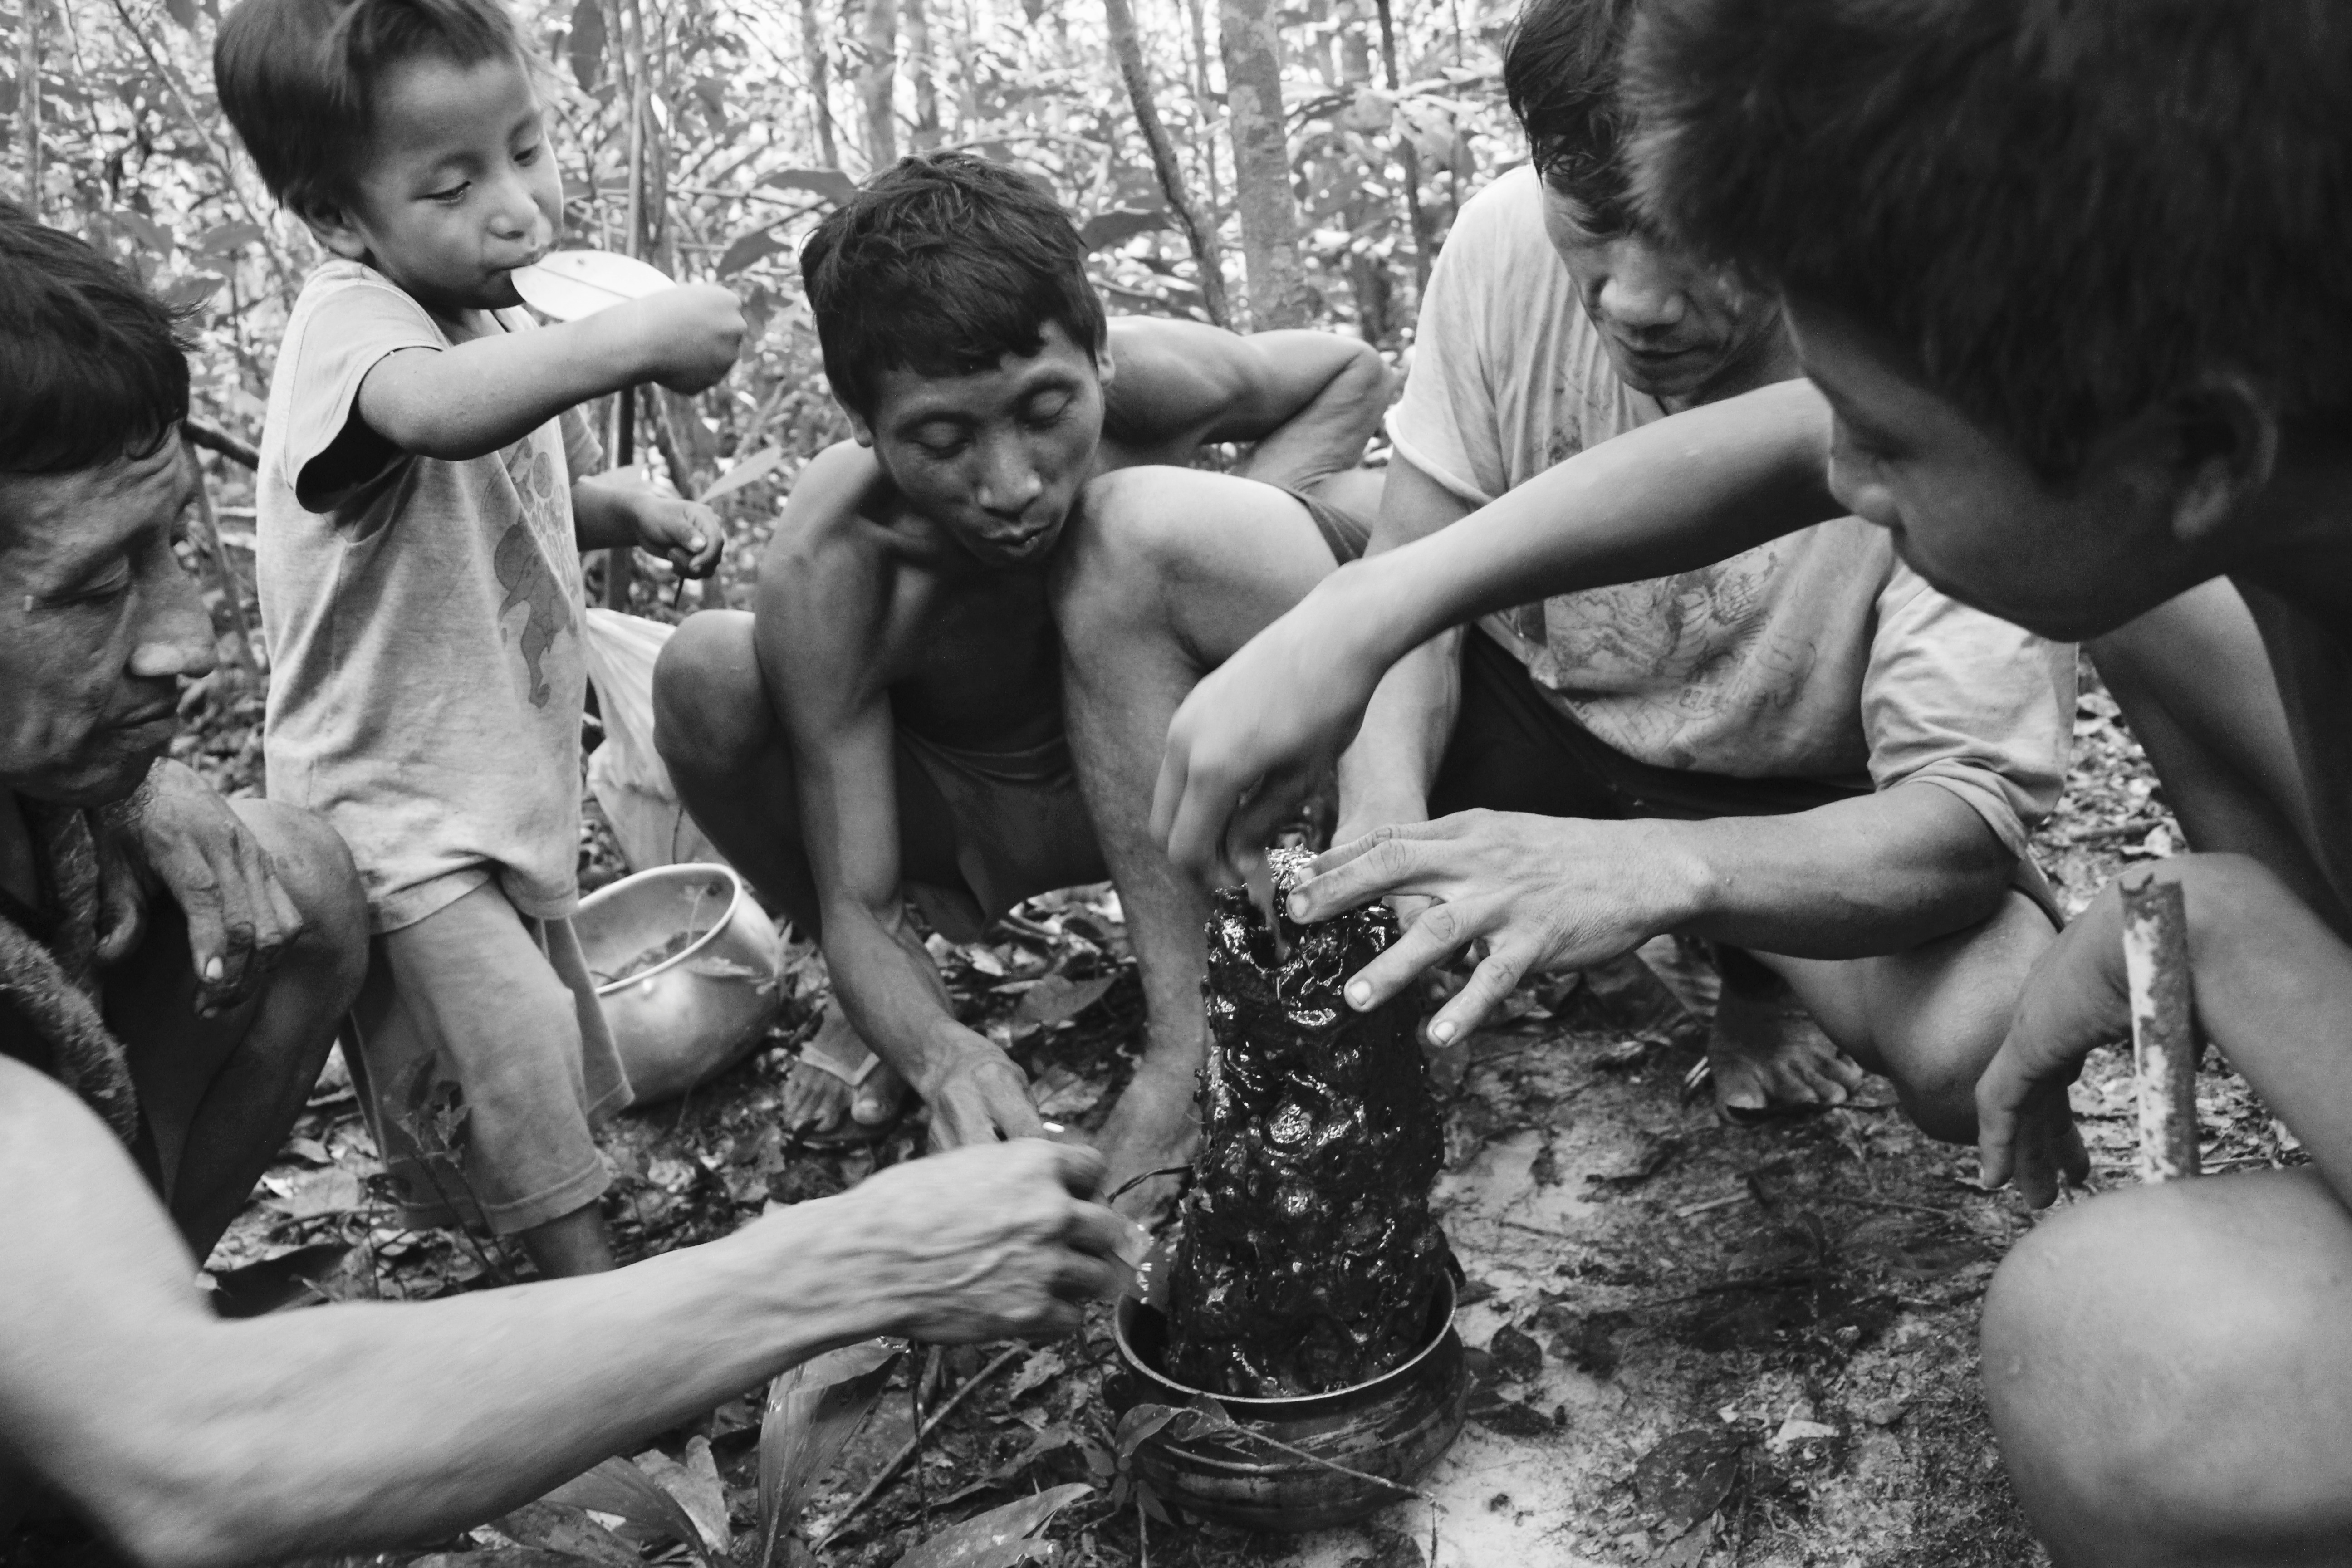
\includegraphics[width=\textwidth]{./imgs/IMG_1672}
%\caption{Takamỹxa'a, seu filho Warara’ia com a folha de mel na boca, Majhuxa’a, Hajkaramykỹa e seu filho Warajua se refastelando de \emph{hairaxĩa}, o mel da tartaruga capininga (acampamento de caça, aldeia Awá, 2013).}
%\end{figure}

Não apenas com alguns tipos de mel, mas com vários alimentos
(\emph{hanimiũ'a} ``minha comida''), as pessoas desenvolvem um elaborado
sistema de controle. Isso sucede sobretudo durante o pós"-nascimento de
crianças (\emph{wehẽ} ``sair''), menstruação, além de momentos como luto
ou doenças, que exigem atenção redobrada. As pessoas próximas (uma
família, por exemplo) se conectam de maneira consubstanciada, e a saúde
de um afeta diretamente a saúde de outro --- não muito diferente do que o
ocidente argumenta sobre os efeitos de um vírus, como o da gripe, ao
atingir um membro da família, com a potencial contaminação da família
inteira.

Os Guajá dizem não saber comer alimento ``amargo'' (\emph{irawahy}), cujo
amargor quase sempre terá fins medicinais. Apesar de gostos azedos
(\emph{hajahy}) figurarem na dieta Guajá, ainda não ``aprenderam'' a comer
amargo, como disse um amigo certa vez, ao explicar"-me a intolerância a
esse sabor. Dos procedimentos para proteger a pessoa em situações
sensíveis, como das mulheres em menstruação (``estar sangrando'',
\emph{hawy}), a ingestão de uma infusão amaríssima feita com a casca de
uma árvore chamada \emph{mata'ya} (que não identifiquei) é muito
indicada por proteger as ``tripas'' (intestinos e, nesse caso, também
fígado). Por exemplo, na primeira menstruação (\emph{hawy}
\emph{mutuhũ}, ``primeiro sangue''), a jovem deve tomar \emph{mata'ya}
para proteger o fígado e não passar mal com os alimentos. Miúdos em
geral, como fígado, vísceras e outros, estão proibidos. As mesmas
restrições alimentares recaem sobre mulheres menstruadas, além de homens
e mulheres em resguardo pós"-nascimento. Vejamos alguns desses alimentos.

%\begin{longtable}[]{@{}l@{}}
%\toprule
%\begin{minipage}[b]{0.97\columnwidth}\raggedright
%\textbf{Principais alimentos proibidos a (1) mulheres menstruadas; }%

%\textbf{(2) mulheres e homens em resguardo pós-nascimento }\strut
%\end{minipage}\tabularnewline
%\midrule
%\endhead
%\begin{minipage}[t]{0.97\columnwidth}\raggedright
%1) ovos de jaboti (\emph{kamixa ripiakera})%

%2) ovos de jacaré (\emph{jakare ripiakera})%

%3) jaboti fêmea (o macho pode)%

%4) carne de jacaré%

%5) peixe surubim%

%6) piranha%

%7) peixe curimatá%

%8) peixe traíra%

%9) fígado e vísceras em geral%

%10) macacos adultos%

%11) paca%

%12) queixada%

%13) aves "galináces" como jacamin, inhambu e mutum%

%14) veado mateiro (arapaha)%

%15) veado foboca (\emph{arapaha'ia})%

%16) pequiá, ou pequi (\emph{Caryocar villosum}) (\emph{myky'a})%

%17) pelo menos seis tipos de mel\strut
%\end{minipage}\tabularnewline
%\bottomrule
%\end{longtable}

\begin{table}[H]
\centering
%\caption{My caption}
\label{my-label}
\begin{tabular}{|l|}
\hline
\textbf{\begin{tabular}[c]{@{}l@{}}Principais alimentos proibidos a (1) mulheres menstruadas; \\ (2) mulheres e homens em resguardo pós-nascimento\end{tabular}}                                                                                                                                                                                                                                                                                                                                                                                    \\ \hline
\begin{tabular}[c]{@{}l@{}}\smallskip 1) ovos de jaboti (\emph{kamixa ripiakera})\\ \smallskip  2) ovos de jacaré (\emph{jakare ripiakera})\\ \smallskip  3) jaboti fêmea (o macho pode)\\ \smallskip 4) carne de jacaré\\ \smallskip 5) peixe surubim\\ \smallskip 6) piranha\\ \smallskip 7) peixe curimatá\\ \smallskip 8) peixe traíra\\ \smallskip 9) fígado e vísceras em geral\\ \smallskip 10) macacos adultos \\ \smallskip 11) paca\\ \smallskip 12) queixada\\ \smallskip 13) aves ``galináces'' como jacamin, inhambu e mutum\\ \smallskip 14) veado mateiro (arapaha)\\ \smallskip 15) veado foboca (\emph{arapaha'ia})\\ \smallskip 16) pequiá, ou pequi (\emph{Caryocar villosum}) (\emph{myky'a})\\ \smallskip 17) pelo menos seis tipos de mel\end{tabular} \\ \hline
\end{tabular}
\end{table}

Quando nasce um filho, nem o marido nem a esposa podem beber água por
uns dias, e o mesmo ocorre com a mulher menstruada. Só é permitido beber
\emph{mata'ya}, essa infusão de madeira amarga, e deve"-se dormir
bastante. Por isso o resguardo é chamado de ``o descanso das pessoas''
(\emph{awa nypyate hakeri}). Até o cordão umbilical cair não se come
praticamente nada, e toda a dieta deve ser observada após a queda do
``umbigo'' (\emph{iporowãena}). Pequenos peixes como mandi e sardinhas são
indicados, assim como a carne de animais pequenos, como as cotias. Nesta
época, a carne de macaco, alimento muito apreciado, só pode ser
consumida se for de animais jovens, preferencialmente de capelães.
Frutos como inajá, bacaba, açaí, cupuaçu, bacuri e cacau podem ser
consumidos, bem como animais como a cotia e o tatu. O tatu, inclusive,
tem uma carne indicada para consumo em períodos de fraqueza pois, assim
como o couro do tatu é duro, sua carne fornece força e dureza
(\emph{hatỹ}) para quem a come. Nesses períodos só se podem consumir
jabotis machos, já que um dos riscos mínimos da mulher que ingere carne
de jaboti fêmea seria dar à luz filhos com problemas de pele, e o risco
máximo seria dar à luz jabotis. Para a proibição do consumo de diversos
alimentos, os Guajá dão explicações relacionadas aos possíveis efeitos
negativos no corpo do bebê ou dos pais. Peixes como o curimatá
(\emph{mykukyruhua}) e a traíra (\emph{tara'yruhua}) devem ser evitados,
pois podem gerar feridas no corpo da criança. A carne de ``jabotas'' ---
as jabotis"-fêmeas ---, por exemplo, é lembrada por produzir cansaço nos
homens, que não aguentariam subir as ladeiras da mata. Nesta época só
comem jabotis machos.

Quanto às dezenas de méis que ainda veremos neste livro, adianto que
eles são alimentos muito apreciados e amplamente consumidos, mas podem
ser também muito perigosos. Os méis em geral são alimentos ``quentes'' que
causam \emph{emoção} a quem consome. Sua doçura faz bem à saúde, mas
algumas espécies podem ser nocivas em períodos de resguardo.

%\begin{longtable}[]{@{}l@{}}
%\toprule
%\begin{minipage}[b]{0.97\columnwidth}\raggedright
%\textbf{Méis interditos na \emph{couvade}}%

%\textbf{nome do mel → efeitos}\strut
%\end{minipage}\tabularnewline
%\midrule
%\endhead
%\begin{minipage}[t]{0.97\columnwidth}\raggedright
%\emph{iramuira} - mel do inhambu → febre%

%\emph{kamixaira} - mel do jaboti → coceira no corpo%

%\emph{mu'uira} → atrofia nos dedos das mãos e pés%

%\emph{tataira} - abelha caga-fogo%

%\emph{Oxytrigona tataira tataíra})→ queima a pele da criança%

%\emph{pirairuhua} → causa calafrios em pais e filhos%

%\emph{uhua} - mel da anta/abelha "xupé"%

%(\emph{trigona hyalinata Lepeletier}) → não identificado\strut
%\end{minipage}\tabularnewline
%\bottomrule
%\end{longtable}

\begin{table}[!ht]
\centering
%\scriptsize
\label{my-label}
\begin{tabular}{|l|}
\hline
\multicolumn{1}{|c|}{\textbf{\begin{tabular}[c]{@{}c@{}}Méis interditos na couvade\\ nome do mel → efeitos\end{tabular}}}                                                                                                                                                                                                                                                                                        \\ \hline
\begin{tabular}[c]{@{}l@{}}\emph{iramuira} - mel do inhambu → febre\\ \\ \emph{kamixaira} - mel do jaboti → coceira no corpo\\ \\ \emph{mu'uira} → atrofia nos dedos das mãos e pés\\ \\ \emph{tataira} - abelha caga-fogo\\ (\emph{Oxytrigona tataira tataíra}) → queima a pele da criança\\ \\ \emph{pirairuhua} → causa calafrios em pais e filhos\\ \\ \emph{uhua} - mel da anta/abelha ``xupé'' \\ (\emph{trigona hyalinata Lepeletier}) → não identificado\end{tabular} \\ \hline
\end{tabular}
\end{table}

O consumo do mel \emph{iramuira} (mel do inhambu) para a mulher
menstruada ou em cuidados pós"-parto provocaria o endurecimento de seu
intestino. Hajkaramykỹa me contou sobre uma mulher no passado que comeu
desse mel enquanto estava menstruada, e seus órgãos internos, o
intestino em particular, ``secaram''. Ela ficou entupida sem conseguir
urinar ou defecar e morreu.

No caso de um resguardo menor, por menstruação, os cuidados não recaem
no marido e filhos. Veremos ainda que os Guajá compartilham a
paternidade, pelo que crianças têm mais do que um \emph{pai}, e os
cuidados pós"-nascimento --- todo o sistema de \emph{resguardos} que
restringe a alimentação e atividades --- recaem não somente sobre o marido
da mãe, mas sobre todos os outros que são considerados genitores da
criança e, muitas vezes, os irmãos do pai (\textsc{fb}). Embora as mulheres
experimentem essas interdições de maneira periódica --- mensalmente, os
homens, por sua vez e apesar de bem menos, as experimentam não só quando
nascem seus filhos com sua esposa, mas qualquer outra criança que ele
tenha ajudado a conceber.

Em geral, não há consumo de carne que fique impune. Nesses períodos os
homens sequer devem sair para caçar, e nem homens nem mulheres devem
mexer com caça no sentido de ``limpar'' (\emph{hape}) o animal: despelar,
tirar vísceras, cortar, cozinhar. O resultado imediato são dores de
cabeça (\emph{jakỹ wakyhy ta}) e febre em pais e filhos. A mesma dor de
cabeça ocorre se qualquer um da família consumir macacos adultos. Todas
as atividades de caça são interrompidas, e um homem só poderá abrir
exceção, sob muito cuidado, caso tenha outras bocas para alimentar --- se
seus filhos estiverem com fome. Diversos animais podem ser capturados
enquanto o bebê não ``mexer o pescoço'' com autonomia (não estiver
ereto), tais como veado"-mateiro e veado"-foboca. Ainda assim, por
exemplo, não se matam machos das espécies macaco"-prego, cairara, ou
quatis, pois provocam até enlouquecimento. Mesmo as fêmeas não são
consumidas, são capturadas apenas para aplacar a fome das crianças.

Seja na \emph{couvade} ou fora dela, comer carne (\emph{ha'okera}) é
algo sempre perigoso --- devido a ``raivas'' e vinganças que os animais
podem lançar sobre quem os caçou ---, e alguns animais em particular são
perigosos sempre, como parece ser o caso do veado mateiro
(\emph{arapaha}). Carnes como a de veado, apesar de amplamente
consumidas, sempre provocam revertérios por serem ruins, ``reimosas'',
\emph{manahỹ}. Quando a mulher de Tatuxa'a deu à luz a pequena
\emph{Iwapanỹ}, ele foi caçar (esperar) um veado mateiro na floresta,
sem que o cordão umbilical da menina ainda tivesse caído. Ele o fez,
pois seu outro filho, Takwarary, estava ``chorando de fome'', pedindo"-lhe
carne para comer, e os homens Guajá sempre vão caçar quando seus filhos
estão clamando por comida. Por isso ele resolveu ``esperar''
(\emph{matakwa}) o veado à noite. Sua caçada foi bem"-sucedida, ele
conseguiu matar três cotias a caminho da espera e um veado mateiro
durante a noite. No dia seguinte retornou à aldeia, e no mesmo dia sua
filha recém"-nascida contraiu uma febre alta que não passava. Tiveram que
retirá"-la da aldeia com o carro da \textsc{sesai} e enviá"-la para o hospital na
cidade de Santa Inês. Segundo Tatuxa'a, sua filha quase morreu. Além de
atribuir a doença da filha recém"-nascida ao fato de ter ido caçar veados
no momento que deveria estar descansando em casa, o homem também
comentou que, se tivesse matado uma onça, certamente sua filha estaria
morta hoje.

A onça é um animal perigoso de matar. Os Guajá gostam da carne de
suçuarana (onça parda); lembra"-lhes o sabor da carne de veado. E mesmo a
onça pintada podia ser consumida, ao menos ``antigamente'', lembram as
pessoas. Porém, de todas as restrições em período de cuidados
pós"-nascimento (mas também menstruação e doenças), não se deve matar, e
muito menos consumir, carne de suçuarana (ou qualquer outra onça), pois
provocará a morte do bebê. No caso da onça, a proibição de matar se
inicia na gravidez e segue até o pós"-parto. Caso um homem mate o felino
durante esse período, além da morte do bebê, a própria grávida ou mãe
poder morrer ou seu leite secar. O seio da esposa pode sumir, tornando"-a
``lisa'', ``como se tivesse o peito de um homem'', alertou"-me certa vez
Hajkaramykỹa. Em um relato de seus diários de campo, a pesquisadora Rosana Diniz escreve:

\begin{quote}
\emph{Nesse sentido, Hajmakoma'ã me fez o seguinte relato, em 2010: tinha ido
caçar e encontrou com uma onça, mas esta o viu primeiro. Então, ele se
pôs a correr na floresta, e a onça atrás. Chegando em um rio, ele
jogou"-se na água e a onça, então, desistiu da perseguição. E porque você
não atirou nela? Perguntei. Ele respondeu: E minha filha pequena,
\emph{xikari} (minha irmã)? Não posso matar onça, faz mal para a minha
filha, ela pode morrer (Diniz, 2015, pp. 55--56).}
\end{quote}

A quebra do resguardo de nascimento, de acordo com Hajkaramykỹa, atinge
a todos da casa, e por determinados animais, caso das onças, a escolha
em caçar e/ou comer pode ser mortal. Pai, mãe, filhos, irmãos e pessoas
ligadas à casa estão relacionados e, por sua vez, se conectam a
diferentes subjetividades (animais, vegetais ou espectrais) que vivam na
floresta. Por isso, vômitos e fezes dos bebês não podem ser abandonados
nem no chão da aldeia (pois são comidos por cachorros) nem na floresta,
pois são comida de animais, principalmente os gambás, jabutis,
carrapatos e marimbondos, sob o risco de adoecimento ou morte do bebê.
Esses excrementos --- para não ser consumidos por animais --- também não
podem ser enterrados para não virarem ``comida de minhoca''. Caso as
minhocas (\emph{amirikuria}) --- ou qualquer outro animal --- o comam, os
bebês adoecem. O tratamento mais comum é envelopar essas fezes em folhas
(como a folha de \emph{akareho}, por serem planas) e a amarrar com
cipozinhos (como pedacinhos de ``cipó titica'' por exemplo) deixando
pendurados em alguma árvore, livre do alcance de todos os bichos. Esses
``embrulhos'' são chamados \emph{ximixia}. Não podem ser jogados fora,
nem enterrados. Devem ficar pendurados até as fezes apodrecerem
(\emph{ipiru} ``podre'').

%\textbf{Foto de ximixia}
%\begin{figure}[H]
%\centering
%  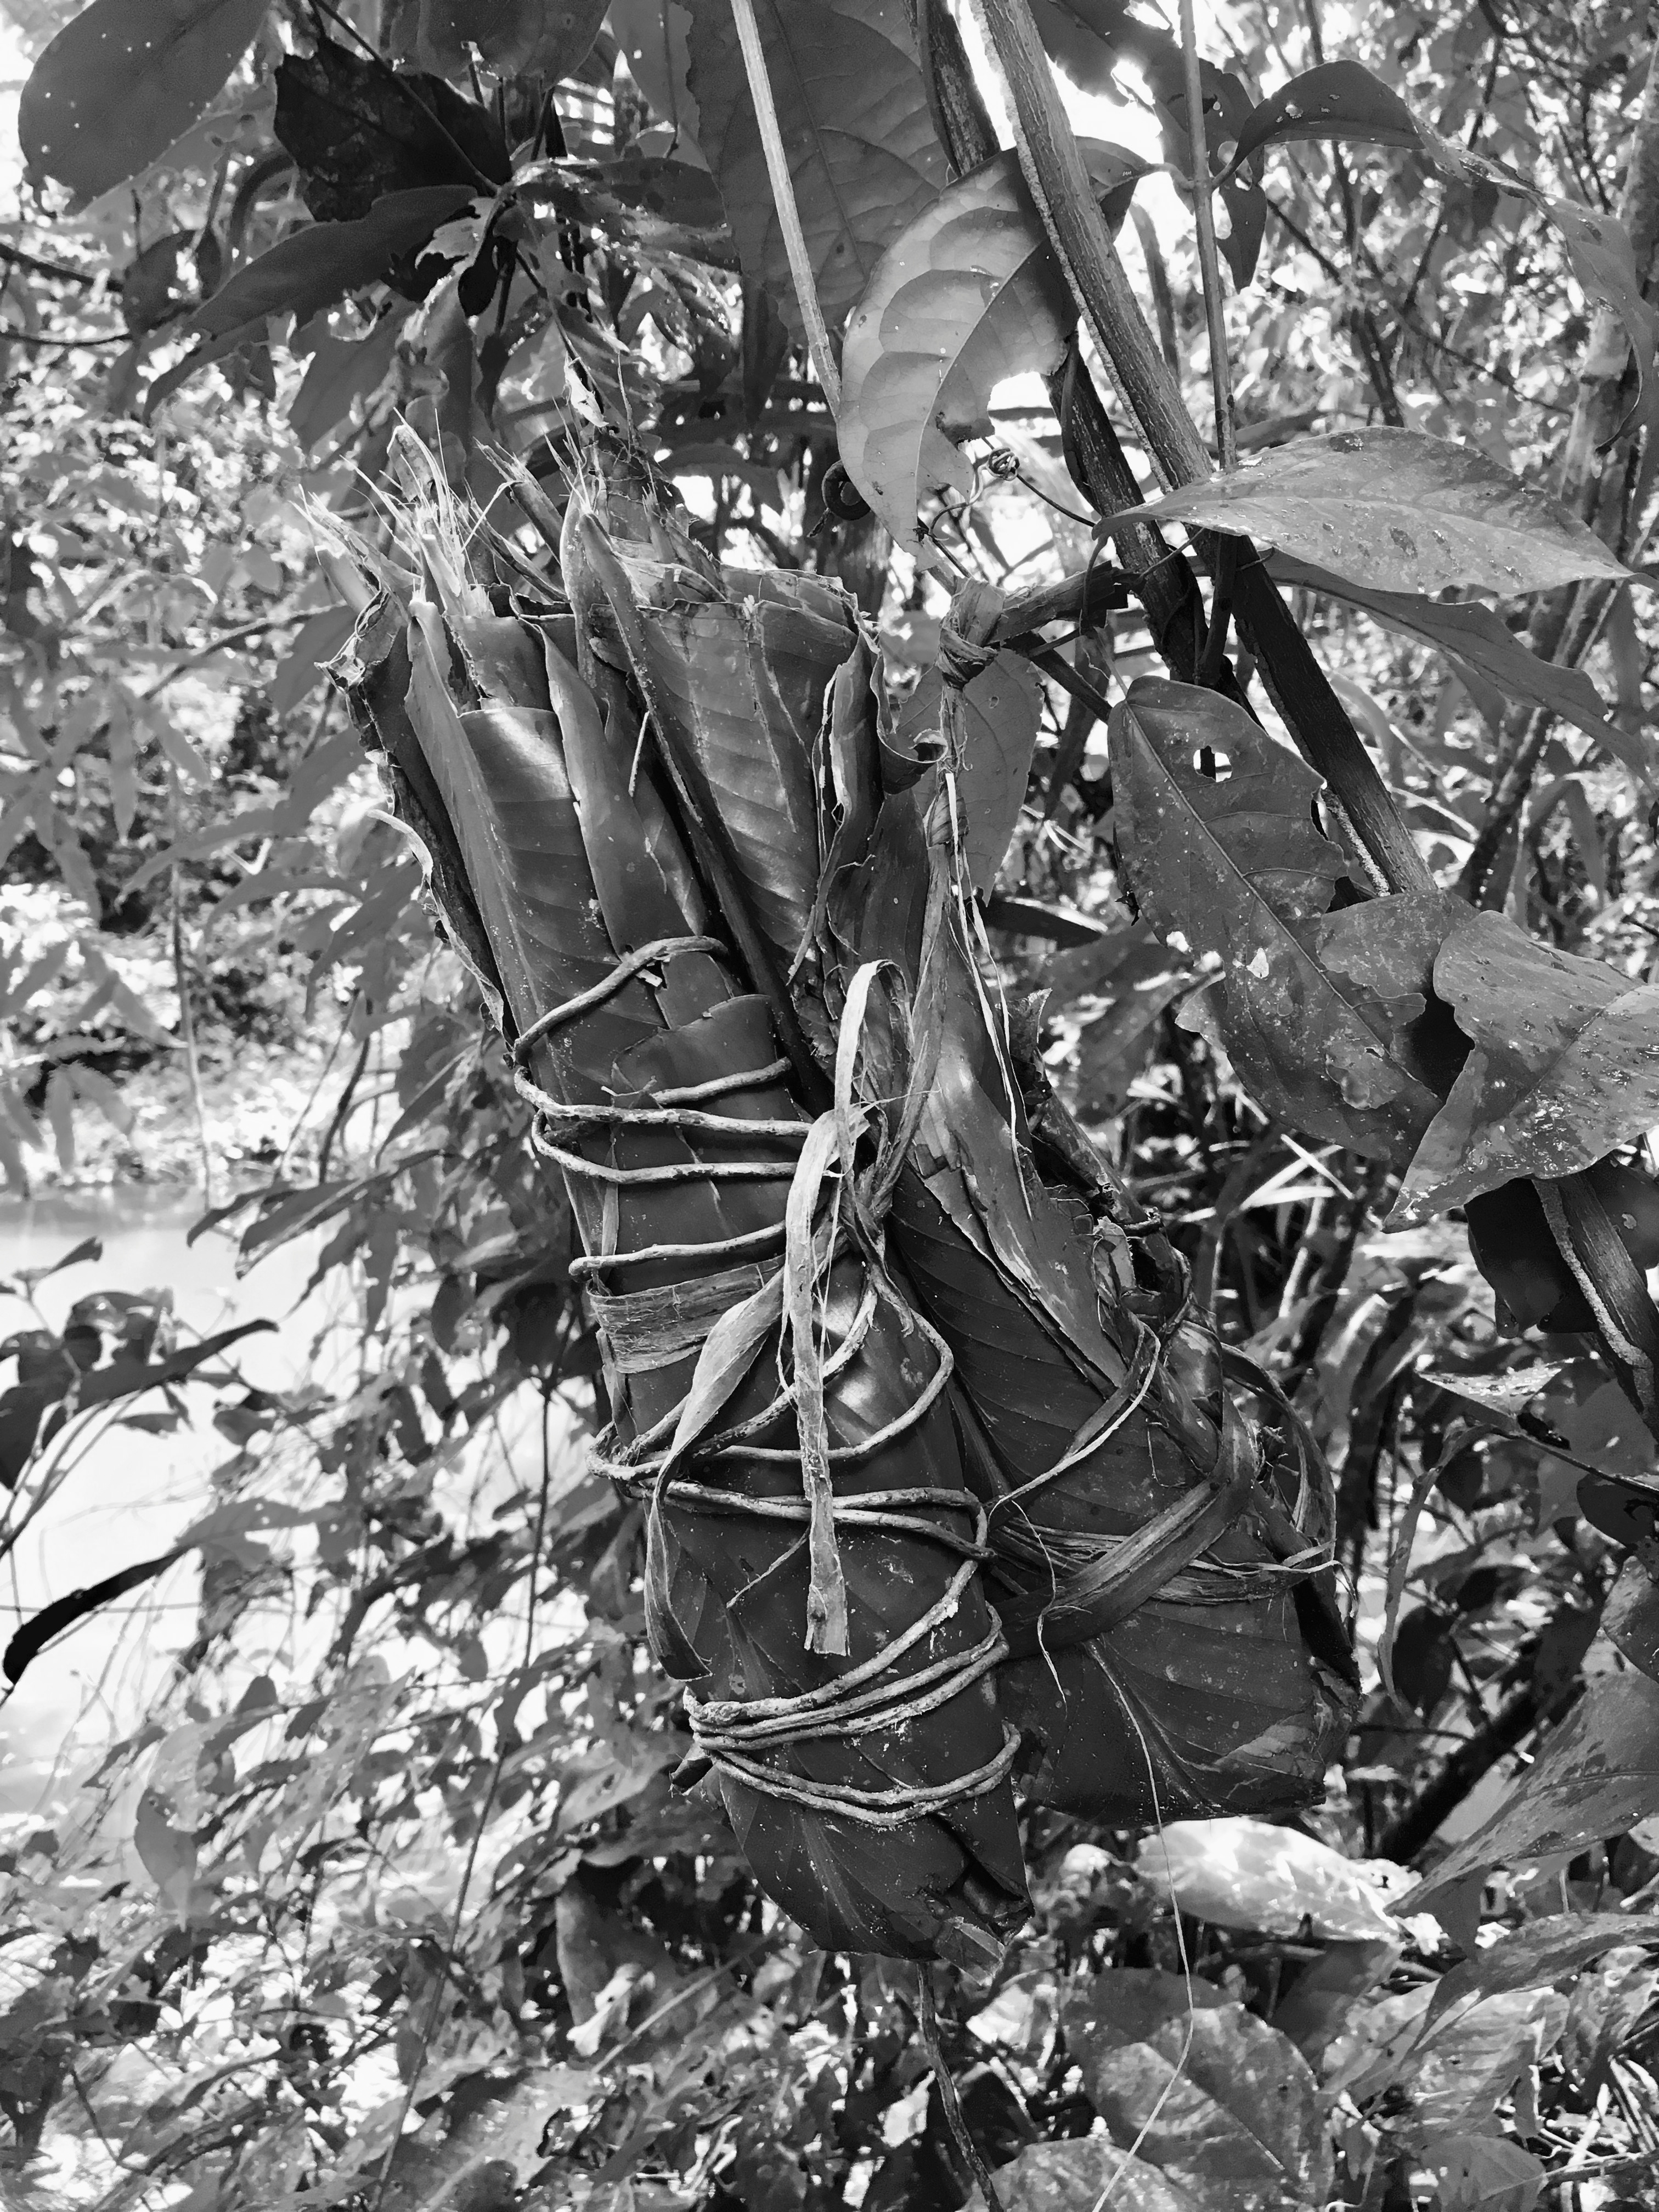
\includegraphics[width=\textwidth]{./imgs/IMG_4613}
%\caption{Ximixia feita por Jawatara'ia e pendurada no caminho da aldeia após o nascimento do seu filho (aldeia Juriti, 2018).}
%\end{figure}

Diversos cuidados também devem ser observados no manuseio dos alimentos.
Apenas como um exemplo, ossos de machos de espécies de macacos como o
cairara (\emph{Cebus kaapori}) e macaco"-prego (\emph{Cebus apela}) não
devem ser atirados no chão para que não entrem em contato com ninguém.
Em se tratando desses ossos, o perigo é algo próximo da feitiçaria
(chamada pelos Guajá de \emph{ma'akwá}). Os ossos de fêmea, porém, não
carregam feitiço. Ao consumir macacos desse tipo, seus ossos devem ser
separados da carne antes de os pais os darem aos filhos, para que as
crianças não os arremessem em alguém ou algum lugar.

Por outro lado, apesar de mencionar aqui a ideia de ``regras'' e
cuidados, da forma pela qual esses resguardos são pensados, as pessoas
nunca falam em interdições (e muito menos regras) propriamente. Se
existem resguardos, é porque também existe uma possibilidade real, um
desejo em sair para caçar, seja para matar a fome (\emph{nahakatãj}) dos
filhos maiores ou outros parentes, seja para acompanhar os amigos por
pura vontade de matar bichos. É muito comum pessoas ligadas ao pai em
resguardo chamarem"-no para caçar, insistindo até para ele descumprir seu
período de reclusão. Este quase sempre deve dizer que ``está cansado para
caçar'' ou ``tem que ficar com seu filho'' ou mesmo que ``sua mulher não
quer ficar sozinha''. Mesmo em mudança na alimentação e nos hábitos, o
homem em reclusão não insinua isto de maneira tão explícita em suas
falas. Os argumentos evocados para ele permanecer em sua casa (ou mesmo
em sua rede) são sempre mais ``prosaicos'' do que a ideia de ``resguardo''
ou ``regras''. Preferem dizer: ``Vou ficar em casa olhando meu filho!'', e
essa frase resumiria tudo.

Por fim, podemos pensar que as proibições e interdições de dieta para as
mulheres e homens que esperam ou tiveram filhos recentemente só são
realmente conhecidas por seus efeitos, como já discutido por Coelho de
Souza (2004, p. 44), apesar de todos os \emph{a priori} que enumerei
acima. Por exemplo, as mulheres da aldeia Juriti não comiam carne de
veados (mateiro e foboca) e galinha ou frango, sob o risco de terem
fortes sangramentos. Apenas nos últimos anos (2011/2012), quando pessoas
de outras aldeias --- cujas mulheres consomem carne de veado --- começaram a
manter contatos mais intensos com os Guajá da aldeia Juriti, elas
passaram a comer carne de veado (caso não estejam menstruadas) e, de
maneira geral, tal ``proibição'' caiu. Nas viagens para a cidade em
reuniões e encontros, que são cada vez mais frequentes na vida dos
Guajá, a observação dessas regras é motivo de debates entre maridos e
esposas. Certa vez, Jauxika, que estava grávida de oito meses, proibiu
seu marido Takwari --- que estava indo para uma reunião em outra aldeia ---
de comer carne de frango, até que o pai de Takwari, Pira'ima'ã,
interveio e disse que quando sua esposa esteve grávida e ele foi à
cidade, comeu carne de frango, e nada de mal aconteceu a ele. Jauxika, a
mulher, ouviu com interesse a explicação do homem e então disse para
Takwari que ele podia, sim, comer carne de frango e gado, mas devia
prestar atenção para não passar mal. Mas que não comesse, de forma
alguma, carne de porco (do mato ou dos brancos), pois isso faria mal a
ela e ao bebê. Os alimentos específicos que podem ou não ser consumidos
são sempre debatidos a cada nova gravidez, a cada nova situação de
restrição. Ainda que haja esse conjunto que aqui destaco e costuma
sempre ser observado, as interdições sempre serão compreendidas pelos
efeitos e resultados de determinados alimentos no corpo dos sujeitos,
seja uma pessoa ou uma família com que se afetam mutuamente.

Embora não seja meu tema de pesquisa, finalizo este tópico anotando que
os Guajá desenvolveram uma infinidade de medicamentos
(\emph{pohỹ})\footnote{Também denominados \emph{ira pohỹ}, ``remédio das
  árvores''.} muito eficientes no combate a muitas doenças\footnote{Ver o
  artigo de Cormier (2005) em que a autora traça um perfil mais
  detalhado daquilo que ela denomina ``simbolismo vegetal'' dos Guajá,
  apresentando um conjunto bem mais amplo de doenças e relacionando"-as à
  concepção Guajá de pessoa e morte. Ainda no tratamento da etnobotânica
  dos Guajá, o trabalho de Balée (1994) é sem precedentes.}. Mesmo
guardando um grande fascínio pela etnomedicina dos \emph{karaia}, com
seus comprimidos, pomadas e injeções (a que recorrem sistematicamente),
os Guajá fazem uso de ambos os remédios (dos \emph{awa} e dos
\emph{karaia}) em diversas situações. Por exemplo, quando o rapaz Juxa'a
foi picado por uma cascavel e, na enfermaria do \textsc{pin}, lhe aplicaram
algumas doses de soro antibotrópico, sua mãe aplicou"-lhe em cima da
picada um emplastro feito com uma casca de árvore chamada
\emph{hiratanỹ} a fim de expulsar o veneno da cobra. Muitas dessas
folhas, cascas e cipós têm nomes de animais que são seus \emph{jara}
(``donos''). Vejamos alguns desses medicamentos. Para salvaguardar a
propriedade e o conhecimento sobre essas plantas, omito os nomes nativos
substituindo"-os por ``\textsc{p}'', de planta, seguido de um número:

\emph{\textsc{p}1} --- Folha que se amassa a fim de tratar dores
musculares, dentre outras dores. Passa"-se nos braços e articulações, em
aplicações periódicas, e é capaz de expulsar tais dores. Também
utilizada contra febre, pode ser ingerida após macerada (\emph{jamixo})
e adicionada a água e mel.

\emph{\textsc{p}2} --- (algo que pode ser traduzido como ``veado vegetal'')
--- Folha que os Guajá esquentam na fumaça do moquém, colocando"-a em
seguida nas pernas, nádegas e costas para debelar a febre. Um
antitérmico.

\emph{\textsc{p}3} --- Com muitas utilidades, esta entrecasca também é
chamada \emph{irawahy} (``amargosa''), e tem como função tratar dores no
fígado, estômago e vísceras. Pode ser utilizada em forma tópica,
colocada sobre o abdômen da pessoa em repouso. Se o enfermo tiver
vômitos, é ingerida macerada misturada com mel e água, de modo a
amenizar o gosto amargo. Após o nascimento de uma criança, seu pai deve
ingeri"-la macerada, com a finalidade de proteger seu fígado.

\emph{\textsc{p}4} --- Utilizada contra dores de cabeça, esta folha é
muito cheirosa. Se macerada, pode ser aplicada durante os banhos no rio.
Após alguns dias de aplicação a dor se esvai.

\emph{\textsc{p}5} --- De função idêntica à \emph{Henemy ka'y}.

\emph{\textsc{p}6} --- (uma tradução possível é ``mel vegetal'') --- Folha de
cheiro agradabilíssimo, cuja função é espantar dores de cabeça e no
corpo. Utiliza"-se esfregando"-a nas partes afetadas.

\emph{\textsc{p}7} --- De uso e função parecida da \emph{Haira Ka'a},
porém só aplicável a dores de cabeça.

\emph{\textsc{p}8} --- Entrecasca de uma árvore cuja seiva alivia as dores
de ferida e queimaduras, além de ajudar na cicatrização de ferimentos
externos.

\emph{\textsc{p}9} --- Folha utilizada contra a febre. Utiliza"-se
esfregando"-a no corpo.

\emph{\textsc{p}10} --- Frutinha cheirosa de cor amarela, de uso tópico;
esfregam"-na no corpo a fim de expulsar dores e febre.

\emph{\textsc{p}11} --- Casca de uma árvore, com o mesmo nome. Se inalada,
seu cheiro mentolado combate febre e calafrios.

Esta é uma pequena amostragem de medicamentos que atuam contra as
doenças que atacam o \emph{hajtekera} e, por consequência, os
componentes vitais de uma pessoa (para uma boa análise da etnomedicina
Guajá, consultar Cormier, 2005).

\section{\emph{Ha'aera} e \emph{Ajỹ}, morte e fúria}

O último elemento constituinte da pessoa Guajá, que apresento aqui, é o
\emph{ha'aera}\footnote{O termo correto é -\emph{a'a}; \emph{h-a'a-er-a}
  é o resultado da junção do prefixo de 3ª pessoa \emph{h-} +
  ``espectro/raiva'' \emph{a'a} + sufixo de a.n. retrospectiva -\emph{er} + sufixo nominal -\emph{a}; porém os Guajá nunca se referem a
  \emph{ha'aera} como \emph{a'a}, sempre o fazem utilizando o sufixo -\emph{era}
  ou -\emph{e}, nas formas \emph{ha'aera} ou \emph{ha'ae} (a depender da
  construção da frase).}. Os Guajá traduzem tal palavra para o português
por ``raiva'', não se tratando da mesma ``raiva'' expressa pelo termo
\emph{imahy}. \emph{Imahy} é um sentimento que, apesar de perigoso e
desprezado, é muito comum e desejável em diversas situações, como na
guerra. \emph{Ha'aera} pode ser traduzido pela ideia de
``raiva"-espectro'', devido tanto à sua condição de ``sombra/alma'' bestial,
liberada após a morte (processo cuja consequência é a transformação em
um ser que é pura ``raiva'', os \emph{ajỹ}), pelo fato de o \emph{ha'aera}
atuar durante a vida como um dos componentes da pessoa humana. Para
melhor definição do termo, podemos contrastar o \emph{ha'aera} com o
\emph{hajtekera}, sendo este último um princípio que agencia a vida,
enquanto o \emph{ha'aera} agencia morte, dores e sofrimentos.

O \emph{ha'aera} é uma substância constitutiva do próprio ser: ``Está por
aqui!'', me disse certa vez Wiraho, apontando para seu peito e barriga.
Humanos e alguns animais possuem \emph{ha'aera}. E no caso dos animais é
essa potência que atormenta os humanos na forma de vingança após as
caçadas --- a qual emana doenças e retira a sorte em caçadas futuras. No
caso particular da constituição da pessoa, o \emph{ha'aera} é aquilo que
diversos autores chamariam de ``espectro'' de um morto (ver \emph{Jurupari
-} Waiãpi, Gallois, 1988, p. 178). Uma vez morta, as partes da pessoa se
desfazem: o \emph{ipirera} apodrece na terra; o \emph{hajtekera} se
encaminha para o \emph{iwa}; e o \emph{ha'aera} se transmuta em
\emph{ajỹ}.

O \emph{ha'aera} não é só o espectro de um morto recente, uma sombra da
pessoa morta que um dia se transformará em \emph{ajỹ}, ele é uma
substância que também compõe a vida e que só após a morte vaga como
``alma penada'' e se mescla à massa de seres \emph{ajỹ}, que são
dependentes do \emph{ha'aera} para viver. Não é possível afirmar que o
\emph{ha'aera} tenha uma aparência. Ao contrário, os Guajá definem
literalmente como uma substância, algo espectral. ``É como o seu
repelente!'', me disseram certa vez, um agente que tem poder de
penetração tão capilar como um gás. É algo que todo humano carrega, pois
faz parte da composição física humana, porém, liberado violentamente
após a morte, funcionando como uma energia formadora de seres ligados à
morte, os \emph{ajỹ}. A constante ameaça aos humanos que emana dos
\emph{ajỹ} é dita como \emph{ajỹ} \emph{ha'aera}, já que os \emph{ajỹ}
dominam esse princípio mortal, lançam"-nos nos humanos fazendo"-os adoecer
e até morrer. Os \emph{ajỹ} são constituídos pelo \emph{ha'aera} de
ex"-humanos, por isso mesmo, em diversas situações, podem simplesmente
ser denominados \emph{ha'aera}, tal como um sinônimo. O \emph{ha'aera}
também pode ser chamado de \emph{ajỹ karawara}, já que os \emph{ajỹ} a
manipulam da mesma forma que os homens Guajá fazem com os
\emph{karawa(ra)}, as potências celestes que auxiliam os humanos em suas
curas. Em outras palavras, o \emph{ha'aera} é o \emph{karawara} dos
\emph{ajỹ}. Seres como os \emph{ajỹ} talvez sejam dos que mais
apareceram nas etnografias Tupi"-Guarani desde os primeiros relatos de
viajantes, e permanecem como tópico importante até os trabalhos
atuais\footnote{Para um balanço comparativo de noções parecidas a essa,
  como \emph{Anhang}, \emph{Aignan}, \emph{Anhanga}, dentre outras, cuja
  precedência na literatura etnológica é ampla, ver Viveiros de Castro
  (1986, p. 255).}. Porém, vejamos o que os Guajá têm a dizer sobre
eles.

``Seres pequenos, com a estatura de crianças e muito feios!'' Essa é uma
das formas de definir os \emph{ajỹ}, entidades que habitam antigos
acampamentos, ocos de árvores, buracos e áreas escuras da floresta. São
capazes de tirar a vida de alguém com um simples toque. Somente por
pressenti"-los, uma pessoa pode entrar em estado febril. Da mesma forma,
são como ``curupiras'', que atrapalham cotidianamente a vida dos
caçadores, provocam doenças, mortes, além de serem \emph{jara} (``donos'',
``controladores'') de um expressivo número de animais. Os Guajá atribuem
muitas de suas desventuras e azares na caça (\emph{panemuhũ}) aos
\emph{ajỹ}. Diferentemente dos Ka'apor ou dos Araweté, as figuras do
\emph{koropí} (Viveiros de Castro, 1986, p. 244) ou \emph{curupir}
(Huxley, \emph{op. cit.}, p. 205) estão ausentes do mundo \emph{awa}; são os
\emph{ajỹ} que desempenham esse papel de seres controladores de alguns
animais de caça, capazes, inclusive, de perseguir um caçador
lançando"-lhe \emph{ha'aera} e deixando"-o \emph{panemuhũ} (``panema'', sem
sorte), como veremos mais à frente. Os Guajá recolocam a figura
Tupi"-Guarani do \emph{curupira} (com suas formas e atitudes específicas)
nos \emph{ajỹ}: aparência feia, monstruosa; domínio sobre algumas
espécies animais; hábitos noturnos; ataque a caçadores, dentre outras.
Isso pode ser atestado ao observarmos o caso Waiãpi, em que o
\emph{kurupi} ou \emph{kurupira}, embora seja entidade ligada aos
\emph{añã} waiãpi, não se confunde com eles. Devido a sua feiura e dieta
canibal, o \emph{kurupi} é, nos waiãpi, associado aos \emph{añã}, também
chamado \emph{añã poro'õ} (``o maligno que nos come''), \emph{añã'go
ka'apor} (``o grande maligno da floresta'') e ainda \emph{añã Tapirã'i}
(``dono da sapopema''). De acordo com um xamã Waiãpi, ``Kurupira é a mesma
coisa que Jurupari'' (Gallois, 1988, p. 136).

Se pensarmos que o \emph{ha'aera} dos Guajá pode ser comparado ao
\emph{Jurupari} waiãpi, ao mesmo tempo que os Waiãpi põem em sinonímia o
\emph{kurupi} e os \emph{añã} (seres comparáveis aos \emph{ajỹ} Guajá),
podemos afirmar que, ao contrário desses outros povos (Araweté, Ka'apor
e Waiãpi) que convivem com a figura do \emph{curupira}, os Guajá
depositam as potencialidades deste nos \emph{ajỹ}: seres com caráter
múltiplo, de alma morta e protetor dos animais, dentre outras qualidades
possíveis. Além de provocar doenças e morte, os \emph{ajỹ} são seres com
os quais os Guajá constantemente estão sujeitos a encontrar,
principalmente porque alguns dos animais mais caçados pelos humanos são
de criação (-\emph{nima}) dos \emph{ajỹ}. São eles: o veado mateiro
(\emph{arapaha}), veado foboca (\emph{arapaha'ia}), cotia
(\emph{akwixia}), paca (\emph{kararuhua}), e o quati (\emph{kwaxia}).
Esses devem ser caçados pelos humanos com comedimento e atenção, pois
onde estão podem também estar seus ``donos'' (\emph{jara}), os \emph{ajỹ}.
Portanto, já não estamos somente no campo dos espectros e sombras
(\emph{ha'aera}), mas sim no de seres que, assim como os \emph{awa} e os
\emph{karawara} celestes, detêm recursos de ``domínios'' (\emph{riku})
sobre outros seres e se relacionam --- ainda que de forma infeliz --- com os
humanos.

Como habitantes da mata, os \emph{ajỹ} dominam uma série de seres,
situações e princípios, tornando a caçada --- para os humanos --- uma
atividade ainda mais perigosa e guerreira. Os Guajá dizem que podem
perceber a presença dos \emph{ajỹ}, pois sentem frio (\emph{haxỹ}) e
dores de cabeça quando tais seres estão próximos. Além disso, os
\emph{ajỹ} produzem um assobio longo característico (pois é o único som
que sabem emitir) e batem repetidamente no tronco das árvores com uma
grossa vara de madeira (``um pedaço de pau''), a fim de dispersar os
animais. Em uma tarde, na aldeia Juriti, um homem chamado Hajmakoma'ã me
alertou para um assobio que ouvíamos ao longe: ``Você está ouvindo esse
assobio?'' ele me perguntou, ``são os \emph{ajỹ}!'' ele mesmo respondeu.
Sem entender direito sua afirmação, interpelei"-o dizendo que se tratava
do canto de um pássaro e não do assobio dos \emph{ajỹ.} Ele concordou,
afirmando que tratava"-se do cricrió (\emph{Lipaugus vociferans}),
pássaro que é chamado ``\emph{ajỹ mixiura}'', um dos animais de criação
(-\emph{nima}) preferidos dos \emph{ajỹ}. Por isso, sempre que ouvem o
cricrió cantar, eles sabem que os \emph{ajỹ} estão por perto. O som do
cricrió é dito ser o próprio som dos \emph{ajỹ}, e este pássaro tem a
capacidade de se transformar em \emph{ajỹ}, tendo em vista que ele mesmo
o é. O mesmo ocorre com o canto do pássaro \emph{hakawỹ} (acauã -
\emph{Herpetotheres cahinnans}), um canto causador de doenças pois
contém \emph{ha'aera}. Se um caçador ouvir seja o acauã (\emph{hakawỹ})
ou o cricrió (\emph{ajỹ mixiura}) enquanto estiver na floresta, pode ser
que não encontre caça alguma, pode ser que fique com febre, pode ser que
algo ainda pior aconteça (e pode ser que nada ocorra também). Em todo o
caso, ele deve fugir para longe do alcance do canto. Da mesma forma que
o gambá (ou mucura), cujo nome na língua Guajá é \emph{ajỹ,} é um outro
(e talvez o principal) avatar dos \emph{ajỹ}. Seu cheiro fétido é o
mesmo cheiro de morte exalado pelos \emph{ajỹ}. Muitos desses animais
são pura \emph{ha'aera} e, em diversas ocasiões, são chamados
``\emph{ajỹ}'', independentemente da forma que tenham. Quanto à sua dieta,
os \emph{ajỹ} se alimentam de jaboti (\emph{kamixa}), do quelônio
capininga (\emph{jaxaihua}) e de outro tipo de tracajá chamado
\emph{marapea}. Também comem inajá (\emph{inajã}), açaí (\emph{jahara}),
bacaba (\emph{pinawã}), oiti (\emph{hixi}), além de vários frutinhos de
que os humanos não se alimentam, como a tatajuba (\emph{taryka}) e o
jatobá (\emph{itawa}), que os veados, pacas e antas comem --- pois os
\emph{ajỹ} apreciam a mesma comida que seus animais de criação.

Os \emph{ajỹ} contam com --- por assim dizer --- dois grupos de \emph{ajỹ
nima} (``animais de criação''); um deles os humanos caçam e comem;
enquanto o outro os humanos desprezam por serem versões dos \emph{ajỹ}.
Por exemplo, o gambá (\emph{ajỹ}) e o macaco"-da"-noite (\emph{aparikya})
pertencem ao segundo grupo, enquanto a paca (\emph{kararuhua}) e o veado
(\emph{arapaha}), ao primeiro. Vários tipos de sapos (\emph{kururua})
também são \emph{ajỹ nima}. Os sapos são animais pouco estimados e com
que não se quer muito contato, pois, segundo os Guajá, sujam as águas e
transmitem doenças. Da mesma forma, as corujas (\emph{pypya}), que são
vistas como \emph{ajỹ nima} (seres de criação dos \emph{ajỹ}), pois são
\emph{ajỹ wirohoa}, ``gaviões dos ajỹ''. A carne de coruja nunca é comida,
pois sabidamente enlouquece quem a consome. O macaco"-da"-noite
(\emph{aparikya}), por exemplo, estaria para os \emph{ajỹ} assim como os
macacos em geral estão para os humanos, isto é, primatas que os
\emph{ajỹ} guardam muito gosto em criar em suas casas e fazem parte de
seu dia a dia. Quando à noite os \emph{ajỹ} saem a ``caçar'' (\emph{wata},
``andar"-caçar''), vão acompanhados dos macacos"-da"-noite, tal como os
humanos durante o dia saem acompanhados de seus capelães (\emph{waria})
e macacos pregos (\emph{ka'ia}), dentre outros\footnote{Entre os
  Araweté, os macacos"-da"-noite são tidos como ``encarnações'' dos mortos
  (Viveiros de Castro, 1986, p. 503); os Yudjá os consideram parte do
  conjunto dos seres \emph{ãwã} da floresta, ogros antropófagos (Lima,
  2005, p. 188). Referências ao macaco"-da"-noite como animal que ``encarna'' a
  própria morte é vasta na bibliografia das terras baixas, e não cabem
  aqui maiores comentários.}.

O domínio de seres análogos aos \emph{ajỹ} sobre diferentes animais de
caça é bastante difundido na Amazônia. Os veados e pacas,
particularmente, aparecem em diferentes contextos etnográficos como
animais cuja relação com a morte os torna uma carne ora evitada, ora
cercada de cautelas. Entre os Ashuar, o veado vermelho (``parecido com um
cabrito pequeno'') está dentre os animais em que a alma dos mortos
(\emph{wakan} ou \emph{iwanch}, a depender do estágio) costuma se
metamorfosear (Descola, 2006, pp. 144 e 411). Os \emph{ãwã}, uma complexa
classe de espíritos antropófagos que existem entre os Yudjá,
transformam"-se em veados após morrerem e, na maioria das vezes, em
cadáveres de veados (Lima, 2005, pp. 188--201). A paca, embora consumida,
não era uma presa especialmente visada pelos Parakanã ocidentais, pois,
dentre outros motivos, estava ``associada aos espectros dos mortos por
ser um animal notívago cujos olhos brilham muito forte''. Algumas
mulheres nunca vieram a experimentá"-la, mesmo após o contato, quando a
dieta desse povo sofreu modificações\footnote{Além da paca, que era
  consumida com cautela, é interessante notar que os Parakanã não
  consumiam a carne de veado até o contato e, segundo Fausto, diziam que
  os brancos lhes haviam ensinado a comer os cervídeos.} (Fausto, 2001,
pp. 156--157). Segundo Huxley, os Ka'apor defendem ser o veado uma ``caça
falsa'', e sua carne, cercada de ``tabus'', pois também está ligada à alma
dos mortos:

\begin{quote}
\emph{Quem matar um veado não o deve trazer para a aldeia. Precisa deixar a
\emph{pêra} (bolsa) que contém a carne na borda da clareira, e mandar a
mulher buscá"-la. Se não for casado, pode mandar qualquer outra mulher ou
um homem que não tenha caçado naquele dia. (\ldots{}) A carne de veado nunca
deve ser assada sobre fogo vivo pois quem o fizer, contrairá terrível
febre ou ficará \emph{kaú}, isto é, louco, como o homem que entrar na
aldeia com a sua própria caça (Huxley, 1963, p. 96).}
\end{quote}

Entre os Guajá, o sangue do veado (\emph{arapaha rawy}) exala um odor
tóxico (\emph{mixiahy}) para as mulheres, que não devem inalá"-lo sob o
risco de caírem doentes. Sempre que há um homem limpando a carne de
veado, manipulando suas vísceras ou outros órgãos, as mulheres devem se
manter longe e caso cheguem perto da cena só o devem fazer com as mãos
sobre o nariz, a boca, e cuspindo todo o tempo, para que o odor não se
impregne em seus corpos. O veado, talvez como defendiam os Ka'apor, pode
ser classificado como uma carne incompleta, uma vez que partes
tradicionalmente apreciadas por todos, como o fígado, são vetadas ao
consumo; além disso, mulheres em idade adulta não consumiam a carne
deste cervídeo. A carne de veado, assim como a de galinha ou a polpa de
açaí, afeta diretamente o ciclo menstrual, de forma que provoca
sangramentos capazes de levar uma mulher à morte. Até poucos anos atrás,
carne de veado só era consumida pelas meninas antes da puberdade e
mulheres após a menopausa. Com a nova vida nas aldeias, no entanto, as
mulheres passaram a comê"-la; mesmo na aldeia Juriti, em que até
pouquíssimo tempo atrás (há 2, 3 anos) ela era vetada, hoje caiu no
gosto da ``mulherada'' (\emph{awa wahykera}). Ao explicar esta mudança na
dieta feminina, Wiraho e Pira'ima'ã disseram que agora as mulheres
aprenderam a comer veado. De acordo com Pira'ima'ã, ``antes elas não
gostavam, tinham medo de comer, aí experimentaram um pouquinho. Passaram
a comer pequenos pedaços até que agora já comem tudo''\footnote{O mesmo
  acontecia com o açaí, que as mulheres evitavam devido à aparência
  sanguinolenta e agora passaram a comer.}. Ainda assim, como vimos, nos
períodos pós"-nascimento a carne de veado é interdita, e o homem não deve
caçar esse animal em diversas outras situações.

Como veremos no próximo capítulo, veados, pacas e cotias --- mesmo sendo
animais de criação dos \emph{ajỹ} --- mantêm entre si relações de
consubstancialidade do tipo \emph{harapihiara}. Mesmo sendo \emph{ajỹ
nima}, uma paca --- sob especial perspectiva --- é entendida como
\emph{jara} (``dona'') de uma cotia e \emph{nima} (``animal de criação'')
para um veado. Os Guajá postulam que uma paca é o ``animal de criação'' de
um veado (\emph{arapaha nima)}, ao mesmo tempo que é o ``dono'' de uma
cotia (\emph{akwixi jara}). E isso não é meramente um discurso abstrato
sobre o mundo, mas implica diretamente a vida das pessoas, sobretudo no
que concerne à caça, como discutirei nos próximos capítulos. Por hora,
como exemplo, relato um episódio que me ocorreu durante uma caçada, em
2008.

Certa feita, encurralamos uma paca e uma cotia que, desesperadas, se
esconderam dentro de um grande tronco de árvore, oco e caído, em volta
do qual permanecemos na esperança de desentocá"-las. Estávamos em um
grupo grande (cerca de 10 pessoas), todos traçando estratégias para
entupir os caminhos internos do tronco, a fim de evitar a dispersão dos
animais encurralados. Tentávamos encontrar o melhor buraco para lançar
fumaça, na tentativa de asfixiar as presas, além de inserir facões por
orifícios para feri"-las e até mesmo enfiar os braços --- sob o risco de
levar uma mordida violenta ---; tudo isso na tentativa de agarrar o
pescoço e, por asfixia, dar cabo de algum animal. Passaram"-se pelos
menos duas horas sem que conseguíssemos capturá"-los, quando, por um
descuido da paca, Takya conseguiu atingi"-la com seu facão (enfiando"-o
dentro do tronco), matando"-a. Logo depois a cotia foi morta dentro do
tronco com investidas de porretes e facas dos caçadores, que
esmigalharam seu crânio, finalmente. Quando puxaram a cotia morta para
fora do tronco, percebemos se tratar de outra paca (um pouco menor do
que a primeira), mas não uma cotia, como havíamos visto de forma rápida
e enganosa. Quando questionei alguns sobre o fato de que havíamos nos
enganado, me disseram que não; que a cotia sempre esteve lá, mas foi
``transmutada'' (\emph{ipiriwa}) em paca para que tivesse mais chances de
sobreviver, mais força para cavar um buraco no tronco e se
desencurralar. E quem teria promovido essa transformação? Os \emph{ajỹ},
que são seus \emph{jara}, seus ``donos''. Pira'ima'ã lembrou que vira a
cotia acuada dentro do tronco e que não tinha por onde ela ter fugido,
já que o tronco estava com barricadas em toda sua extensão --- além de
estar ouvindo os gritos de uma cotia (e não de uma paca). \emph{Ipiriwa}
(``mudar de pele'') é o nome dado para este artifício. A partir deste
momento rememoraram episódios semelhantes que sempre envolviam pacas,
cotias e buracos, e nesses episódios a cotia era transformada pelos
\emph{ajỹ} em uma paca, com vistas a se salvar dos humanos caçadores.
Tais transmutações nunca são espontâneas, mas propiciadas pelos
\emph{ajỹ}, seus controladores. Do \emph{ajỹ mytú}, ``sopro dos
\emph{ajỹ}'', outros \emph{ajỹ nima} (``animais de criação dos
\emph{ajỹ}'') também são transmutados, sempre de forma simétrica entre
dois seres equivalentes e segundo certa taxonomia dos \emph{ajỹ}. Desta
forma, um quati (\emph{kwaxia}) pode se transmutar em um gambá
(\emph{ajỹ}), e vice"-versa; um veado"-mateiro (\emph{arapaha}) ou veado
foboca (\emph{arapaha'ia}) pode ter a tonalidade ocre de sua pele
modificada para cinza, transformando"-se em veado cinza (\emph{arapaha
pihuna}). Como o alcance do poder dos \emph{ajỹ} é limitado, ele não se
estende a todos os animais: porcos, caititus, antas, todos os macacos
(com exceção do macaco"-da"-noite), dentre outros animais, estariam
isentos dessas transformações.

Os \emph{ajỹ} estabelecem uma relação com alguns animais, da mesma ordem
que os Guajá, com seus animais de criação (-\emph{nima}). Por isso, se
uma mulher pode manter vários tipos de macacos como \emph{nima},
agarrados a seus cabelos e ombros, os \emph{ajỹ} também mantêm
macacos"-da"-noite como animais de criação. Quando caminham pela mata, os
macacos da noite seguem as mulheres \emph{ajỹ}, tal como os xerimbabos
dos humanos fazem nas caminhadas pela floresta. Cormier propõe que os
\emph{ajỹ} sejam ``fantasmas'', cujas tentativas de se comunicar com os
vivos trazem consequências desastrosas (Cormier, 2005). Além disso,
defendo que, mesmo sendo fantasmas para os humanos, eles mesmos se
pensam como humanos e, ora enxergam os Guajá como inimigos, ora como
parentes próximos (\emph{hapihiara}), como me disse certa vez Wiraho.
Acampamentos de caça abandonados na mata são tomados como moradia pelos
\emph{ajỹ}, e objetos pelos quais os Guajá guardam grande apreço (como
facas, colheres, panelas, roupas, toalhas de banho, dentre outros)
também são de interesse dos \emph{ajỹ}. Por isso muitos objetos somem
constantemente dos locais onde foram deixados na aldeia (um varal, ou
uma casa); e pequenos furtos que vinham a ocorrer na aldeia Juriti eram
considerados obra dos \emph{ajỹ}, seres que querem tudo dos humanos,
pois se pensam como tal\footnote{Uma noite em 2008, eu estava dormindo
  sozinho na enfermaria do posto indígena e acordei ouvindo sussurros e
  passos dentro do aposento. Ao levantar, bastante assustado na completa
  escuridão, tateio procurando minha lanterna e escuto a janela de outro
  cômodo se abrir, como se alguém fugisse. E, daí em diante, silêncio.
  Fecho logo a janela aberta e, sem conseguir dormir, permaneço acordado
  até o dia seguinte. Quando, pela manhã, os Guajá foram me chamar (como
  faziam muitas vezes), relatei o ocorrido e disse que havia ficado
  muito assustado com tudo. Eles disseram que eram os \emph{ajỹ} que
  queriam levar as minhas coisas e que sempre fazem o mesmo dentro da
  casa deles. A partir daí, começaram a lembrar de diversos episódios em
  que foram saqueados pelos \emph{ajỹ} e de coisas que perderam. E
  sentenciaram lembrando que a área do posto é repleta de \emph{ajỹ},
  mas que os \emph{karaia} não os temem, por isso não os veem. Os
  funcionários do \textsc{pin} acusavam os Guajá de invadir a casa do posto
  durante a noite para furtar munições e outros itens que eram lá
  estocados (o que, de fato, ocorreu algumas vezes).}.

\section{Caboclinho}

Os Guajá cuidam muito de suas espingardas (\emph{maka}) e munições
(\emph{jamykera}), por isso, em boa parte de seu tempo as lustram e
reveem as munições; conferem as quantidades, o acabamento dos cartuchos
que terminaram de preencher com pólvora e chumbo, dentre outros
cuidados. Não sem coincidência, a munição é também um dos artigos mais
apreciados pelos \emph{ajỹ}. Por isso, os homens as guardam zelosamente
em locais livres de umidade, sempre dentro de bolsas (\emph{marakũa})
tecidas (com pano) por suas esposas e sabem a conta exata de cartuchos,
espoletas, chumbo e pólvora que possuem. Assim ficam furiosos quando
alguma munição desaparece do seu ``mocó'' (\emph{marakũa}). Às vezes ela é
furtada por alguém da aldeia mesmo (p. ex., os meninos que estão
aprendendo a caçar e possuem pouca munição vivem usurpando os
provimentos de homens mais velhos), ou pelos \emph{ajỹ}, que nesse caso
são chamados ``Caboclinhos''.

``Caboclinho'' (pronunciam \emph{kapoxĩ}) é um \emph{ajỹ rapihiara} (um
parente próximo aos \emph{ajỹ}); segundo os Guajá, que descobriram sua
existência logo que fizeram contato com os \emph{karaia}, ele habita as
matas do Caru e Pindaré. O fato é que os funcionários da frente de
atração traduziram para eles os \emph{ajỹ} como caboclinho, um curupira
presente naquela região. Muitas foram as vezes em que os Guajá, a fim de
ajudar na minha compreensão sobre os \emph{ajỹ}, falavam em caboclinhos,
como se, devido à minha condição étnica (de não"-indígena), eu fosse
entender imediatamente de que se tratava os \emph{ajỹ}. Os Guajá fazem
uma tradução direta desses seres defendendo que os \emph{ajỹ} são
caboclinhos, e vice"-versa. Enquanto os \emph{ajỹ} sopram (\emph{mytu}) o
\emph{ha'aera} nos Guajá, os caboclinhos jogam ``veneno'' atirando"-o com
suas pequenas espingardas (\emph{maka mixika'ĩ}); enquanto os \emph{ajỹ}
assobiam e batem nas árvores com pedaços de madeira, os caboclinhos dão
tiros para o alto; os \emph{ajỹ} não usam roupa, e os caboclinhos andam
vestidos. Segundo os Guajá, os caboclinhos são mais letais do que os
\emph{ajỹ}, uma vez que eles são \emph{karai} \emph{ajỹ}, ``o espectro
dos não"-indígenas''.

Pelo menos desde um antigo relato de Hans Staden sabemos que seres como
os \emph{ajỹ} (a quem os Tupinambá chamavam \emph{Anhangá}) apreciam o
escuro e temem a luz produzida por fogueiras, resinas e
lanternas\footnote{``À noite, mantêm um fogo aceso e não gostam de sair
  sem fogo de suas cabanas, no escuro, para fazerem suas necessidades.
  Isso por tanto temerem o diabo, que chamam de Anhangá e que
  frequentemente acreditam ver'' (Staden, 1999 {[}1557{]}, p. 93).}. Por
motivos similares, à noite os Guajá também dormem acompanhados por
alguma fonte de luz, de modo a proteger suas crianças da cobiça desses
seres horríveis. Todas as casas da aldeia \emph{Juriti} possuem uma ou
mais lanternas, e algumas delas permanecem acesas durante boa parte da
noite, seja durante as refeições noturnas, conversas, ou para manter
iluminada uma rede onde durmam crianças, que são vulneráveis não só aos
\emph{ajỹ}, mas aos sonhos (\emph{ipuhuj} ``sonhar'') (sonhar é uma
experiência de que os Guajá afirmam não gostar). Por serem utilizadas
como luminárias (amarradas nas armações dos tetos das casas), as pilhas
das lanternas logo se esgotam, pelo que as pessoas recorrem aos
funcionários do posto e e ouvem reclamações deles ao lhes fornecer
outras novas, como que eles não sabem utilizar lanternas, e coisas do
tipo. À parte isso, os Guajá são pessoas capazes de percorrer grandes
distâncias na mata sem qualquer fonte de luz, mesmo nas noites mais
escuras. Eles caçam à noite sem luz, pois a luz espantaria a caça;
montam acampamentos na mata sob o mais escuro breu; portanto, ``iluminar''
uma situação, embora sempre desejável, não é prioridade para essas
pessoas. Mas para eles a lanterna, ao contrário do que supõe a ``\textsc{funai}''
(é assim que os Guajá se referem ao \textsc{pin}), é um equipamento com
propriedades especiais --- um agente repelente de \emph{ajỹ}, da mesma
forma que algumas ervas aromáticas (ver Cormier, 2005), as fogueiras
noturnas e as resinas de maçaranduba e jatobá.

Desde minha primeira viagem, graças à dica de uma amiga e
colega\footnote{Agradeço a Evelyn Schüler que me indicou dois itens
  inestimáveis para meu trabalho de campo: velas e milho de pipoca. Dois
  itens que tornaram minhas noites ao lado dos Guajá muito mais
  agradáveis.}, levei comigo algumas velas para serem utilizadas durante
as noites, mas que logo me foram pedidas para serem utilizadas por todos
como ``luz de cabeceira'' noturna. Cada vez que eu retornava à aldeia
Juriti, o artigo mais desejado --- junto com a munição --- eram as velas,
que passei a levar em grandes quantidades (em uma viagem levei em torno
de 300 peças, entre finas e grossas). Como me disseram algumas pessoas,
as velas produzem uma luz forte que, pela queima lenta, demora a se
esvair, diferente da resina de maçaranduba (\emph{mixiranỹka}) ou do
jatobá (\emph{itawa}), que queimam rápido e produzem uma luz fraca. Nos
acampamentos de caça, eu levava um pequeno lampião a gás que permanecia
aceso em sua potência mínima durante toda a noite; também como ``luz de
segurança'' contra os \emph{ajỹ}\footnote{A função ``antifantasma'', no
  entanto, não é a única para a luz noturna. Outra propriedade atribuída
  à luz colocada ao lado da rede é fazer com que uma pessoa sonhe menos,
  como alguns me disseram. E, ainda, iluminar o caminho para que o
  \emph{hajtekera} que abandona o corpo durante a noite não se perca na
  escuridão.}.

\asterisc

Para finalizar este capítulo, não posso afirmar com segurança que o
\emph{ha'aera} é exclusivamente um espectro cujo destino seja
transformar"-se em \emph{ajỹ}, embora seja isso também. Sabemos que o
destino do \emph{ha'aera}, além de fazer mal aos vivos, é ser esquecido
como elemento (ex-)humano. E é a partir desse ponto que os Guajá dizem
não mais se interessar sobre o destino do \emph{ha'aera}. Não desejam
saber o que ocorre com os \emph{ha'aera} das pessoas ou sobre a gênese
de um \emph{ajỹ}. A mim, preferiam dizer simplesmente que não sabem como
os \emph{ajỹ} se formam ou vivem. Respostas iniciadas com locuções do
tipo ``deve ser assim'' ou ``parece ser'' (\emph{a'e apo}) eram constantes
quando o assunto eram os \emph{ajỹ}. A recusa ao diálogo reflete a falta
de interesse sobre o tema, não por incapacidade de conhecer, mas por ser
um assunto indesejado, mesmo sem sentido. Evitar falar sobre ele é uma
forma eficaz de cortar a relação com esses seres nefastos. Em uma
situação semelhante, na forma e no conteúdo, Descola observa:

\begin{quote}
\emph{Compreende"-se melhor, então, porque é inútil investigar, como eu quis
fazer no início, as exatas circunstâncias que fulano ou sicrano dizia
ter cruzado com um Iwanch (um fantasma), esperando desencavar nesses
fatos positivos as explicações concretas da ilusão. A ansiedade em que
mergulharam meus anfitriões ante os atos discretos de um morto ainda
vivo não poderia ser interpretada em termos de verdade ou erro, a não
ser atribuindo"-se aos Achuar uma teoria do conhecimento objetivo
idêntico ao nosso. (\ldots{}) Já que não gozam de todos os privilégios da
sensação, os Iwanch são um pouco menos reais do que os vivos, os quais
apreendem apenas alguns dos seus aspectos e são por sua vez
imperfeitamente discernidos pelos mortos; eles existem em certos
momentos e para certas pessoas, esse jeito intermitente e subjetivo
permitindo que todos acreditem em fantasmas mesmo sem ter experimentado
a sua presença (Descola, 2006, p. 418).}
\end{quote}

Sobre os \emph{ajỹ} também é desejado não se saber muito!
